\documentclass[12pt]{report}
\usepackage{caption}
\captionsetup{font=normalsize}

\usepackage{algorithm}


% Add additional packages here
\usepackage[backend=biber]{biblatex}
\addbibresource{references.bib}

\usepackage{graphicx}
\usepackage[margin=1in]{geometry}
\usepackage{amsfonts}
\usepackage{amsmath}
\usepackage{amsfonts}
\usepackage{listings}
\usepackage{ amssymb }
\usepackage{array}
\usepackage{wrapfig}
\usepackage{wrapfig}
\usepackage{algorithmicx}
\usepackage{multirow}
\usepackage{float}
\usepackage{tabu}
\usepackage{longtable}
\usepackage[nottoc]{tocbibind}
\usepackage{tabularx}
% Include any extra LaTeX packages required
\usepackage{graphicx}
\usepackage{epsfig}
\usepackage{times}



\nocite{*}
\makeatletter
\DeclareRobustCommand{\textsupsub}[2]{{%
  \m@th\ensuremath{%
    ^{\mbox{\fontsize\sf@size\z@#1}}%
    _{\mbox{\fontsize\sf@size\z@#2}}%
  }%
}}
\makeatother
\newbibmacro*{volume+number}{%
  \printfield{volume}%
  \setunit*{(}{}
  \printfield{number}%
  \setunit*{)}{}
}\usepackage{float}
\begin{document}
\pagenumbering{roman}

\begin{titlepage}
\begin{center}
	\vspace*{0.5\baselineskip}
	\begin{large}
	A Project report \\ \vspace*{1\baselineskip} on\\
	\end{large}			
		 
		\vspace*{0.5\baselineskip}
		
		\begin{huge}
	SmartGrid AI Audit Framework for Cyber-Physical Monitoring and Audit Intelligence\\
		\end{huge}
		\vspace*{0.5\baselineskip}
		\vspace*{0.5\baselineskip}
        submitted in the partial fulfillment of the requirement of Degree in Master of Technology in Computer Engineering\\
    
        \vspace*{0.5\baselineskip}
		by\\
		\vspace*{0.5\baselineskip}
		\begin{LARGE}
			Aditya Sanjay Jadhav(242050010)\\
		\end{LARGE}
		\vspace*{1\baselineskip}
		Under the Guidance Of\\
		\vspace*{0.5\baselineskip}
		\begin{Large}
Shrinivas Khedkar\\
\end{Large}
	\end{center}
\vspace*{1\baselineskip}

\begin{center}
\includegraphics[scale=0.3]{vjtilogo.jpg}
\end{center}
\vspace*{1\baselineskip}

\begin{center}
\begin{Large}
Department of Computer Engineering \& Information Technology\\
Veermata Jijabai Technological Institute, Mumbai - 400019\\  
(Autonomous Institute Affiliated to University of Mumbai)\\
2025 - 2026
\end{Large}
\end{center}

\end{titlepage}
\newpage

%Declaration part(Second Page)
\vspace*{3\baselineskip}
\begin{center}\begin{Large}\textbf{DECLARATION}\end{Large}\end{center}
\vspace*{2\baselineskip}
\begin{large}
I declare that this written submission represents my ideas and does not involve plagiarism. I have adequately cited and referenced the original sources wherever others ideas or words have been included. I also declare that I have adhered to all principles of academic honesty and integrity and have not misrepresented or fabricated or falsified any idea/data/fact/source in my submission. I understand that any violation of the above will be cause for disciplinary action against me by the Institute and can also evoke penal action from the sources which have thus not been properly cited or from whom proper permission has not been taken when needed.
\end{large}
\vspace*{15\baselineskip}
\begin{flushleft}
Date : \line(1,0){100}
\end{flushleft}
\vspace*{0\baselineskip}
Aditya Sanjay Jadhav (242050010)

%Certificate part(Third Page)
\begin{titlepage}
\vspace*{1\baselineskip}
\vspace*{1\baselineskip}
\begin{center}\begin{LARGE} \textbf{Veermata Jijabai Technological Institute, Matunga}\end{LARGE} \end{center}
\vspace*{1\baselineskip}
 \begin{center}\begin{large}Department of Computer Engineering \& Information Technology\\ \end{large}\end{center} 
 \vspace*{1\baselineskip}\vspace*{1\baselineskip}
 \begin{center} \begin{Huge} \textbf{CERTIFICATE}\end{Huge} \end{center} 
\vspace*{1\baselineskip}\vspace*{1\baselineskip} 
 \begin{center}\begin{large}This is to certify that the Annual Progress Seminar-I Report entitled\end{large} \end{center}
\vspace*{1\baselineskip} 
 \begin{center} 
 \begin{Large}\textbf{	SmartGrid AI Audit Framework for Cyber-Physical Monitoring and Audit Intelligence}\end{Large} \end{center}
 \begin{center}by\end{center}\begin{center}
 \begin{Large}\textbf{Aditya Sanjay Jadhav(242050010)}\end{Large}\end{center}\vspace*{0\baselineskip}\begin{center} \begin{large}is in partial fulfillment for the degree of Masters in Computer Engineering.\end{large}\end{center}
\vspace*{1\baselineskip}
\vspace*{1\baselineskip}

%\vspace*{2\baselineskip}

\begin{center}
\line(1,0){100}   \hspace{3in}          \line(1,0){100}                            \end{center}  

\hspace{0.27in}Examiner 1     \hspace{3.6in}      Examiner 2    
\vspace*{1\baselineskip} 
\begin{center}
\line(1,0){100}
\end{center}
\vspace*{0\baselineskip} 
\begin{center}
Guide
\end{center}
\end{titlepage}
\newpage

%Appproval

\begin{titlepage}
\chapter*{Approval Sheet}
\addcontentsline{toc}{chapter}{Approval Sheet}

\noindent
This is to certify that the M.Tech Phase–II thesis report entitled
\textbf{``SmartGrid AI Audit Framework for Cyber-Physical Monitoring and Audit Intelligence''},
submitted by \textbf{Aditya Sanjay Jadhav}, has been examined and approved for the partial fulfillment of the requirements for the award of the degree of \textbf{Master of Technology}.

\vspace{2.5cm}

\noindent
\begin{tabular}{p{6cm} p{6cm}}
\textbf{Examiner} & \textbf{Examiner}  \\
\end{tabular}

\vspace{3cm}

\noindent
\begin{tabular}{p{6cm} p{6cm}}
\textbf{Examiner} & \textbf{Examiner} \\
 &  \\
\end{tabular}

\vspace{3cm}

\noindent
Place: Veermata Jijabai Technological Institute (VJTI), Mumbai \\[0.3cm]
Date: \underline{\hspace{2cm}} / \underline{\hspace{2cm}} / 2026

\end{titlepage}
\newpage


%Acknowledgement part(Fourth Page)



\chapter*{\centering Acknowledgement}
\addcontentsline{toc}{chapter}{Acknowledgement}

I would like to thank Mr.~Shrinivas Khedkar from the Department of Computer Engineering \& Information Technology for his guidance, feedback, and encouragement throughout this project. His technical knowledge and willingness to discuss problems at every stage helped me refine the methodology, improve the experimental design, and get better results overall.

I also thank Dr.~Madhav Marotirao Chandane, Head of the Department of Computer Engineering \& Information Technology, for supporting this project and creating an environment where research work could move forward. I am grateful to Veermata Jijabai Technological Institute (VJTI), Mumbai, for the facilities and computational resources that made this work possible.

Finally, I thank the faculty members, lab staff, and fellow students of the Department of Computer Engineering \& Information Technology for their help and useful discussions during the project. I am also grateful to my friends and family for their patience and support throughout.

% End of the Acknowledgements
%% ----------------------------------------------------------------
\chapter*{\centering Abstract}
\addcontentsline{toc}{chapter}{Abstract}

Modern smart grids operate as complex cyber-physical systems where electrical infrastructure, communication networks, and control mechanisms are tightly integrated. This integration improves efficiency and observability but also increases exposure to coordinated cyber-physical attacks. Static threshold monitoring and periodic audits cannot address the dynamic, distributed nature of such environments. This project presents a SmartGrid AI Audit Framework that provides continuous monitoring, explainable anomaly detection, and intelligent audit decision support within a single operational platform.

\par \vspace{0.35cm}
The system runs in two workspaces: \textit{Experiment Running} for simulation and benchmarking, and \textit{Rapid SCADA Live} for real-time monitoring over a 100-agent grid of generators, substations, PMUs, and breakers. A PowerShell bridge acquires SCADA telemetry through the Web API and forwards it to a FastAPI backend. The detection pipeline combines statistical deviation scoring with a dual-branch LSTM temporal detector, pre-trained on the UCI Electrical Grid Stability Dataset (physical branch) and the UNSW-NB15 Network Intrusion Dataset (cyber branch), using a two-stage fusion: Stage~1 fuses the physical and cyber LSTM branches ($w_{\text{grid}}=0.58$, $w_{\text{network}}=0.42$); Stage~2 fuses the LSTM output with deviation scoring ($w_{\text{dev}}=0.48$, $w_{\text{prob}}=0.52$). A multi-layer detector architecture adds a calibrated threshold layer, a temporal accumulator, and four attack-specific detectors for FDI (CUSUM with shape gate, $k=0.50$, $h=15.0$), DoS (weighted rule), MITM (integrity-jump), and physical faults (signature template), combined by an OR-with-precedence rule and a cross-layer corroboration gate. A hybrid audit scheduler combining Q-learning over a 4D state space (300 states) with gradient-based cost optimisation determines escalation actions, and a per-feature XAI module provides operator-facing explanations.

\par \vspace{0.35cm}
At N=100, in the system level configuration with audit protection active, the framework achieves 93.85\% detection accuracy, 6.18\% false positive rate, 98.24\% recall, 57.28\% cost efficiency, and 100\% audit coverage, averaged across five seeds. Measured at the detector level in evaluation mode, the per attack true positive rates are 99.0\% for FDI, 78.8\% for DoS, 72.6\% for MITM, and 98.4\% for physical faults at N=100, where the fault class was raised from 8.1\% by the new signature detector. Multi-seed evaluation (seeds 42 to 46) shows a standard deviation of 0.33\% in accuracy, confirming result stability. Scalability experiments at N=200 and N=500 show that detection accuracy and false positive rate stay nearly constant while the audit budget becomes the limiting resource at the largest size. The SCADA pipeline is fully operational; current telemetry uses Rapid SCADA calculated channels rather than physical field devices.

\par \vspace{0.35cm}
\textit{Keywords: Smart Grid, Cyber-Physical Systems, Anomaly Detection, Audit Intelligence, Rapid SCADA, Explainable AI, Multi-Layer Detection, LSTM, CUSUM, Q-Learning, Hybrid Scheduling, UCI Dataset, UNSW-NB15, Cybersecurity}

%Contents part(Page 5)
\tableofcontents

\listoffigures
\listoftables
\newpage
%Introduction part(Page 6)
\pagenumbering{arabic}

\chapter{Introduction}
% ----------------------------------------------------------------
%  Chapter 1 — Introduction
% ----------------------------------------------------------------

\section{Background}

Modern power grids have grown from simple radial networks into large-scale cyber-physical systems where electrical infrastructure, digital communication, and supervisory control are tightly coupled. A present-day smart grid typically comprises generators that convert primary energy into alternating current, substations that step voltage levels and route power across transmission and distribution corridors, phasor measurement units (PMUs) that sample voltage and current phasors at high frequency for state estimation, and circuit breakers that open or close circuits for fault isolation and protection. These assets are interconnected through SCADA (Supervisory Control and Data Acquisition) networks, wide-area measurement systems, and increasingly through IP-based communication channels that expose the grid to cyber threats alongside its traditional physical vulnerabilities \cite{achaal2024study, sharma2024survey}.

Adding information technology to power system operations has improved observability and control flexibility, but it has also opened up a joint attack surface that spans both the physical and cyber domains. An adversary may inject false data into generator voltage readings while simultaneously degrading communication integrity on the same segment, producing a coordinated cyber-physical disturbance that single-layer monitoring cannot reliably detect \cite{liu2009false, yan2020false}. Traditional protection schemes based on static thresholds and periodic manual audits are poorly suited to this environment because they examine individual metrics in isolation and allocate audit resources uniformly regardless of the current threat landscape \cite{priyadarsini2025enhancing}.

Multi-agent system modelling offers a natural abstraction for distributed grid monitoring. Each physical asset, a generator, substation, PMU, or breaker, can be represented as a semi-autonomous agent that maintains local state, observes local conditions, and contributes to system-wide anomaly and risk assessment. Farid noted that multi-agent architectures improve decentralisation in power systems but often do not fully address resilience under adversarial conditions \cite{farid2014multi}. This gap points to the need for a monitoring framework that treats multi-agent resilience, anomaly detection, and audit scheduling as one connected problem rather than as separate research concerns.

This project addresses that gap by building a SmartGrid AI Audit Framework that monitors 100 agents across four asset types (generators, substations, PMUs, and breakers), detects anomalies through a multi-layer detection pipeline, schedules audit resources adaptively using a hybrid reinforcement learning and optimisation approach, and explains every detection decision at the feature level.


\section{Motivation}

Three practical costs drove this work, each affecting smart-grid operations when monitoring and auditing are handled by conventional methods.

\begin{itemize}
    \item \textbf{Audit and monitoring cost.} Fixed-interval auditing assigns equal resources to all assets regardless of their current risk. A generator that has exhibited anomalous readings for the past several hours receives the same audit frequency as one with a consistently clean record. This wastes limited audit budgets and reduces cost efficiency.

    \item \textbf{Missed-attack cost.} Under-auditing high-risk assets during evolving attacks creates blind spots. False data injection attacks on generators can produce readings within normal range while subtly corrupting state estimation. Denial-of-service attacks on substations can delay fault detection by flooding communication channels. Man-in-the-middle attacks can tamper with PMU messages while maintaining superficially plausible values. If the monitoring system examines only one signal layer at a time, these coordinated attacks go undetected until physical consequences materialise \cite{liu2009false, hu2023detection, korba2020anomaly}.

    \item \textbf{False-positive cost.} Conversely, a detector that is too sensitive generates excessive false alarms. Operators subjected to persistent false positives develop alert fatigue and begin ignoring warnings, which defeats the purpose of the monitoring system. The false-positive cost is therefore not merely computational; it directly undermines operator trust and operational safety.
\end{itemize}

Single-modality detection methods, whether pure threshold rules, standalone LSTM models, or unsupervised anomaly detectors such as Isolation Forest and One-Class SVM, each suffer from at least one of these costs. Deviation scoring alone produces high false-positive rates (9.06\% in evaluation) because physical noise is indistinguishable from small attacks without temporal context. LSTM-only detection achieves very low false-positive rates but misses the majority of attacks (recall of only 22.67\%) because the model is conservatively calibrated. Unsupervised baselines such as Isolation Forest and One-Class SVM lack domain knowledge about specific attack types and either over-flag (59.99\% FPR for One-Class SVM) or under-detect (53.92\% recall for Isolation Forest).

A further motivation was the absence of live SCADA integration in the existing literature on smart-grid audit frameworks. The base paper by Priyadarsini et al. \cite{priyadarsini2025enhancing} proposed anomaly-coupled dynamic audit scheduling as a concept but evaluated it only through offline simulation with no operational telemetry path. Closing this gap between a conceptual framework and a working SCADA-integrated prototype was a central driver of this project.


\section{Aim}

The aim of this project was to design and validate an explainable SmartGrid AI audit framework that puts together multi-layer cyber-physical anomaly detection, adaptive audit scheduling under budget constraints, and live Rapid SCADA telemetry acquisition into a single working platform, while keeping transparency, reproducibility, and honest characterisation of the system's deployment scope.


\section{Research Objectives}

The specific research objectives of this project were:

\begin{enumerate}
    \item \textbf{Design a multi-layer cyber-physical anomaly detection pipeline} combining statistical deviation scoring ($S_i(t) = w_i(d_x + d_y)$) with a dual-branch LSTM temporal detector in a weighted ensemble (deviation weight 0.48, LSTM probability weight 0.52), augmented by a multi-detector module comprising a calibrated LSTM threshold, a temporal accumulator for sustained anomalies, and four specialised sub-detectors for false data injection (CUSUM with shape gate), denial of service (weighted rule), man-in-the-middle (integrity and jump), and physical faults (signature template).

    \item \textbf{Implement explainable anomaly scoring with per-feature contribution ranking} so that every detection decision is accompanied by a ranked explanation of which physical and cyber features contributed most, supporting operator trust and auditability.

    \item \textbf{Develop a hybrid audit scheduler} combining Q-learning for discrete audit action selection with gradient-based cost optimisation for continuous frequency refinement, operating under explicit per-agent and global budget constraints.

    \item \textbf{Integrate Rapid SCADA as a live telemetry source} for a 100-agent smart-grid model comprising generators, substations, PMUs, and breakers, using a PowerShell-based bridge for batch data acquisition through the SCADA Web API.

    \item \textbf{Separate experiment evaluation from live operational monitoring} by implementing two distinct workspaces, Experiment Running (for simulation, benchmarking, and comparative studies) and Rapid SCADA Live (for real-time monitoring and operational decision support), so that experimental results and live telemetry are never mixed up.

    \item \textbf{Validate the framework through multi-scale testing and comparative study,} testing system performance at $N = 100$, $N = 200$, and $N = 500$ agent configurations, and conducting a five-method comparative study against deviation-only, LSTM-only, Isolation Forest, and One-Class SVM baselines on identical evaluation data.
\end{enumerate}


\section{Roadmap of the Research}

The remainder of this report is organised as follows.

\begin{itemize}
    \item \textbf{Chapter 2: Literature Survey.} Reviews relevant literature across five research themes: smart-grid anomaly detection, cybersecurity architecture, multi-agent resilience, false data injection and SCADA-aware detection, and reinforcement learning for CPS security. The chapter identifies research gaps and formulates the problem statement addressed by this work.

    \item \textbf{Chapter 3: Proposed System Architecture and Design.} Presents the overall system architecture, including the dual-workspace design, the end-to-end SCADA data flow, the multi-layer detection pipeline, the hybrid audit scheduler, the explainability module, and per-agent-type baseline profiles.

    \item \textbf{Chapter 4: Implementation.} Describes the software stack, runtime environment, Rapid SCADA engineering, PowerShell bridge implementation, backend API structure, and frontend dashboard composition. Clarifies what is real versus simulated in the current deployment.

    \item \textbf{Chapter 5: Base Paper and Its Limitations.} Analyses the base paper by Priyadarsini et al. \cite{priyadarsini2025enhancing} in detail, identifies its architectural and methodological limitations, and maps each limitation to the corresponding extension implemented in this project.

    \item \textbf{Chapter 6: Testing.} Describes the verification approach at three levels, code-level checks, run-summary analysis from experiment logs, and live SCADA path verification, including the resolution of earlier integration failures.

    \item \textbf{Chapter 7: Results and Analysis.} Reports the thesis-primary results ($N = 100$, system level: 93.85\% accuracy, 6.18\% FPR, 98.24\% recall, 93.66\% risk mitigation, 57.28\% cost efficiency, 100\% audit coverage), the per attack true positive rates measured at the detector level (FDI 99.0\%, DoS 78.8\%, MITM 72.6\%, FAULT 98.4\% at $N=100$), the effect of the audit protection window across the zero, two hour, and twenty four hour settings, multi-scale evaluation at $N = 200$ and $N = 500$, and an honest discussion of limitations including the use of calculated SCADA channels rather than physical field devices.

    \item \textbf{Conclusion.} Summarises the contributions, states the limitations, and identifies directions for future work including adaptive baselines, physical device integration, and IDS/SIEM integration for real cyber metric measurement.
\end{itemize}


\chapter{Literature Survey}
 % ----------------------------------------------------------------
%  Chapter 2 — Literature Survey
% ----------------------------------------------------------------

The literature on smart-grid anomaly detection, cyber-physical security, and audit-oriented monitoring shows a shift from static protection mechanisms toward more adaptive and data-driven frameworks. This chapter reviews fifteen relevant works grouped into five research themes, summarises them in a comparative table, identifies research gaps, and formulates the problem statement that this project addresses.

\section{Survey of Research Works}

The relevant literature was grouped into five connected themes. Each theme is discussed below, followed by a summary of individual paper contributions.

\subsection{Smart-Grid Anomaly Detection and Review Literature}

Recent reviews show that anomaly detection in smart grids is moving toward hybrid, AI-supported, and framework-based approaches rather than isolated threshold rules. Sarker et al. \cite{sarker2026review} presented a broad review of artificial intelligence techniques applied to anomaly detection in smart grids, covering supervised, unsupervised, and hybrid methods across multiple grid layers. The review highlighted that most existing approaches focus on a single detection modality and rarely integrate audit policy or operator response into the detection pipeline. Burgos et al. \cite{burgos2024review} conducted a complementary review of smart-grid anomaly detection with a focus on AI-driven approaches, confirming the trend toward hybrid frameworks and noting that end-to-end implementations connecting detection to operational decision support remain scarce.

\subsection{Smart-Grid Cybersecurity Architecture and Communication Security}

Smart-grid cybersecurity depends heavily on communication design, protocol trust, and architectural separation. Achaal et al. \cite{achaal2024study} carried out a broad study of smart-grid cyber-security covering architectures, communication networks, cyber-attacks, and countermeasure techniques, showing that attack surfaces span HAN, NAN, WAN, AMI, SCADA, PMU, and edge-control layers. Sharma \cite{sharma2024survey} surveyed secure communication technologies for smart-grid cyber-physical systems, emphasising that secure communication is central to resilient CPS operation. Sadeghi et al. \cite{sadeghi2015security} also stressed that industrial cyber-physical systems need layered defences rather than single-point controls, a principle that shaped the multi-layer detection design in this project.

\subsection{Multi-Agent Resilience in Power Systems}

Farid \cite{farid2014multi} studied multi-agent system design principles for resilient coordination and control of future power systems. The work framed resilience as an architectural property rather than merely a local algorithmic feature, arguing that multi-agent systems for power grids should be designed with explicit resilience constraints from the outset. This perspective supported the decision in the present project to treat the grid as an interacting agent ecosystem rather than a flat telemetry table, and to model each asset as a semi-autonomous agent with type-specific baseline profiles.

\subsection{False Data Injection, PMU Integrity, and SCADA-Aware Attack Detection}

The false data injection literature is foundational to smart-grid security research. Liu et al. \cite{liu2009false} showed that attackers can alter state estimation results in electric power grids while evading conventional bad-data detection, which laid the theoretical basis for integrity-aware monitoring. Giani et al. \cite{giani2014phasor} studied the role of PMU placement in recognising unobservable integrity attacks, showing that strategic sensor positioning is essential but not sufficient for full detection. Yan et al. \cite{yan2020false} extended the analysis to scenarios involving multiple cooperative attackers injecting false data simultaneously, showing that coordinated attacks are harder to detect than isolated ones. Hu et al. \cite{hu2023detection} proposed an expectation-maximisation-based approach for detecting false data injection attacks in smart grids, achieving improved detection under noisy conditions but limiting the scope to a single attack type. Bountakas et al. \cite{bountakas2023defense} reviewed defence methods against false data injection attacks on smart grids, cataloguing both detection and mitigation strategies and noting that most methods are evaluated in isolation without integration into an audit or response workflow.

These studies back the decision in this project to combine electrical and cyber indicators rather than trusting a single telemetry stream, and on implementing attack-type-specific sub-detectors (CUSUM for FDI, rule-based for DoS, integrity-plus-temporal-jump for MITM) rather than relying on a single generic anomaly score.

\subsection{Intrusion Detection and Reinforcement Learning for CPS Security}

Korba et al. \cite{korba2020anomaly} presented an anomaly-based framework for detecting power overloading cyberattacks in smart-grid AMI (Advanced Metering Infrastructure), showing that anomaly-based defence works in operational metering contexts. Martinelli et al. \cite{martinelli2022method} proposed a method for intrusion detection in smart grids using SCADA-derived logs, showing that SCADA data can serve as a useful input for security analysis even when the SCADA system was not originally designed for that purpose. Ibrahim and Elhafiz \cite{ibrahim2023security} explored the use of reinforcement learning for security analysis of cyber-physical systems, showing that RL-based policies can adapt to changing threat conditions but noting that the approach was not integrated into a full operational audit framework. Yin et al. \cite{yin2024event} applied machine learning to PMU data for event detection and classification in the Western US power system, providing evidence that learned models can distinguish operational events from anomalies on real PMU data.

Taken together, these works suggest that operational protection for smart grids needs both detection and adaptation, but many prior systems stop at classification and do not go further into audit allocation, cost optimisation, or dashboard-visible operator decision support.

\subsection{Base Paper}

Priyadarsini et al. \cite{priyadarsini2025enhancing} proposed an AI-driven approach to regular audits for enhancing security of distributed multi-agent systems in smart grids. The paper introduced a deviation-based anomaly scoring formula $S_i(t) = w_i(d_x + d_y)$ and a Q-learning-based dynamic audit scheduling concept evaluated through simulation at $N = 100$ agents. The work provided a valuable conceptual foundation, it framed anomaly detection and audit scheduling as a joint optimisation problem within a multi-agent smart-grid context. However, the implementation was limited to single-layer deviation scoring without temporal analysis, machine learning, or behavioural signature detection. There was no live SCADA integration, no explainability mechanism, no tamper-evident audit record, no multi-layer detection architecture, and no comparative evaluation against alternative detection methods. The present project takes this conceptual framework as its starting point and extends it into a complete operational implementation.

\vspace{0.5cm}

\subsection{Comparative Literature Summary}

Table~\ref{tab:lit_survey} summarises the fifteen reviewed works along with the base paper, indicating each work's main contribution, its relevance to the present project, and its primary limitation relative to the scope of this work.

\begin{longtable}{|p{0.6cm}|p{3.8cm}|p{4.0cm}|p{4.5cm}|}
\hline
\textbf{Ref.} & \textbf{Main Contribution} & \textbf{Relevance to This Project} & \textbf{Main Limitation Relative to This Project} \\
\hline
\endfirsthead
\hline
\textbf{Ref.} & \textbf{Main Contribution} & \textbf{Relevance to This Project} & \textbf{Main Limitation Relative to This Project} \\
\hline
\endhead
\hline
\endfoot

\cite{achaal2024study} & Smart-grid cybersecurity architecture review & Supports protocol and threat modelling for multi-layer design & Not an operational audit engine \\
\hline
\cite{sharma2024survey} & Secure communication survey for SG-CPS & Supports communication layer security choices & Not focused on audit decisioning or anomaly detection \\
\hline
\cite{liu2009false} & Foundational FDI attack model against state estimation & Motivates integrity-aware monitoring and CUSUM sub-detector & Attack-focused; not operator workflow focused \\
\hline
\cite{yan2020false} & Coordinated FDI analysis with multiple attackers & Motivates multi-attacker threat model & No audit optimisation; single attack type \\
\hline
\cite{priyadarsini2025enhancing} & Anomaly-coupled dynamic audit scheduling concept for MAS in smart grids & Conceptual foundation; deviation scoring formula and Q-learning scheduling & Single-layer detection only; no live SCADA integration; no explainability; no multi-layer detection \\
\hline
\cite{farid2014multi} & MAS design principles for resilient power systems & Supports agent-based framing and resilience-first design & Not an anomaly-to-audit pipeline \\
\hline
\cite{hu2023detection} & EM-based FDI detection in smart grids & Relevant statistical detection method & Narrower attack scope; no scheduling integration \\
\hline
\cite{korba2020anomaly} & Anomaly-based AMI overload attack detection & Relevant anomaly-based defence approach & AMI-centric; no multi-agent audit framework \\
\hline
\cite{sarker2026review} & Broad AI anomaly detection review for smart grids & Supports hybrid detection framing and multi-modality rationale & Review paper; not a deployed system \\
\hline
\cite{burgos2024review} & Smart-grid anomaly detection review with AI focus & Confirms trend toward hybrid frameworks & No live SCADA integration; no audit scheduling \\
\hline
\cite{sadeghi2015security} & Security and privacy challenges in Industrial IoT & Supports layered defence architecture & Industrial IoT-centric; not smart-grid-specific \\
\hline
\cite{giani2014phasor} & PMU placement for integrity attack detection & Motivates PMU-aware monitoring design & Device-placement oriented; no audit optimisation \\
\hline
\cite{bountakas2023defense} & Review of FDI defence methods for smart grids & Catalogues detection and mitigation strategies & Review only; no end-to-end implementation \\
\hline
\cite{martinelli2022method} & SCADA log-based intrusion detection for smart grids & Relevant to SCADA integration design & Detection only; no audit scheduling or XAI \\
\hline
\cite{ibrahim2023security} & RL for CPS security analysis & Supports adaptive policy thinking for audit scheduling & Not a full smart-grid dashboard framework \\
\hline
\cite{yin2024event} & ML-based PMU event detection on real data & Supports operational event analysis feasibility & Focused on PMU event classification only \\
\hline

\caption{Comparative summary of reviewed literature}
\label{tab:lit_survey}
\end{longtable}


\section{Research Gaps}

The literature review pointed to the following practical gaps that this project set out to address:

\begin{enumerate}
    \item \textbf{Detection without audit intelligence.} Many papers detect anomalies but do not optimise or explain audit decisions. The detection output is a binary flag or a score, but there is no mechanism for translating detection confidence into adaptive audit resource allocation under budget constraints.

    \item \textbf{Architectural surveys without end-to-end implementations.} Several surveys discuss smart-grid security architectures in detail, but the number of works that present a complete, working, end-to-end implementation, from data acquisition through detection, scheduling, explainability, and operator dashboard, remains very limited.

    \item \textbf{Offline or dataset-only evaluation without live SCADA integration.} Many smart-grid security studies remain offline or dataset-only, without a live SCADA path that shows operational viability. The base paper itself evaluates only through offline simulation with no supervisory telemetry source.

    \item \textbf{No separation of experiment analytics from live operational views.} Few systems clearly separate experiment-mode analytics (where benchmarking and comparative studies are conducted) from live operational views (where real-time telemetry drives the display). Conflating the two can mislead operators and undermines the credibility of the monitoring platform.

    \item \textbf{Absence of unified temporal and statistical detection.} Few studies combine temporal sequence-based detection (such as LSTM) with statistical deviation scoring in a unified pipeline for smart-grid monitoring. Most existing approaches employ either statistical methods or learned temporal models in isolation, without showing how the two can complement each other, especially when integrated with live SCADA telemetry. The base paper uses only single-layer deviation scoring with no temporal analysis component, and no prior work has shown a combined temporal-statistical detection pipeline operating on live SCADA data within an audit-oriented framework.
\end{enumerate}

This project tackled all five gaps by combining experiment evaluation, live Rapid SCADA integration, multi-layer detection with both statistical and temporal parts, explainable scoring, adaptive audit scheduling, and workspace separation for technical correctness.


\section{Problem Statement}

Smart grids represent critical national infrastructure whose failure can cascade into widespread power outages, economic disruption, and public safety emergencies. As smart grids integrate digital communication, SCADA systems, smart meters, and distributed energy resources, the attack surface expands significantly.

The security audit problem in smart grids has two interconnected dimensions:

\begin{itemize}
    \item \textbf{Detection dimension.} Multi-point cyber-physical attacks are designed to be stealthy. A false data injection attack on a generator may produce a voltage reading within normal range while simultaneously degrading communication integrity in a way that becomes suspicious only when analysed across both physical and cyber channels together. Single-modality detectors, pure threshold rules or isolated machine learning models, fail to catch this because they examine either the physical layer or the cyber layer, but not both simultaneously with temporal awareness.

    \item \textbf{Scheduling dimension.} With 100 or more distributed agents and a finite audit budget, it is impossible to audit every agent at the same rate. Static periodic auditing wastes budget on low-risk assets and creates predictable blind spots that sophisticated adversaries can exploit. The need is for a system that dynamically allocates audit attention to the agents most likely to be under attack, at the time they are most likely to be attacked, without exceeding operational budget constraints.
\end{itemize}

The base paper by Priyadarsini et al. \cite{priyadarsini2025enhancing} proposed a framework to address both dimensions through deviation-based anomaly scoring and Q-learning-based audit scheduling. However, it left the following gaps unaddressed: no live SCADA integration, no multi-layer or temporal detection, no explainability mechanism, no tamper-evident audit record, no comparative evaluation against alternative detection methods, and no implementation beyond a simulation runner with single-layer deviation scoring. This project filled these gaps by extending the base paper's conceptual framework into a complete operational implementation with multi-layer detection, hybrid audit scheduling, feature-level explainability, live Rapid SCADA integration, and rigorous multi-method comparative evaluation.


\chapter{Proposed System Architecture \& Design}
 % ============================================================
%  Chapter 3 — Proposed System Architecture & Design
% ============================================================

\section{System Architecture}

The SmartGrid AI Audit Framework is a modular cyber-physical monitoring and audit platform that puts anomaly detection, audit decision support, explainability, and operator-facing visualisation into one system. The design builds on the conceptual foundation laid by Priyadarsini~\cite{priyadarsini2025}, who proposed coupling anomaly detection with audit scheduling in multi-agent smart grids, and extends it into a fully operational implementation. The architecture is organised around two distinct operational workspaces: \textit{Experiment Running}, which serves as the simulation and benchmarking environment; and \textit{Rapid SCADA Live}, which provides real-time monitoring over a live supervisory control and data acquisition (SCADA) infrastructure~\cite{martinelli2022method}. This split keeps experimental validation independent of the production monitoring pipeline, while both workspaces share the same detection, scoring, and audit logic.

\par \vspace{0.35cm}
The system is structured into four functional tiers. Tier~1 handles data ingestion and integration, bringing heterogeneous telemetry streams into a common format. Tier~2 performs feature processing and baseline mapping, converting raw observations into normalised cyber-physical feature vectors. Tier~3 runs the multi-layer anomaly detection engine and audit intelligence module, combining statistical, temporal, and attack-specific detectors with a hybrid scheduling mechanism. Tier~4 provides the visualisation and operator interface through a web-based dashboard. Figure~\ref{fig:flow_architecture} shows the end-to-end architecture, and Figure~\ref{fig:tier_architecture} illustrates the four-tier layout.

\begin{figure}[H]
\centering
\fbox{\includegraphics[width=0.95\textwidth]{Flow.png}}
\caption{End-to-end architecture of the SmartGrid AI Audit Framework.}
\label{fig:flow_architecture}
\end{figure}

\begin{figure}[H]
\centering
\fbox{\includegraphics[width=0.95\textwidth]{TierArchitecture.png}}
\caption{Four-tier scientific architecture of the proposed system.}
\label{fig:tier_architecture}
\end{figure}

\begin{figure}[H]
\centering
\fbox{\includegraphics[width=0.95\textwidth]{dettailed_architecture.png}}
\caption{Detailed component-level architecture showing the internal modules and data flow between subsystems.}
\label{fig:detailed_architecture}
\end{figure}

% ------------------------------------------------------------
\subsection{Tier 1: Data Ingestion and Integration Layer}
% ------------------------------------------------------------

The data ingestion layer is responsible for acquiring telemetry from two independent sources and unifying them into a common representation suitable for downstream processing.

\par \vspace{0.35cm}
\textbf{Experiment Data Stream.} The experiment workspace operates on pre-configured simulation scenarios that generate cyber-physical observations for a parameterised number of agents over a defined number of timesteps. This stream is used exclusively for benchmarking, method comparison, and controlled evaluation of detection and audit algorithms. The experiment data is produced by the backend simulation engine, which models both normal operating conditions and injected attack scenarios.

\par \vspace{0.35cm}
\textbf{Rapid SCADA Live Stream.} The live workspace interfaces with a Rapid SCADA deployment that manages a fixed grid of 100 agents distributed across four asset classes~\cite{farid2014multi}:

\begin{itemize}
    \item \textbf{Generators (GEN-01 to GEN-20):} Each generator agent reports five physical measurements (voltage, frequency, current, power, and response time) and four cyber indicators (latency, packet loss, integrity, and communication frequency). These 20 agents represent the primary power generation units of the simulated grid and carry 7 SCADA channels each (3 physical + 4 cyber).
    \item \textbf{Substations (SUB-21 to SUB-50):} Each substation agent reports five physical measurements (voltage as substation load, frequency, current as physical latency, power, and response time) and three cyber indicators (packet loss, integrity, and communication frequency). SUB agents have no dedicated SCADA latency channel; the bridge fills a nominal latency value ($\approx 0.15$) with jitter. These 30 agents carry 6 SCADA channels each (3 physical + 3 cyber).
    \item \textbf{Phasor Measurement Units (PMU-51 to PMU-75):} Each PMU agent reports five physical measurements (voltage, frequency, current, power, and response time) and four cyber indicators (latency, packet loss, integrity, and communication frequency). These 25 agents provide high-resolution synchronised measurements of grid state and carry 7 SCADA channels each.
    \item \textbf{Breakers (BRK-76 to BRK-100):} Each breaker agent reports five physical measurements, status (mapped to voltage: 1.0 = closed), fault count (mapped to current), frequency, power, and response time, and four cyber indicators (latency, packet loss, integrity, and communication frequency). These 25 agents represent the protective switching devices of the grid and carry 7 SCADA channels each.
\end{itemize}

A PowerShell-based bridge script retrieves SCADA telemetry through the Rapid SCADA Web API using authenticated HTTP requests. The bridge polls the SCADA server at configurable intervals, collects the current channel values for all 100 agents, and forwards the data to the FastAPI backend in batch form. The SCADA values in the current deployment are produced by calculated channels configured within Rapid SCADA rather than by physical field instrumentation. This design choice allows full end-to-end system integration and validation while keeping the data provenance transparent.

\par \vspace{0.35cm}
\textbf{Data Unification.} Regardless of origin, both data streams are transformed into standardised cyber-physical feature vectors before entering the processing pipeline. Each agent observation at each timestep is represented as a fixed-length vector comprising physical measurements and cyber-network indicators. This way, all downstream detection, scoring, and audit modules work on the same data format.

\begin{figure}[H]
\centering
\fbox{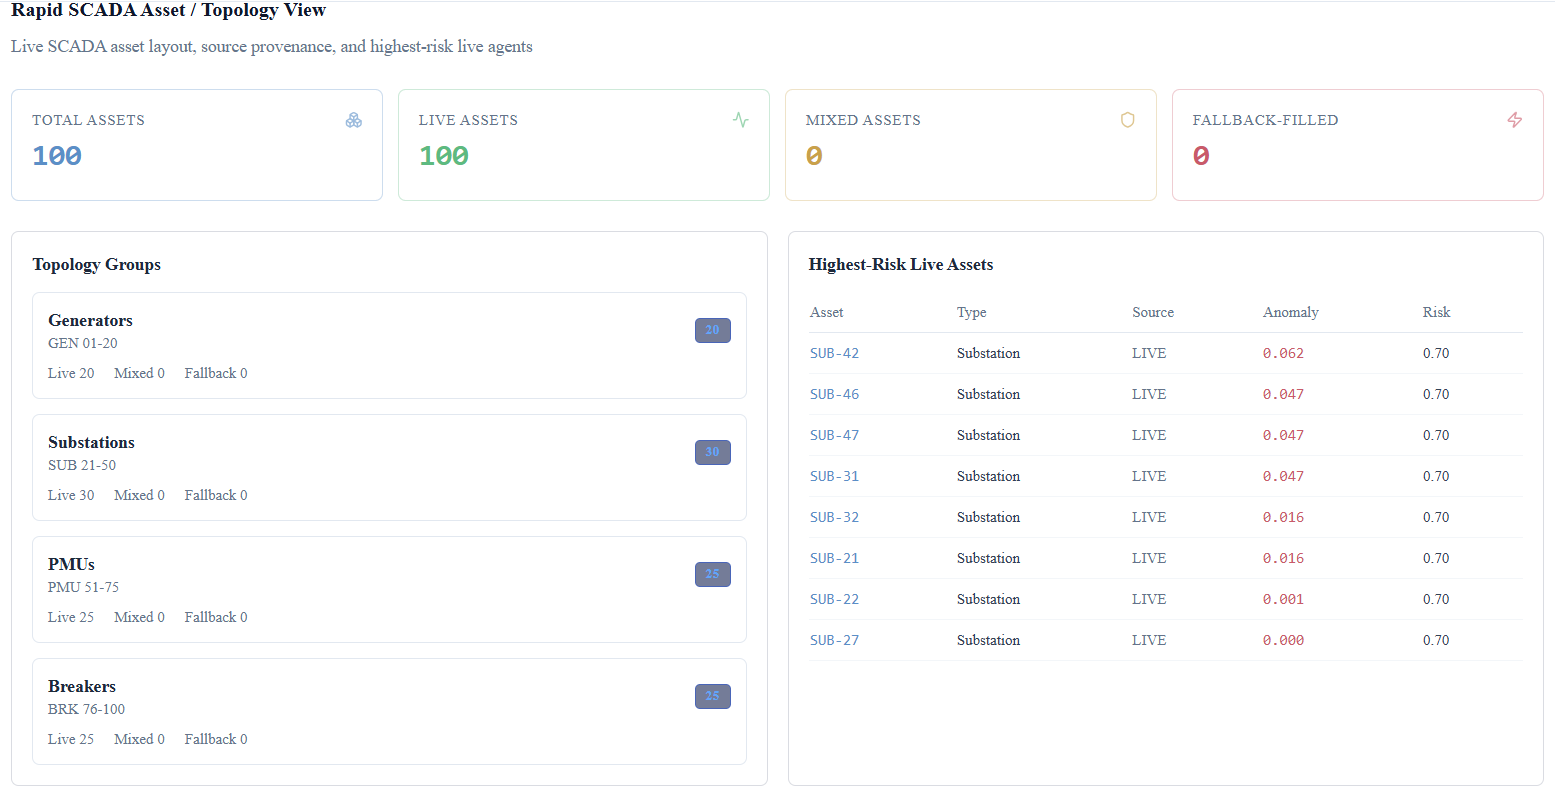
\includegraphics[width=0.95\textwidth]{FigRapid_SCADA_Asset_Topology_View.png}}
\caption{Rapid SCADA asset topology view showing the 100-agent grid layout across four asset classes.}
\label{fig:scada_topology}
\end{figure}

% ------------------------------------------------------------
\subsection{Tier 2: Feature Processing and Baseline Mapping}
% ------------------------------------------------------------

The feature processing tier transforms raw telemetry into normalised deviation vectors that quantify how far each observation departs from its expected baseline. The feature space is divided into two complementary domains.

\par \vspace{0.35cm}
\textbf{Physical Features.} Physical features capture the electrical and operational state of each agent and include measurements such as voltage, current, frequency, power, and response time. These features reflect the behaviour of the underlying physical infrastructure and are the primary indicators of grid health.

\par \vspace{0.35cm}
\textbf{Cyber Features.} Cyber features capture the communication and network state of each agent and include measurements such as latency, packet loss, communication frequency, and data integrity. These features reflect the health of the supervisory communication network and serve as indicators of potential cyber intrusions or network degradation.

\par \vspace{0.35cm}
\textbf{Baseline Specification.} Baselines are type-specific and hand-engineered for each asset class. Each feature within each asset type has a defined nominal baseline value and an associated threshold that represents the acceptable range of deviation. The baselines encode domain knowledge about normal operating conditions for generators, substations, PMUs, and breakers respectively. Table~\ref{tab:gen_baseline} illustrates the baseline profile for the generator (GEN) asset class as a representative example.

\begin{table}[H]
\centering
\caption{Generator (GEN) baseline profile: nominal values and thresholds.}
\label{tab:gen_baseline}
\begin{tabular}{llcc}
\hline
\textbf{Domain} & \textbf{Feature} & \textbf{Baseline ($b$)} & \textbf{Threshold ($\tau$)} \\
\hline
Physical & Voltage     & 230.0 V   & 10.0 V  \\
Physical & Frequency   & 50.0 Hz   & 1.0 Hz  \\
Physical & Current     & 100.0 A   & 20.0 A  \\
Physical & Power       & 23.0 kW   & 5.0 kW  \\
Physical & Response Time & 3.3 ms  & 5.0 ms  \\
\hline
Cyber    & Latency       & 0.17 (ratio) & 0.5  \\
Cyber    & Packet Loss   & 0.004       & 0.05 \\
Cyber    & Integrity     & 0.99        & 0.2  \\
Cyber    & Comm Frequency & 0.79       & 0.5  \\
\hline
\end{tabular}
\end{table}

\par \vspace{0.35cm}
\textbf{All Asset-Class Baseline Profiles.} Table~\ref{tab:gen_baseline} showed the GEN profile. The remaining three asset classes each carry distinct calibrated baselines that reflect their different operational roles within the grid. Table~\ref{tab:all_baselines} presents the complete per-type nominal baseline values for the key physical and cyber features across all four classes.

\begin{table}[H]
\centering
\caption{Per-type baseline profiles for all four agent classes: nominal values for primary features.}
\label{tab:all_baselines}
\renewcommand{\arraystretch}{1.25}
\begin{tabular}{|l|c|c|c|c|c|c|}
\hline
\textbf{Agent Class} & \textbf{Voltage (V)} & \textbf{Current (A)} & \textbf{Latency} & \textbf{Pkt Loss} & \textbf{Integrity} & \textbf{Comm Freq} \\
\hline
GEN & 231.0 & 13.0 & 0.17 & 0.003 & 0.99 & 0.80 \\
\hline
SUB & 189.0 (load) & 4.0 & 0.15 & 0.003 & 0.98 & 0.78 \\
\hline
PMU & 231.0 & 100.0 & 0.12 & 0.003 & 0.99 & 0.81 \\
\hline
BRK & 1.0 (status) & 0.0 & 0.17 & 0.004 & 0.99 & 0.80 \\
\hline
\end{tabular}
\end{table}

\par \vspace{0.25cm}
\noindent
The profiles encode the different physical roles of each class. Substations report a lower voltage (189~V as load-side) and a much lower current (4~A) compared with generators. PMUs report very high current (100~A) because they measure line current at the transmission level, and they have a lower latency baseline (0.12) reflecting their high-frequency synchronised measurement rate. Breakers report a voltage of 1.0 mapped to status (1 = closed, 0 = open) and zero current because they are switching devices rather than energy carriers. Using separate per-type baselines rather than a single fleet-wide average prevents the deviation scorer from systematically flagging breakers for having near-zero current, or PMUs for having high current, which is the normal condition for each class.

\par \vspace{0.35cm}
\textbf{Normalisation.} Each observed feature value is normalised against its baseline using the following transformation:
\begin{equation}
z_{j} = \frac{x_{j} - b_{j}}{\tau_{j}}
\label{eq:normalisation}
\end{equation}
where $x_{j}$ is the observed value of feature $j$, $b_{j}$ is the baseline value, and $\tau_{j}$ is the threshold. The resulting normalised value $z_{j}$ expresses the observation as a multiple of its acceptable deviation, which allows direct comparison across different feature types and asset classes.

% ------------------------------------------------------------
\subsection{Tier 3: Multi-Layer Anomaly Detection and Audit Intelligence}
% ------------------------------------------------------------

Tier~3 is the core analytical engine of the framework. It comprises multiple detection layers that operate in concert to identify anomalies, classify attack types, produce risk scores, determine audit actions, and generate human-readable explanations. The following subsections describe each component in detail.

\par \vspace{0.35cm}
\textbf{Statistical Deviation Scoring.}

\par \vspace{0.2cm}
The statistical deviation scorer computes a weighted composite score for each agent at each timestep by measuring the root-mean-square deviation of physical and cyber features from their respective baselines~\cite{priyadarsini2025}. For agent $i$ at time $t$, the deviation score is computed as:
\begin{equation}
S_{i}(t) = w_{i} \left( d_{x} + d_{y} \right)
\label{eq:deviation_score}
\end{equation}
where $d_{x}$ and $d_{y}$ denote the physical and cyber deviation components respectively. The physical deviation is defined as:
\begin{equation}
d_{x} = \sqrt{ \frac{1}{n_{x}} \sum_{j=1}^{n_{x}} \left( \frac{x_{j} - b_{x,j}}{\tau_{x,j}} \right)^{2} }
\label{eq:physical_deviation}
\end{equation}
where $n_{x}$ is the number of physical features, $x_{j}$ is the observed value, $b_{x,j}$ is the physical baseline, and $\tau_{x,j}$ is the physical threshold. The cyber deviation $d_{y}$ is computed analogously over the cyber feature set. The weight $w_{i}$ captures the relative importance of agent $i$ in the grid topology and can be adjusted to reflect criticality.

\par \vspace{0.35cm}
\textbf{LSTM Temporal Detector.}

\par \vspace{0.2cm}
The LSTM-based temporal detector is designed to capture sequential dependencies in agent behaviour that may not be apparent from instantaneous deviation scores alone. The detector employs a dual-branch architecture comprising a physical grid branch and a network/cyber branch. Each branch processes a sliding window of the most recent timesteps, producing a representation of the agent's recent temporal trajectory. In the experiment workspace, each branch receives 3 physical and 4 cyber features (7 total) as defined by the simulation environment; in the SCADA live workspace, each branch receives 5 physical and 4 cyber features (9 total) as provided by the SCADA adapter's type-specific feature mapping.

\par \vspace{0.2cm}
The two branch outputs are fused in a first-stage operation using fixed weights ($w_{\text{grid}} = 0.58$, $w_{\text{network}} = 0.42$) to produce a single calibrated anomaly probability $p_{\text{fused}}$. The grid branch carries the higher weight because physical instability is the primary threat surface in the power grid context. Temperature scaling is applied to the raw output logits before the sigmoid activation to ensure that the resulting probability is well-calibrated. This Stage~1 fusion happens entirely within the LSTM module, before the output is passed on to the ensemble layer.

\par \vspace{0.35cm}
\textbf{Stage~2 Weighted Ensemble Fusion.}

\par \vspace{0.2cm}
It is important to distinguish this second-stage fusion from the Stage~1 dual-branch fusion described above. Stage~1 fuses the two LSTM branches (physical vs.\ cyber) to produce a single probability. Stage~2 fuses two entirely different evidence sources, the statistical deviation scorer and the LSTM-based temporal detector, to produce a hybrid confidence estimate. The Stage~2 ensemble combines $p_{\text{fused}}$ from Stage~1 with the deviation-derived confidence to form the final decision signal. The deviation score and the fused LSTM probability are combined through a weighted ensemble to produce a hybrid confidence value for each agent at each timestep:
\begin{equation}
\text{hybrid\_conf}_{i}(t) = w_{\text{dev}} \cdot \text{dev\_conf}_{i}(t) + w_{\text{prob}} \cdot \text{prob\_support}_{i}(t) + \text{suspicion\_credit}_{i}(t)
\label{eq:hybrid_conf}
\end{equation}
where $w_{\text{dev}} = 0.48$ and $w_{\text{prob}} = 0.52$ are the ensemble weights for the deviation-based confidence and the LSTM probability support respectively. The suspicion credit term accumulates evidence over time for agents that exhibit borderline behaviour: each timestep in which an agent's LSTM probability exceeds a soft threshold adds a small increment to the credit, while consecutive normal readings decay the credit back toward zero. This way, agents with repeated borderline readings get escalated over time, even when no single observation on its own is decisive. The binary anomaly flag is triggered only when multiple conditions from both the deviation and probability branches agree:
\begin{equation}
a_{i}(t) =
\begin{cases}
1 & \text{if deviation AND probability conditions are satisfied} \\
0 & \text{otherwise}
\end{cases}
\label{eq:anomaly_flag}
\end{equation}

Requiring both detectors to agree prevents isolated spikes in either the statistical or temporal detector from triggering false positives.

\par \vspace{0.35cm}
\textbf{Multi-Layer Multi-Detector Architecture.}

\par \vspace{0.2cm}
Beyond the ensemble fusion, the system implements a multi-layer detection architecture that provides specialised detection capabilities for different attack and fault types. Each layer operates independently and contributes to the final anomaly determination through an OR-with-precedence combiner. Figure~\ref{fig:layerc_arch_ch3} shows the full layout including the four Layer C sub-detectors.

\begin{figure}[H]
\centering
\fbox{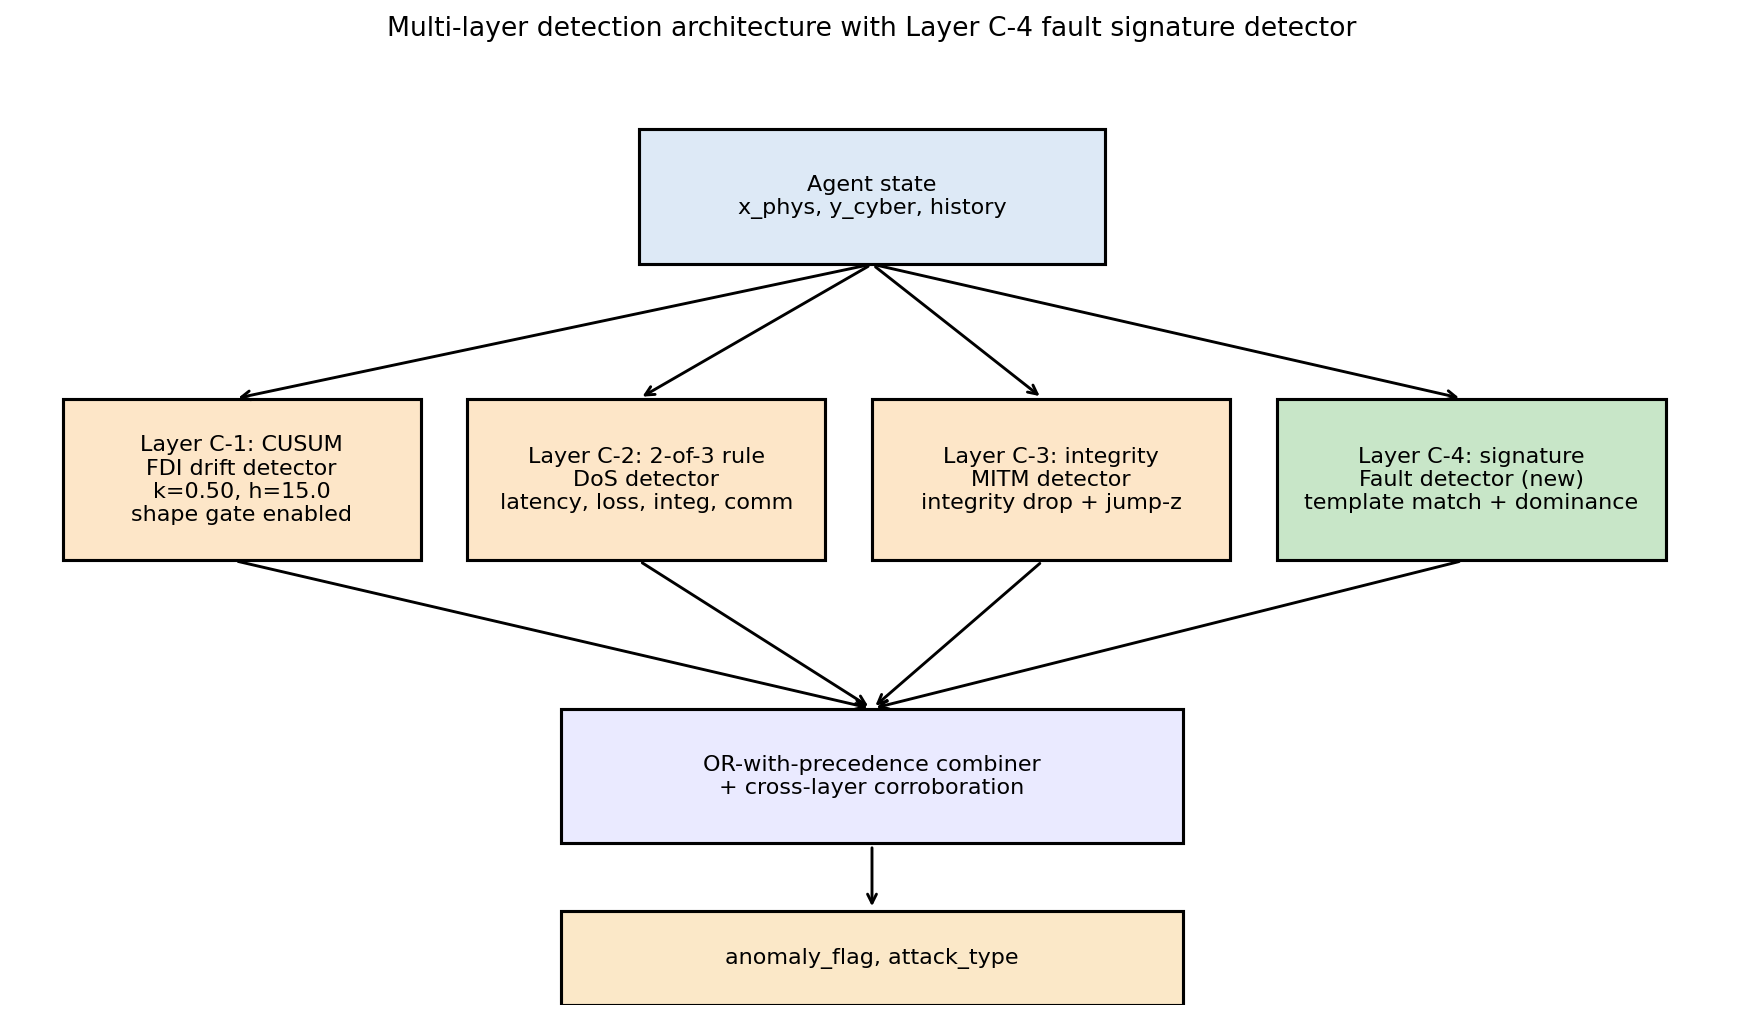
\includegraphics[width=0.95\textwidth]{Fig_LayerC_Architecture.png}}
\caption{Multi-layer detection architecture. The agent state feeds the four Layer C sub-detectors (CUSUM for FDI, 2-of-3 for DoS, integrity jump for MITM, and signature template for faults). Their outputs are merged by an OR-with-precedence combiner with cross-layer corroboration.}
\label{fig:layerc_arch_ch3}
\end{figure}

\par \vspace{0.2cm}
\textit{Layer A, Calibrated LSTM Threshold.} Layer~A applies a strict threshold on the calibrated LSTM output. An agent is flagged by this layer when its predicted anomaly probability satisfies $p \geq 0.80$ and its deviation score satisfies $S \geq 3.60$. This layer captures high-confidence anomalies where both the temporal model and the statistical scorer independently indicate strong evidence of deviation.

\par \vspace{0.2cm}
\textit{Layer B, Temporal Accumulator.} Layer~B implements a sustained suspicion detector that flags agents exhibiting moderate but persistent anomalous behaviour. An agent is flagged by this layer when its LSTM anomaly probability exceeds $p \geq 0.55$ for at least 5 consecutive timesteps within a rolling window of 6 timesteps. This layer is designed to detect slow-onset or gradually escalating anomalies that may not trigger the high-confidence threshold of Layer~A at any individual timestep but collectively represent a sustained departure from normal behaviour. Layer~B is operational in the current implementation, but an earlier design explored a second suppression tier (Tier-B) sitting between Layer~A and Layer~C to apply additional corroboration filtering. Multiple variants of Tier-B were evaluated, criticality-weighted gating, anomaly-spike-based gating, and percentile-based filtering, and all variants were found to reduce the false positive rate only marginally while producing a measurable drop in recall. The operating point of 94.23\% per-step accuracy with 100\% aggregate recall was judged to be more defensible than any Tier-B configuration tested, so Tier-B was removed and the architecture settled on the current three-layer layout (Layer~A, Layer~B, Layer~C).

\par \vspace{0.2cm}
\textit{Layer C: Attack and Fault Specific Detectors.} Layer~C comprises four specialised sub-detectors, each targeting a specific class of cyber-physical attack or physical fault:

\begin{itemize}
    \item \textbf{Layer C-1: CUSUM Drift Detector with Shape Gate (FDI).} This detector implements a two-sided cumulative sum on the physical residuals. The algorithm uses sensitivity $k = 0.50$ and alarm threshold $h = 15.0$ over a sliding window of 8 consecutive timesteps. Beyond the cumulative test, a shape gate is applied at the most recent step: at least two of the three FDI signature directions ($z[0] > 0.5$, $z[1] > 0.5$, $z[2] < -0.5$) must agree before the layer fires. This filter removes cumulative drifts that come from random noise rather than a coherent FDI signature, while keeping the layer responsive to real injections whose residual already matches the multi feature pattern~\cite{liu2009false}\cite{yan2020false}.

    \item \textbf{Layer C-2: Network Rule Detector for Denial of Service (DoS).} A weighted score is computed across all four cyber features (latency ratio, packet loss, integrity drop, and communication drop), with weights $0.20, 0.30, 0.30, 0.20$ respectively. The layer fires when the weighted score exceeds $0.45$, with a guard that suppresses the fire when integrity dominates and latency or packet loss are both weak (in that case the event is left to Layer C-3). This rule based formulation reduces false positives arising from transient network congestion.

    \item \textbf{Layer C-3: Integrity and Temporal Jump Detector for MITM.} The layer combines two signals~\cite{sadeghi2015security}: an integrity drop of at least $35\%$ from baseline, and a baseline aware jump z score of at least $2.5\sigma$. A guard vetoes the fire when latency and packet loss are both elevated (a DoS pattern). Both signals are required, which keeps precision high against legitimate operational transients.

    \item \textbf{Layer C-4: Signature Template Detector for Physical Faults (new contribution).} The layer template matches the physical residual against the three documented fault signatures (voltage sag, overcurrent, frequency deviation). It uses a primary z floor of $2.2$, a dominance ratio of $2.0$ between the primary feature and the strongest other feature, and a cyber guard of $2.5$ that vetoes the fire whenever any cyber channel deviates strongly (which would indicate a cyber attack rather than a physical fault). The detector fills a gap in the earlier architecture, where physical faults relied on fallback signature matching from the deviation pipeline and were frequently mistyped as FDI; with C-4 in place, the FAULT class is now identified with the same per type confidence as the cyber attack classes.
\end{itemize}

\par \vspace{0.2cm}
\textit{Combiner: OR-with-Precedence and Cross-Layer Corroboration.} The outputs of all layers are combined using an OR-with-precedence rule: if any layer fires, the agent is flagged as anomalous. When multiple layers fire simultaneously, the layer with the highest specificity (Layer~C, then Layer~A, then Layer~B) takes precedence for attack classification, and within Layer~C the new fault detector (C-4) takes precedence over CUSUM (C-1) when both fire on the same step, because the C-4 fire requires single feature dominance and quiet cyber channels, which is direct evidence against the FDI shape. A cross-layer corroboration gate is also applied after the per layer decisions: a flag raised purely by the deviation magnitude path (the severe deviation trigger) with low LSTM confidence ($p < 0.45$) and no Layer~C agreement is demoted to a clean prediction. This single rule removes the dominant noise driven false positive pattern without affecting any case where at least one detector signature is present.

\par \vspace{0.2cm}
\textit{Temporal Signature Classification.} Alongside the three-layer detectors, a lightweight temporal pattern classifier analyses the shape of the deviation trajectory over the most recent five timesteps to identify the physical signature of the anomaly. Four signature types are recognised:
\begin{itemize}
    \item \textbf{STEP}, an abrupt, sustained shift in one or more features (characteristic of FDI with a constant bias).
    \item \textbf{RAMP}, a linearly increasing deviation over time (characteristic of FDI with a drift component, or gradual load faults).
    \item \textbf{OSCILLATORY}, alternating positive and negative deviations with no persistent direction (characteristic of MITM measurement noise or sensor interference).
    \item \textbf{STABLE}, no significant change pattern detected (consistent with normal operation or a very slow developing fault).
\end{itemize}
The classified signature feeds into the five-class attack typing module described below, providing an additional discriminative signal beyond the instantaneous feature values.

\par \vspace{0.2cm}
\textit{Five-Class Attack Typing.} The system assigns each flagged agent one of five attack class labels using a weighted combination of the Layer~C detector outputs, the temporal signature, and the deviation magnitudes across physical and cyber domains:
\begin{itemize}
    \item \textbf{FDI (False Data Injection):} Physical features show a STEP or RAMP signature; CUSUM detector fires; cyber features are within normal range.
    \item \textbf{DOS (Denial of Service):} Network rule detector fires; latency, packet loss, and communication frequency conditions are triggered; physical features are largely unaffected.
    \item \textbf{MITM (Man-in-the-Middle):} Integrity-jump detector fires; OSCILLATORY signature present; both physical and cyber features show simultaneous noise.
    \item \textbf{FAULT (Physical Equipment Fault):} Physical features show large deviations consistent with hardware failure (voltage collapse, current spike); cyber features remain healthy; no network rule or MITM indicator present.
    \item \textbf{CHAIN (Coordinated Cross-Layer Attack):} Multiple Layer~C detectors fire simultaneously; both physical and cyber deviations are elevated; indicates a coordinated attack targeting multiple system layers at once.
\end{itemize}
The attack type label is reported alongside the anomaly flag in both the audit trail and the explainability output, so operators know not only that an anomaly was detected but also what class of event the system believes it is dealing with.

\par \vspace{0.2cm}
\textit{Tier-A False Positive Suppression.} To reduce spurious alerts, a suppression mechanism is applied at the output stage. An alert is suppressed only when all five of the following conditions are simultaneously satisfied: the score ratio falls below 3.50, the LSTM anomaly probability is below 0.60, the network intrusion probability is below 0.55, the hybrid confidence is below 1.05, and no behavioural signature from the Layer~C detectors is present. Requiring all five conditions to hold together ensures that only genuine low-evidence detections are suppressed. If any single condition is not met, for instance, the LSTM probability is elevated even when the score ratio is low, the alert is retained and passed through to the operator.

\begin{figure}[H]
\centering
\fbox{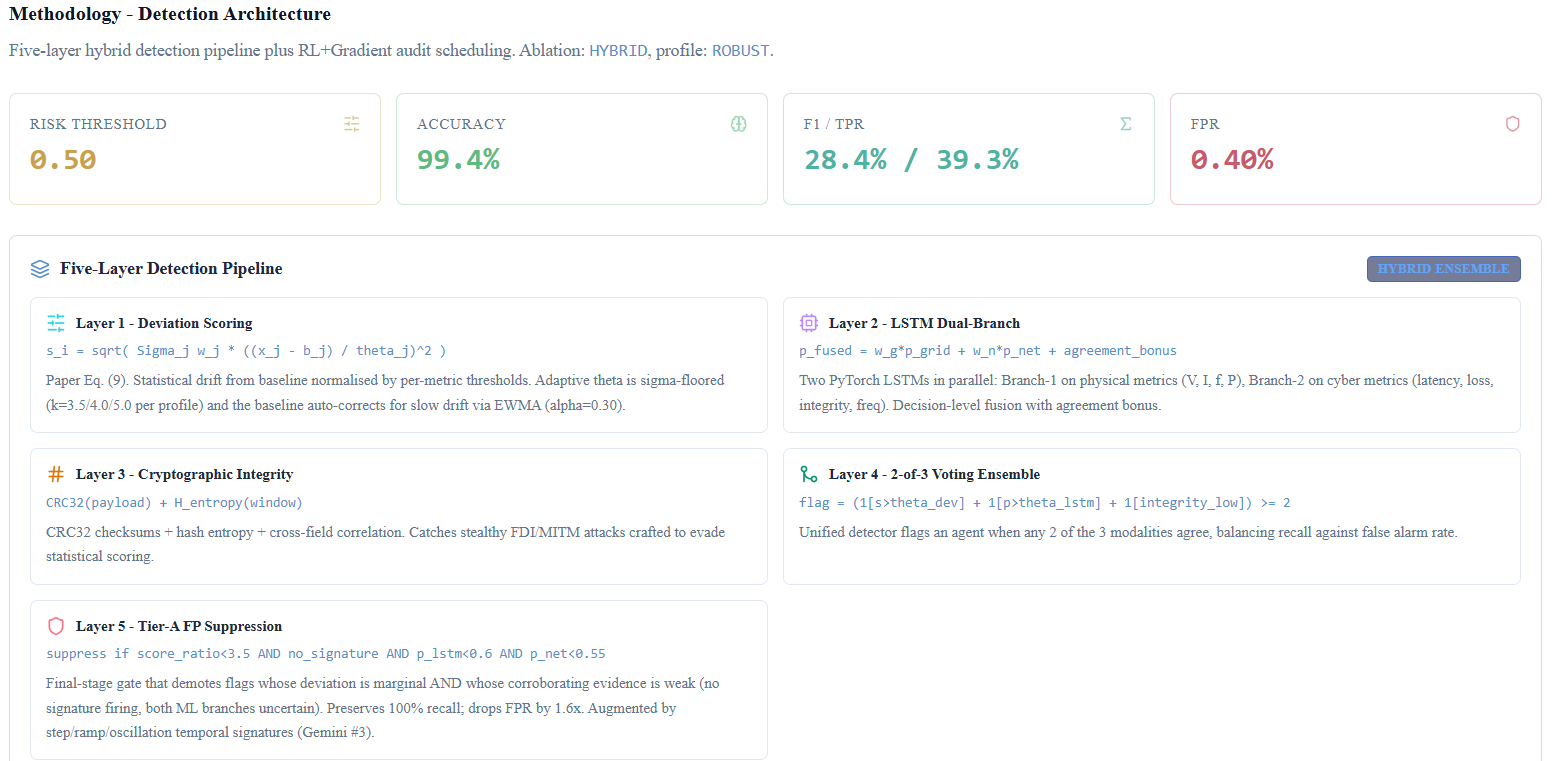
\includegraphics[width=0.95\textwidth]{FigMethodology_-_Detection_Architecture.png}}
\caption{Multi-layer detection architecture showing the three detection layers and the OR-with-precedence combiner.}
\label{fig:detection_architecture}
\end{figure}

\par \vspace{0.35cm}
\textbf{Audit Decision Logic.}

\par \vspace{0.2cm}
The audit decision module determines the appropriate audit frequency and escalation action for each agent based on the detection outputs and a hybrid optimisation strategy. The module combines reinforcement learning with gradient-based cost optimisation to balance detection effectiveness against audit cost.

\par \vspace{0.2cm}
\textit{Hybrid Scheduler.} The scheduler employs Q-learning~\cite{priyadarsini2025,ibrahim2023security} to adjust audit frequencies in response to observed anomaly patterns. The Q-learning agent maintains a state representation that encodes the current risk level and audit history of each grid agent, and selects actions that maximise a reward function balancing detection coverage and resource efficiency.

\par \vspace{0.2cm}
\textit{Cost Function.} The audit cost for agent $i$ operating at audit frequency $f_{i}$ is defined as:
\begin{equation}
C_{i} = C_{a} \cdot f_{i} + C_{f} \cdot \frac{R_{i}}{f_{i}}
\label{eq:cost_function}
\end{equation}
where $C_{a}$ is the per-audit cost, $C_{f}$ is the cost associated with undetected failures, and $R_{i}$ is the risk score of agent $i$. The first term penalises excessive auditing, while the second term penalises insufficient auditing of high-risk agents. The optimal audit frequency is obtained by differentiating the cost function with respect to $f_{i}$:
\begin{equation}
\frac{\partial C_{i}}{\partial f_{i}} = C_{a} - C_{f} \cdot \frac{R_{i}}{f_{i}^{2}}
\label{eq:cost_gradient}
\end{equation}

Setting this gradient to zero yields the analytically optimal frequency, which the gradient-based component uses to guide the Q-learning policy toward cost-efficient solutions.

\par \vspace{0.2cm}
\textit{Action Escalation.} Based on the combined risk assessment from the detection layers and the audit scheduler, the system assigns one of five escalation actions to each agent:

\begin{itemize}
    \item \textbf{NO\_ANOMALY:} The agent is operating within normal parameters. Standard monitoring continues at the baseline audit frequency.
    \item \textbf{LOG\_MONITOR:} A marginal deviation has been observed. The event is logged and the agent is placed under enhanced passive monitoring without changing the audit frequency.
    \item \textbf{INCREASE\_AUDIT:} Elevated risk has been detected. The audit frequency for the agent is increased to improve monitoring granularity.
    \item \textbf{ISOLATE\_NOTIFY:} A confirmed anomaly has been detected with high confidence. The agent is flagged for isolation and the operator is notified for manual review.
    \item \textbf{EMERGENCY\_SHUTDOWN:} A critical threat has been identified with sustained high-confidence evidence. The system recommends immediate shutdown of the affected agent and alerts the operator through the highest-priority notification channel.
\end{itemize}

Budget constraints are enforced throughout the scheduling process to ensure that the total audit cost across all agents does not exceed the allocated operational budget.

\par \vspace{0.35cm}
\textbf{Explainability.}

\par \vspace{0.2cm}
The explainability module generates per-agent, per-timestep explanations that identify the specific features contributing most to each anomaly detection. For each feature $j$, the contribution score is computed as:
\begin{equation}
c_{j} = \left( \frac{x_{j} - b_{j}}{\tau_{j}} \right)^{2}
\label{eq:feature_contribution}
\end{equation}
where $x_{j}$ is the observed value, $b_{j}$ is the baseline, and $\tau_{j}$ is the threshold. The relative importance of each feature is then computed as:
\begin{equation}
\text{relative}_{j} = \frac{c_{j}}{\sum_{k=1}^{n} c_{k}}
\label{eq:relative_importance}
\end{equation}

The top-$k$ physical features and top-$k$ cyber features are computed independently, so that the explanation always covers both domains. Each anomalous agent gets a set of reason codes describing the main drivers of the detection in plain terms, letting operators see not only that an anomaly was detected but also why it was flagged and which measurements are most concerning.

% ------------------------------------------------------------
\subsection{Tier 4: Visualisation and Operator Interface}
% ------------------------------------------------------------

The visualisation tier provides a web-based dashboard built with Next.js that serves as the primary operator interface. The dashboard is organised into the two workspaces described in Section~3.1, each offering a tailored set of views.

\par \vspace{0.35cm}
\textbf{Experiment Workspace.} The experiment workspace provides the following views for simulation-based evaluation and analysis:

\begin{itemize}
    \item \textbf{Risk Analytics:} Aggregated risk scores, distributions, and trends across the agent population.
    \item \textbf{Audit Trail:} A chronological record of all audit decisions, escalation actions, and detection events.
    \item \textbf{Response Workflow:} The current escalation state of each agent and the sequence of actions taken.
    \item \textbf{Timeline:} A temporal visualisation of anomaly events and audit actions across the simulation horizon.
    \item \textbf{Decision Explainability:} Per-agent feature-level explanations showing the top contributing features for each detection.
    \item \textbf{Asset Topology:} A graphical representation of the agent grid layout and inter-agent relationships.
    \item \textbf{Experiment Control:} Configuration and execution controls for launching, parameterising, and monitoring experiments.
    \item \textbf{Run History:} A record of all past experiment runs with their configurations and summary results.
\end{itemize}

\par \vspace{0.35cm}
\textbf{SCADA Live Workspace.} The SCADA live workspace provides the following views for real-time operational monitoring:

\begin{itemize}
    \item \textbf{Real-time Monitor:} Live telemetry readings for all 100 agents with colour-coded status indicators.
    \item \textbf{Threat Events:} A feed of detected anomalies and attack classifications with timestamps and severity levels.
    \item \textbf{Audit Trail:} A live chronological record of audit decisions and escalation actions applied to the operational grid.
    \item \textbf{SCADA Grid:} A grid view showing the current state of all agents with their deviation scores and anomaly flags.
    \item \textbf{Topology:} An interactive asset topology view reflecting the live status of generators, substations, PMUs, and breakers.
    \item \textbf{Connectivity:} A connectivity status panel showing the health of the SCADA communication links and the bridge connection status.
\end{itemize}

\begin{figure}[H]
\centering
\fbox{
\includegraphics[width=0.95\textwidth]{FigExperiment_OperationOverview.png}}
\caption{Experiment workspace operations overview showing the primary dashboard views.}
\label{fig:experiment_overview}
\end{figure}

\begin{figure}[H]
\centering
\fbox{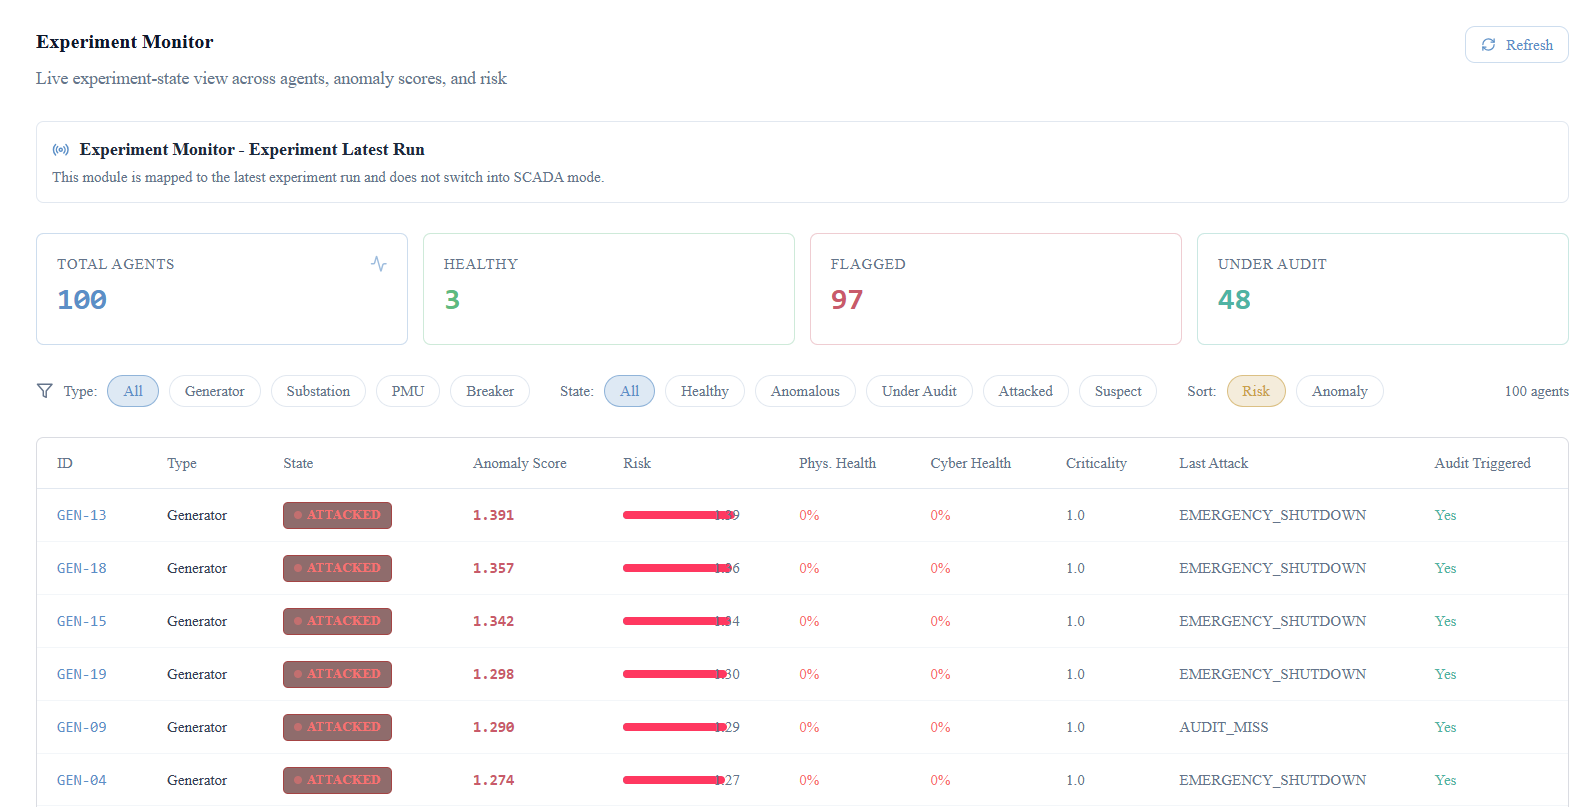
\includegraphics[width=0.95\textwidth]{FigExperiment_Monitor.png}}
\caption{Experiment workspace real-time monitor view displaying live telemetry readings and agent status indicators.}
\label{fig:experiment_monitor}
\end{figure}

\begin{figure}[H]
\centering
\fbox{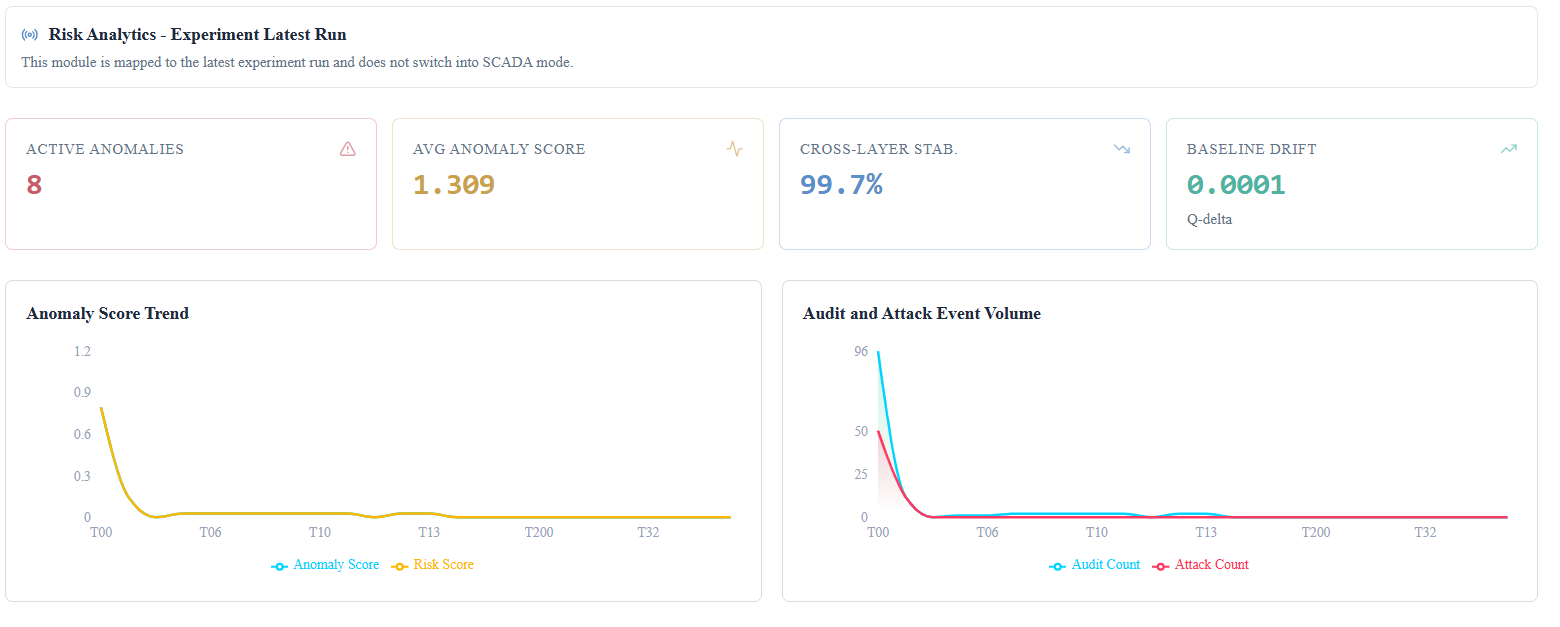
\includegraphics[width=0.95\textwidth]{FigExperiment_Risk_Analytics.png}}
\caption{Risk analytics view from the experiment workspace showing aggregated risk scores and distributions across the agent population.}
\label{fig:experiment_risk_analytics}
\end{figure}

\begin{figure}[H]
\centering
\fbox{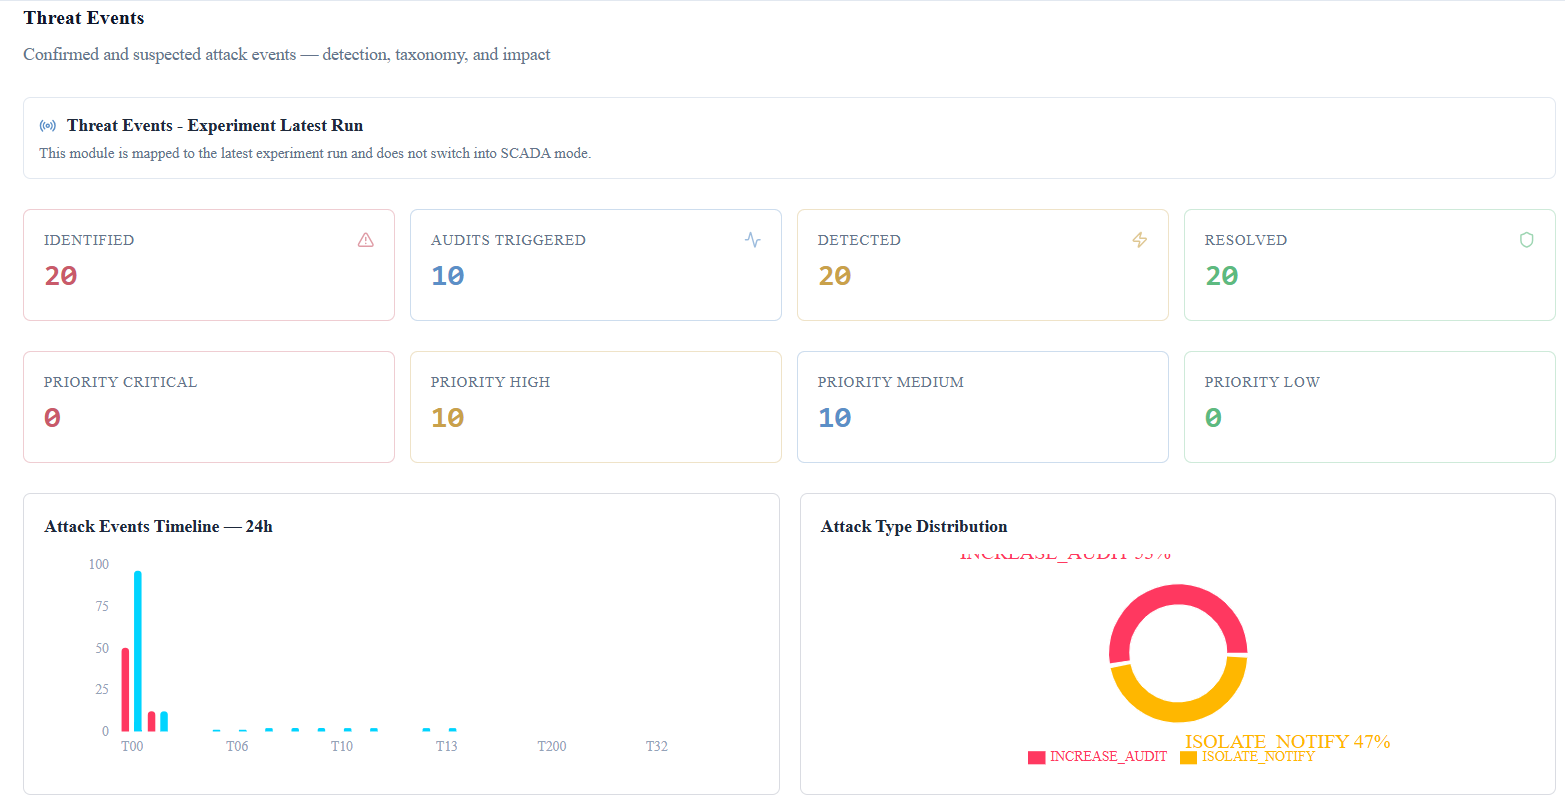
\includegraphics[width=0.95\textwidth]{FigExperiment_Threat_Events.png}}
\caption{Threat events feed from the experiment workspace showing detected anomalies and attack classifications with timestamps.}
\label{fig:experiment_threat_events}
\end{figure}

\begin{figure}[H]
\centering
\fbox{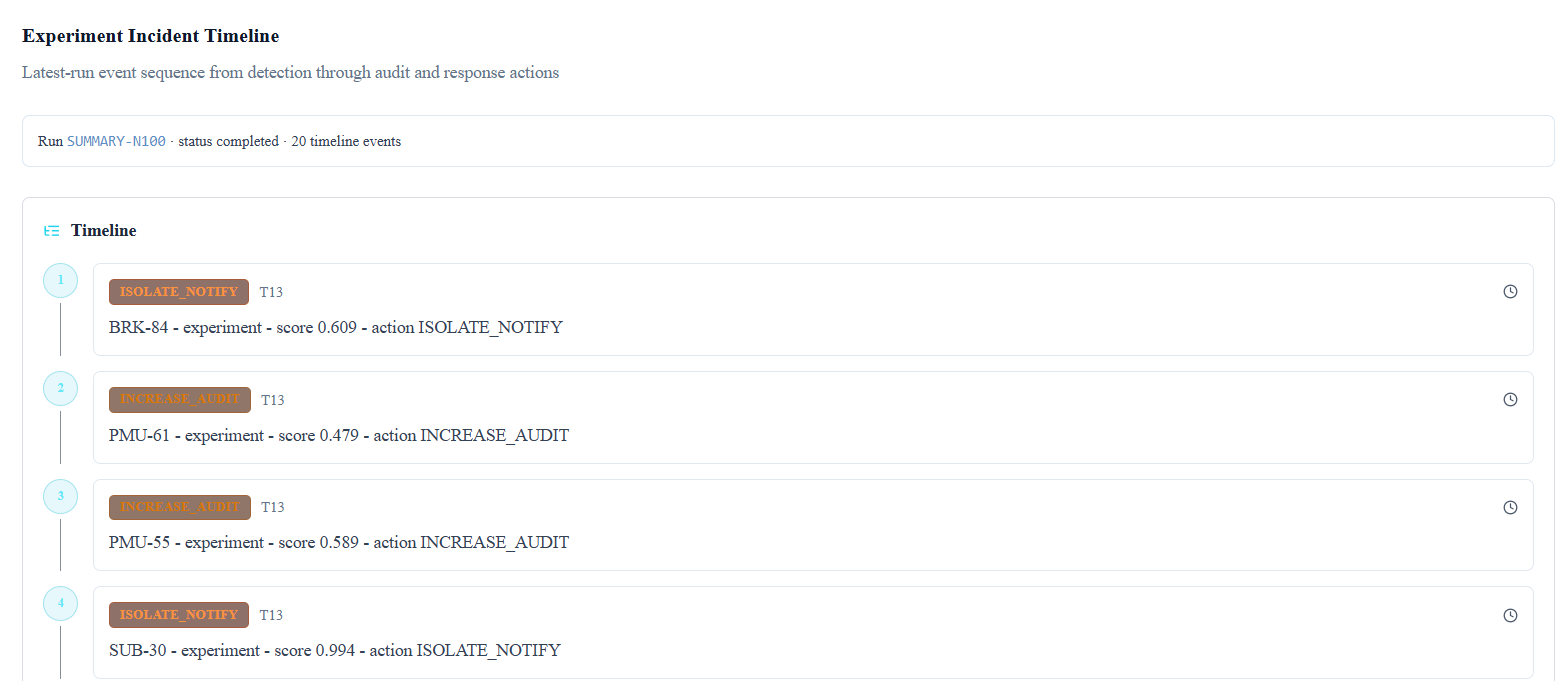
\includegraphics[width=0.95\textwidth]{FigExperiment_Timeline.png}}
\caption{Experiment workspace timeline view showing temporal distribution of anomaly events and audit actions across the simulation horizon.}
\label{fig:experiment_timeline}
\end{figure}

\begin{figure}[H]
\centering
\fbox{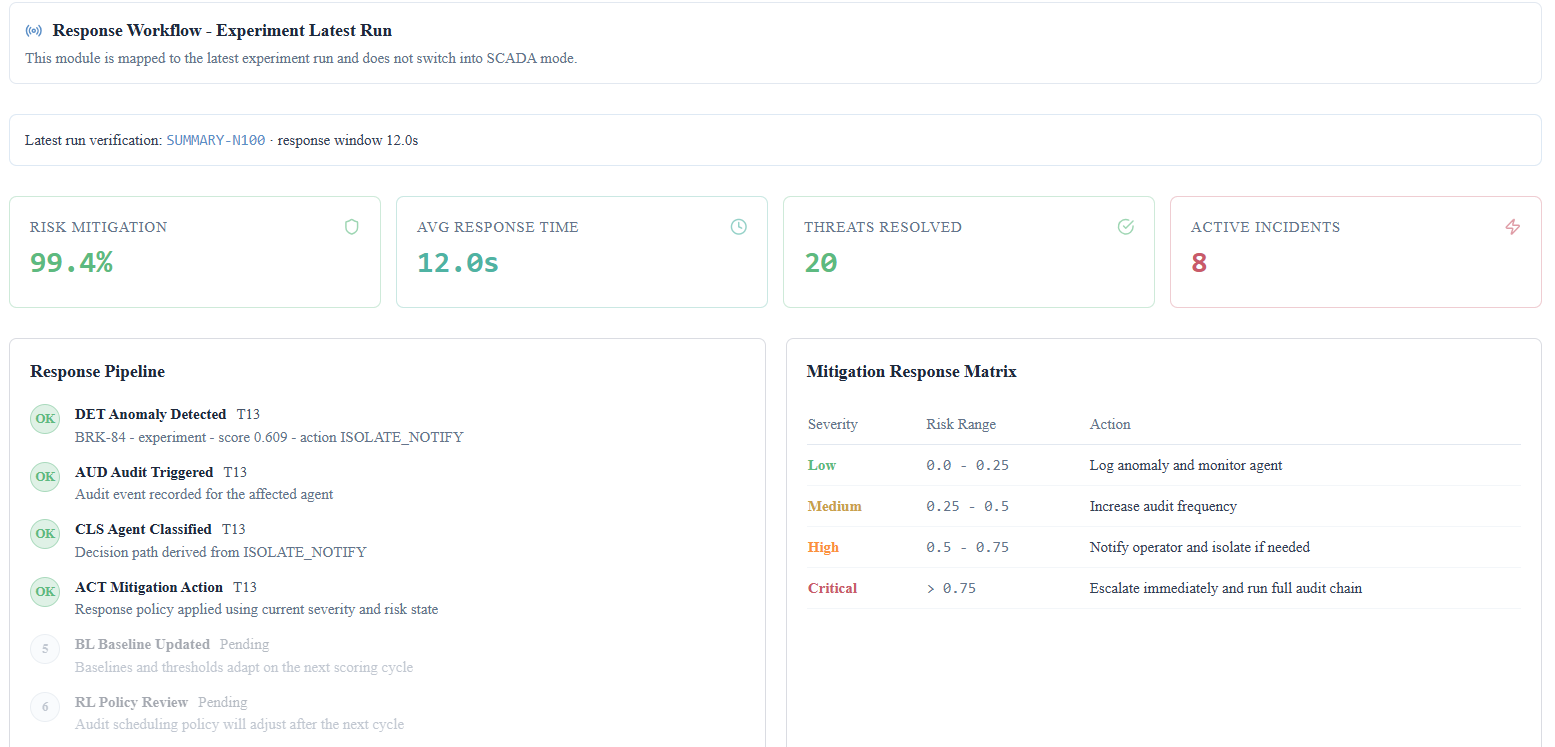
\includegraphics[width=0.95\textwidth]{FigExperiment_Response_Workflow.png}}
\caption{Response workflow view from the experiment workspace showing the current escalation state and sequence of actions for each agent.}
\label{fig:experiment_response_workflow}
\end{figure}

\begin{figure}[H]
\centering
\fbox{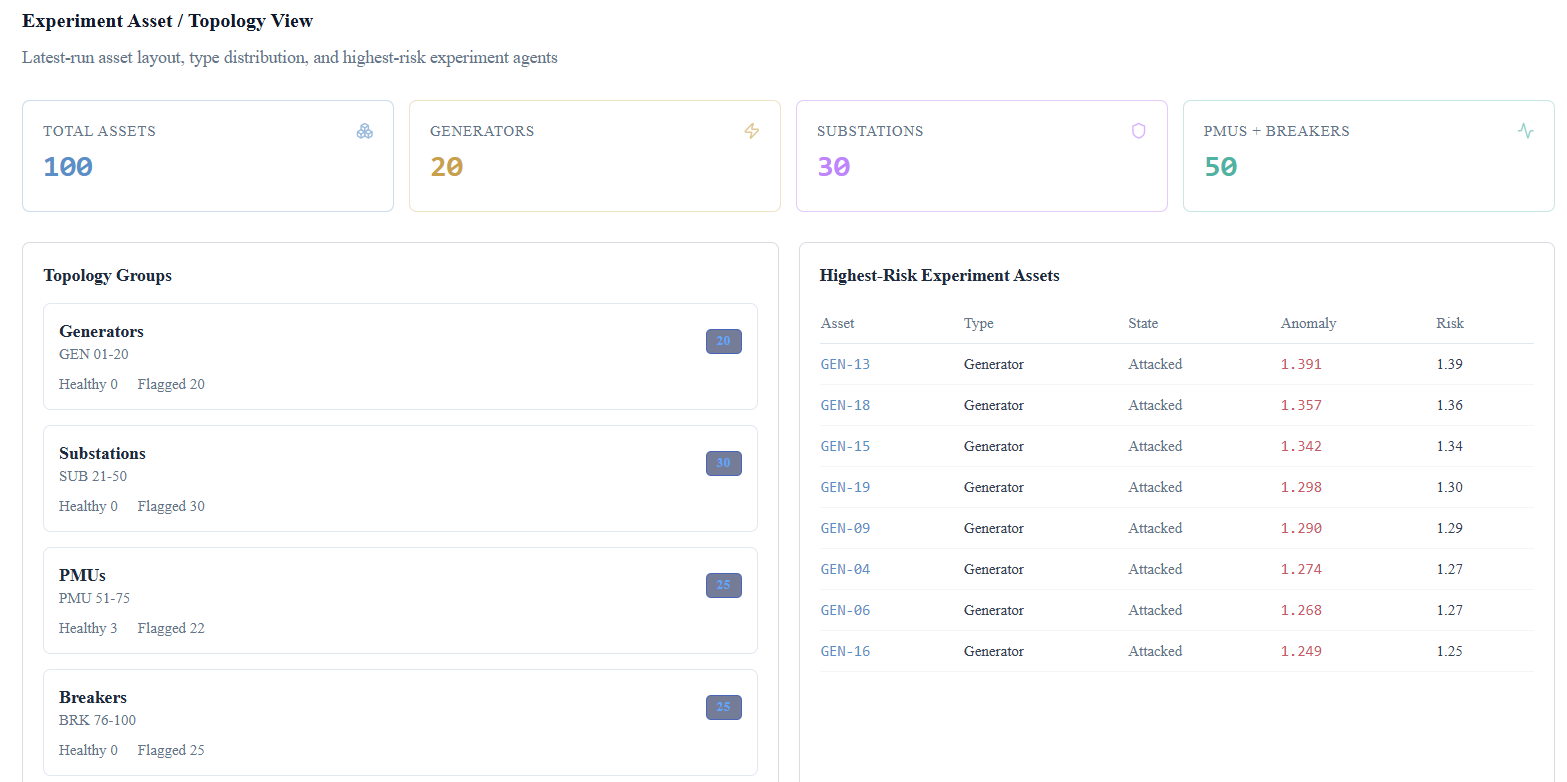
\includegraphics[width=0.95\textwidth]{FigExperiment_Asset_Topology_View.png}}
\caption{Asset topology view from the experiment workspace showing the graphical layout of agents and their inter-relationships.}
\label{fig:experiment_asset_topology}
\end{figure}

\begin{figure}[H]
\centering
\fbox{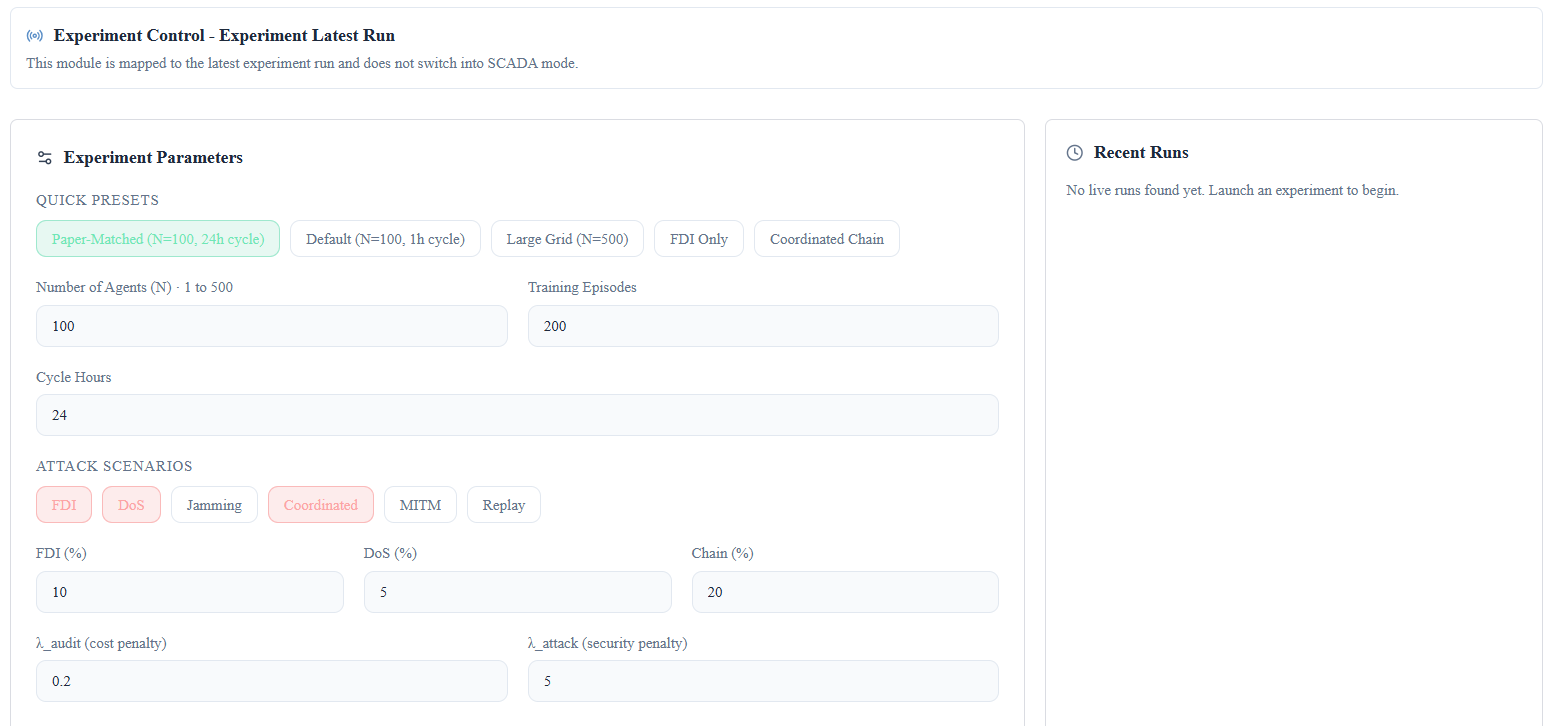
\includegraphics[width=0.95\textwidth]{FigExperiment_Control.png}}
\caption{Experiment control panel providing configuration and execution controls for launching, parameterising, and monitoring experiments.}
\label{fig:experiment_control}
\end{figure}

\par \vspace{0.35cm}
\noindent
Figures~\ref{fig:scada_ops_overview}--\ref{fig:scada_incident_timeline} present the dashboard views from the Rapid SCADA live workspace.

\begin{figure}[H]
\centering
\fbox{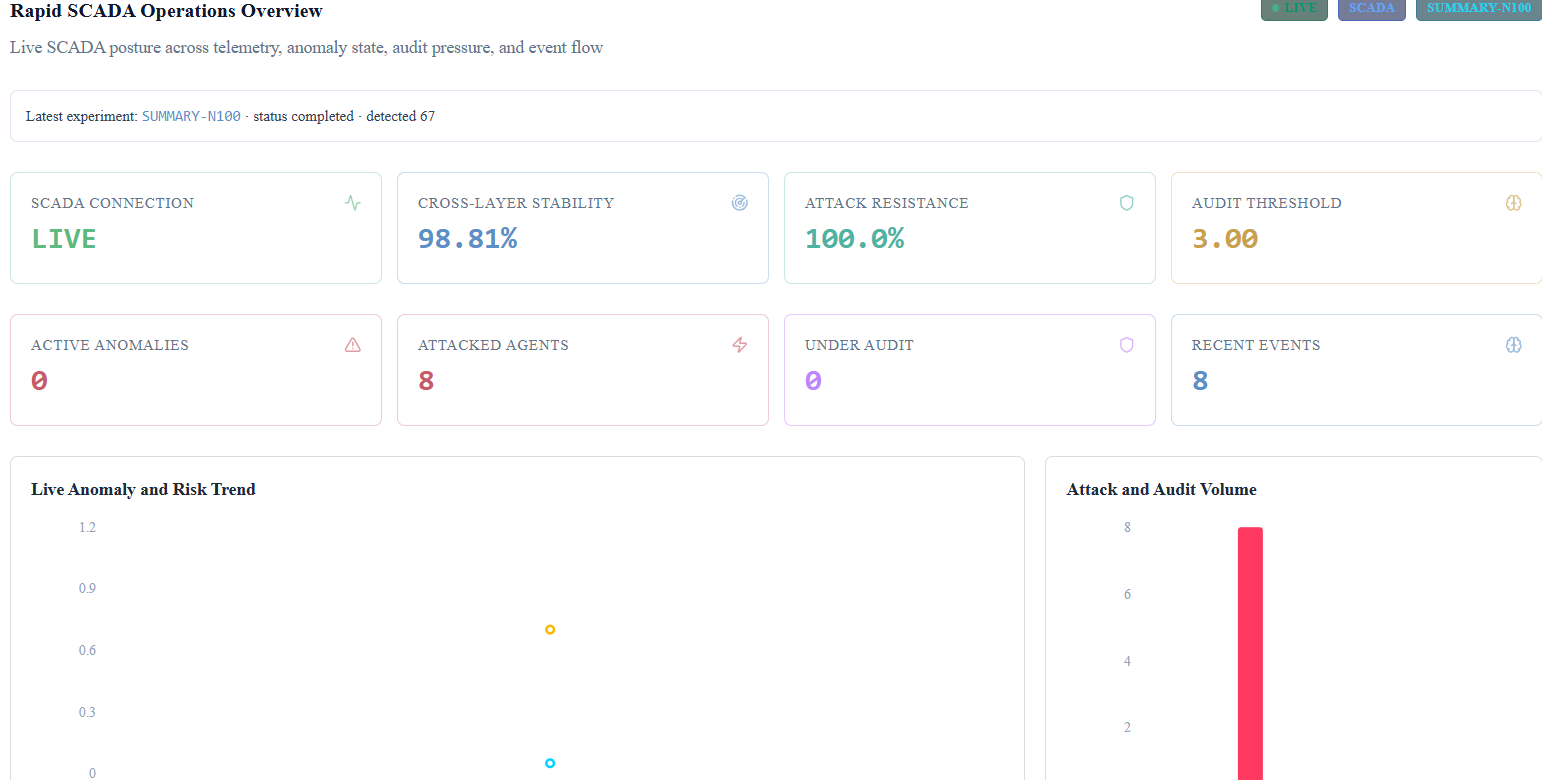
\includegraphics[width=0.95\textwidth]{FigRapid_SCADA_Operations_Overview.png}}
\caption{Rapid SCADA live workspace operations overview showing real-time monitoring status for the 100-agent grid.}
\label{fig:scada_ops_overview}
\end{figure}

\begin{figure}[H]
\centering
\fbox{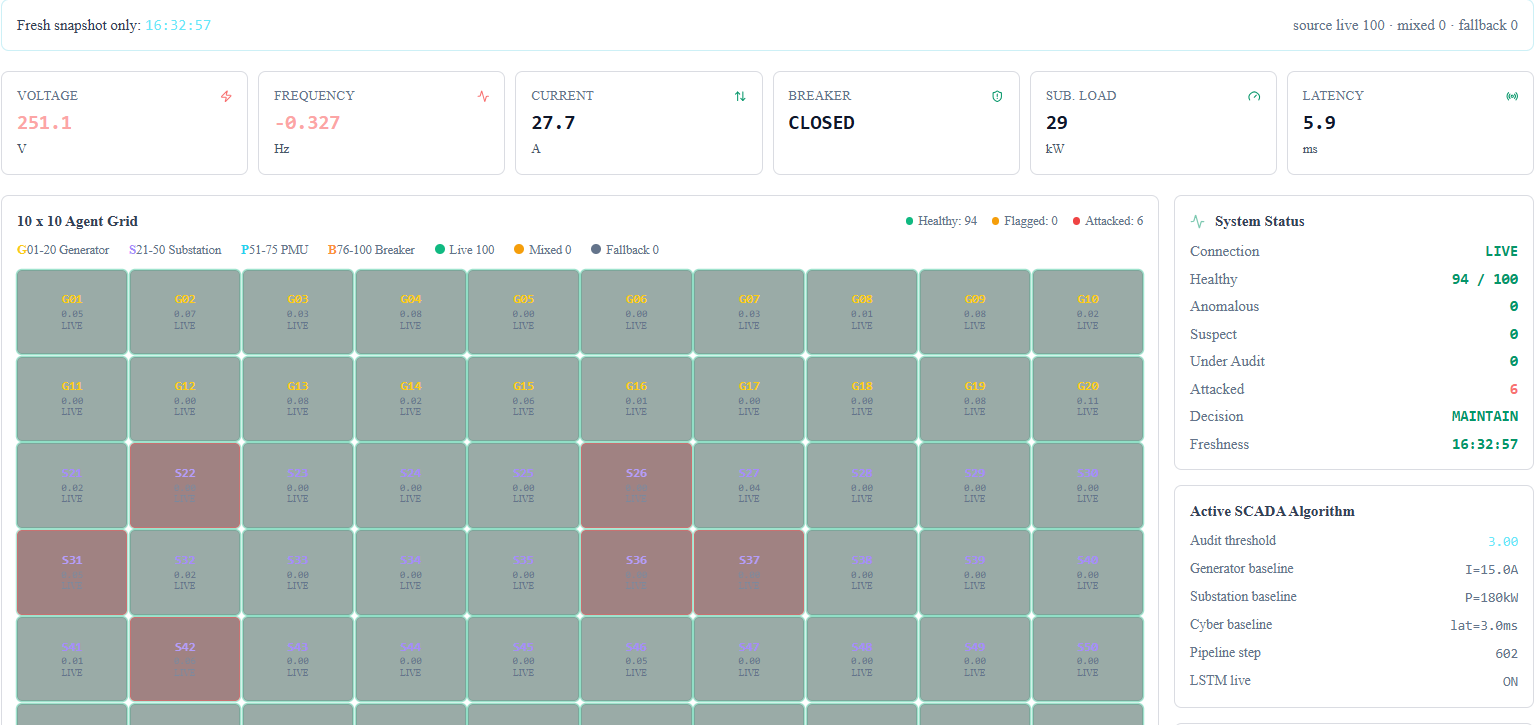
\includegraphics[width=0.95\textwidth]{FigGrid_With_The_Agents.png}}
\caption{SCADA grid view with 100 agents distributed across four asset classes.}
\label{fig:scada_grid_agents}
\end{figure}

\begin{figure}[H]
\centering
\fbox{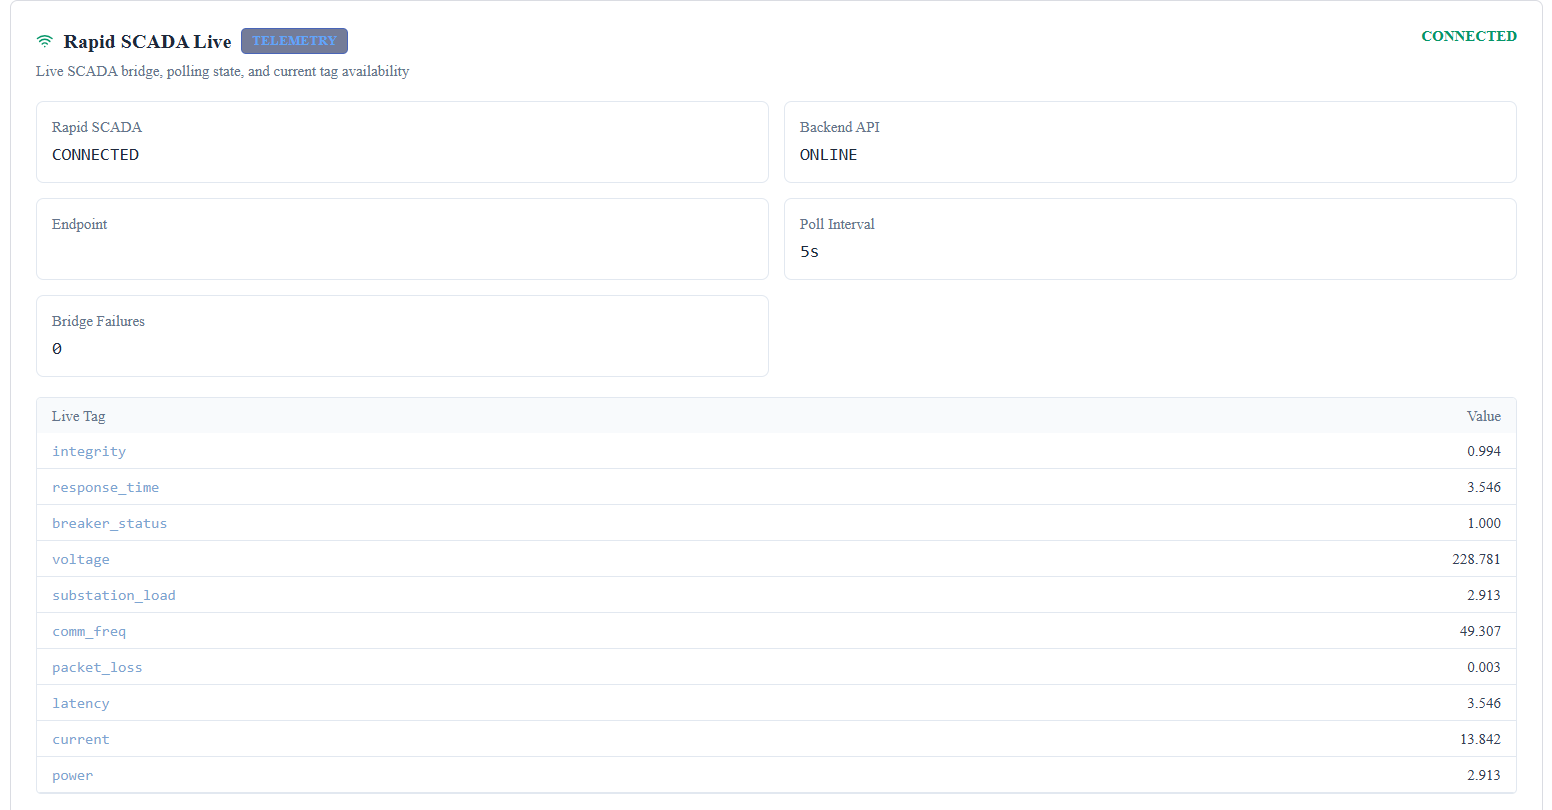
\includegraphics[width=0.95\textwidth]{FigRapid_SCADA_Connectivity.png}}
\caption{Connectivity status panel from the SCADA live workspace showing the health of communication links and bridge connection status.}
\label{fig:scada_connectivity}
\end{figure}

\begin{figure}[H]
\centering
\fbox{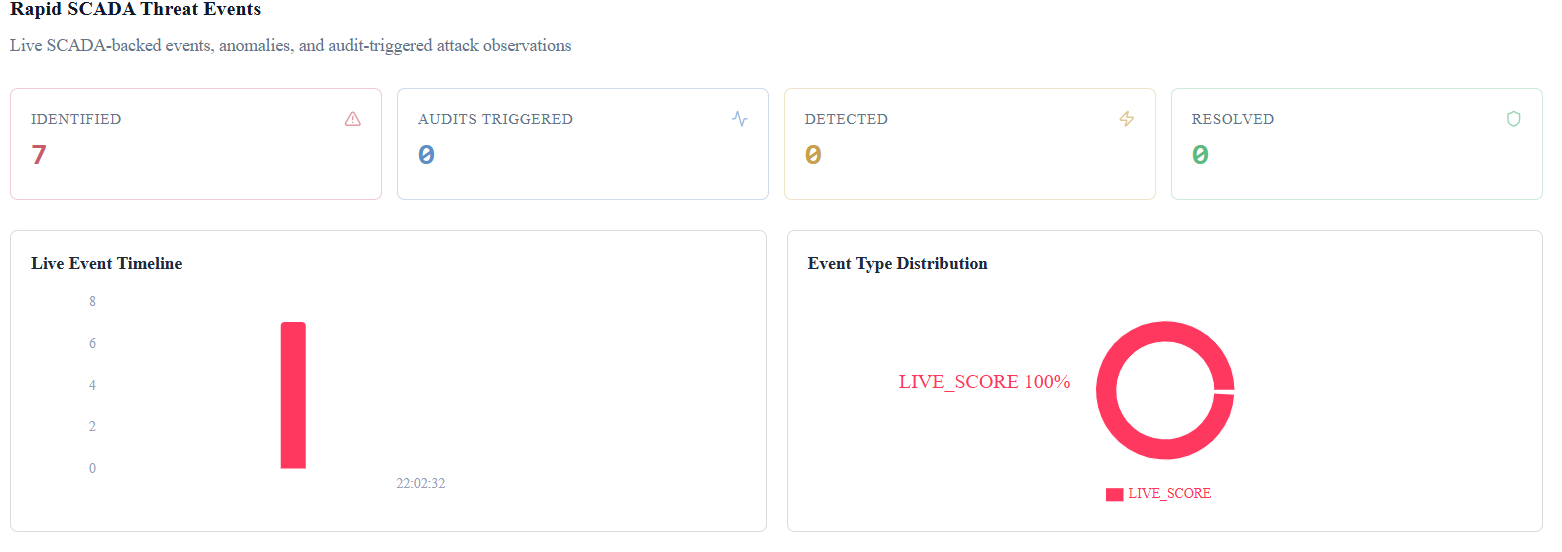
\includegraphics[width=0.95\textwidth]{FigRapid_SCADA_Threat_Events.png}}
\caption{Threat events feed from the SCADA live workspace displaying detected anomalies and their severity levels in real time.}
\label{fig:scada_threat_events}
\end{figure}

\begin{figure}[H]
\centering
\fbox{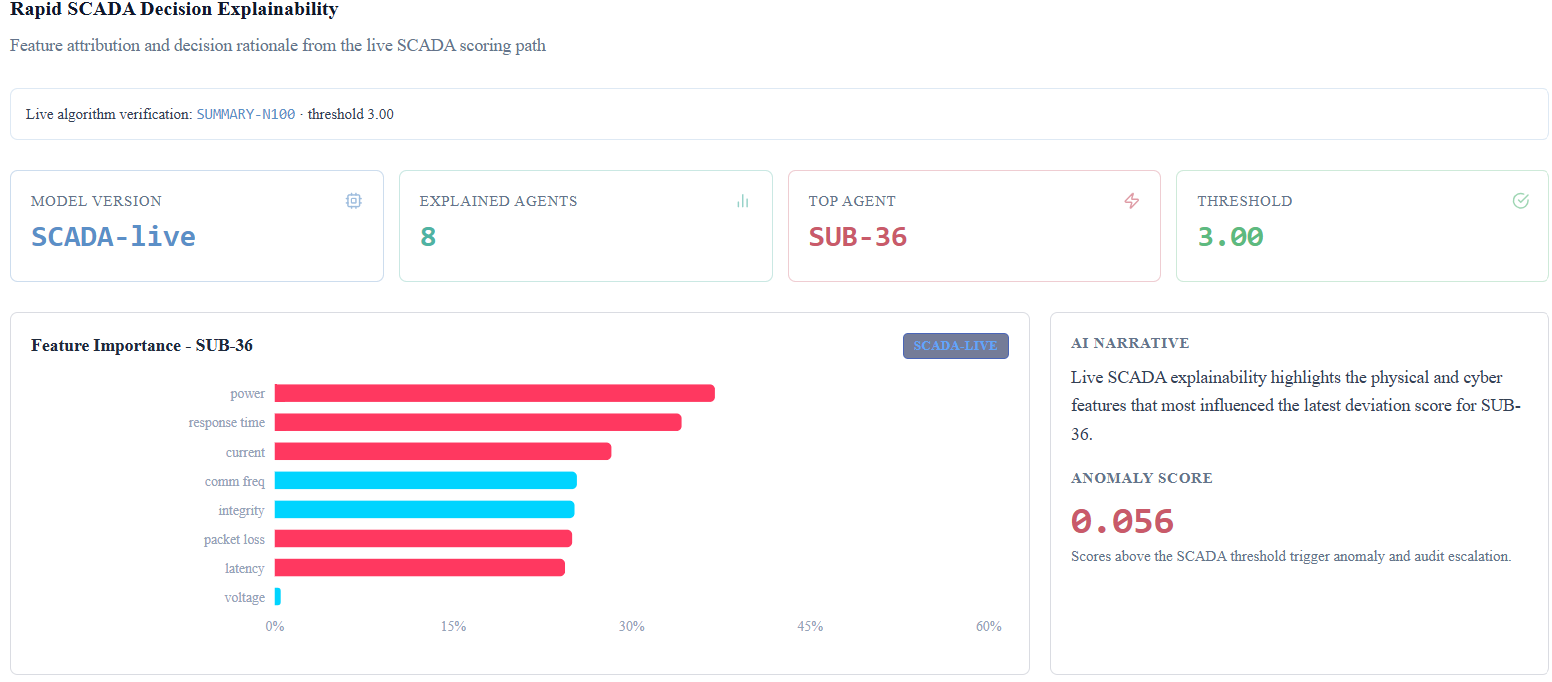
\includegraphics[width=0.95\textwidth]{FigRapid_SCADA_Decision_Explainability.png}}
\caption{Decision explainability view from the SCADA live workspace showing per-feature contribution rankings for a selected agent.}
\label{fig:scada_decision_xai}
\end{figure}

\begin{figure}[H]
\centering
\fbox{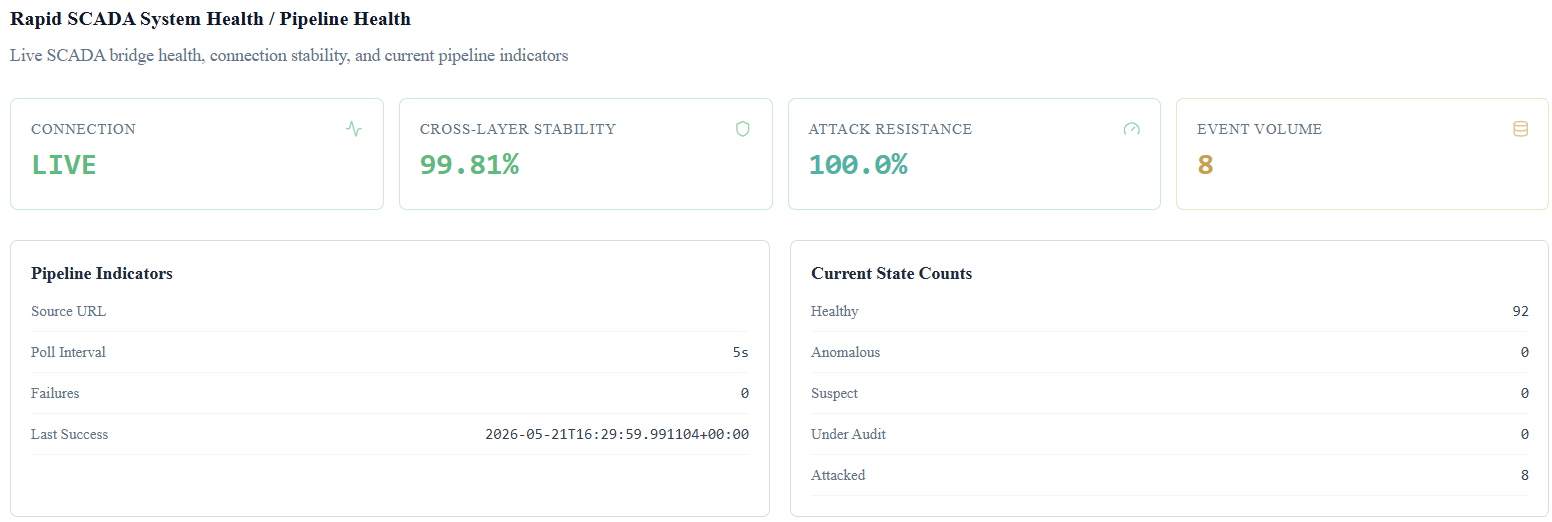
\includegraphics[width=0.95\textwidth]{FigRapid_SCADA_System_Health.png}}
\caption{System health view from the SCADA live workspace showing real-time status indicators for each subsystem component.}
\label{fig:scada_system_health}
\end{figure}

\begin{figure}[H]
\centering
\fbox{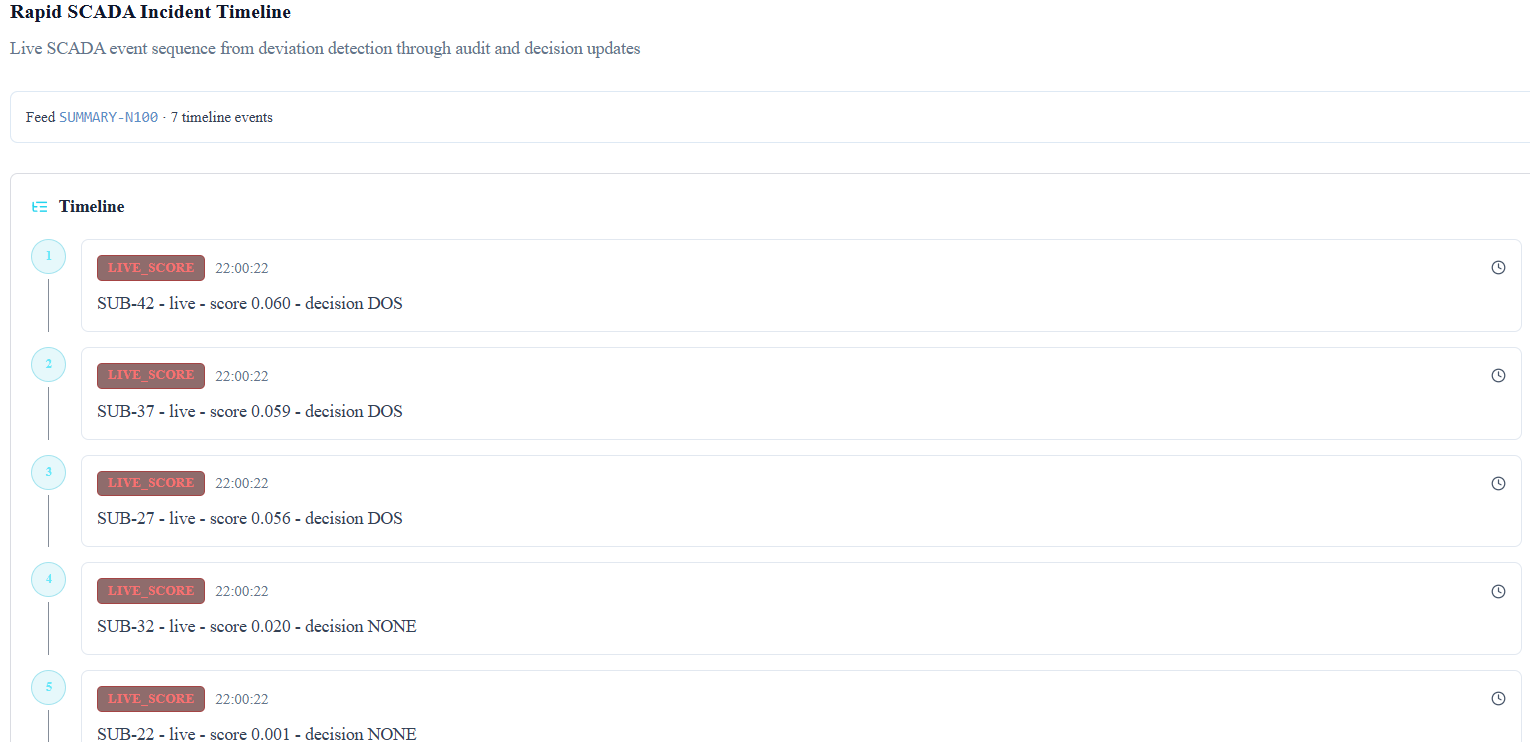
\includegraphics[width=0.95\textwidth]{FigRapid_SCADA_Incident_Timeline.png}}
\caption{Incident timeline view from the SCADA live workspace showing the chronological sequence of detected security events.}
\label{fig:scada_incident_timeline}
\end{figure}

\begin{figure}[H]
\centering
\fbox{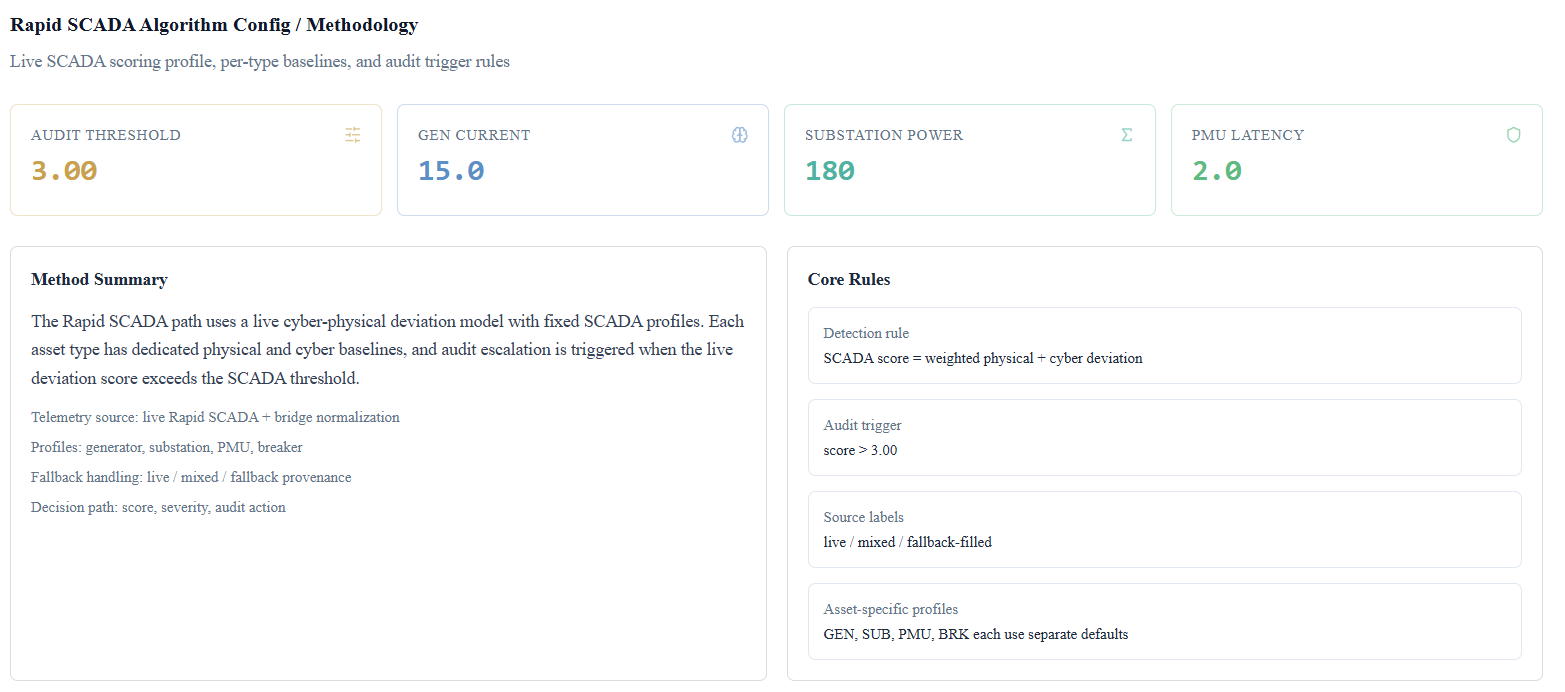
\includegraphics[width=0.95\textwidth]{FigRapid_SCADA_Algorithm_Config_Methodology.png}}
\caption{Algorithm configuration and methodology view from the SCADA live workspace showing the detection pipeline settings.}
\label{fig:scada_algo_config}
\end{figure}

% ============================================================
\section{Operational Workflow}
% ============================================================

The operational workflow of the SmartGrid AI Audit Framework is organised into four sequential phases that correspond to the passage of data through the four architectural tiers.

\par \vspace{0.35cm}
\textbf{Phase I: Data Acquisition.} In the first phase, raw telemetry is acquired from the active data source. In the experiment workspace, data is generated by the backend simulation engine according to the configured scenario parameters. In the SCADA live workspace, data is retrieved from the Rapid SCADA server through the PowerShell bridge. Regardless of source, the raw observations are validated, timestamped, and queued for processing.

\par \vspace{0.35cm}
\textbf{Phase II: Feature Preparation.} In the second phase, each raw observation is decomposed into its physical and cyber feature components. Physical features (voltage, current, frequency, power, response time) and cyber features (latency, packet loss, communication frequency, integrity) are extracted and normalised against their type-specific baselines using the transformation defined in Equation~\ref{eq:normalisation}. The result is a standardised feature vector for each agent at each timestep.

\par \vspace{0.35cm}
\textbf{Phase III: Multi-Layer Anomaly Evaluation.} In the third phase, the normalised feature vectors are processed by the multi-layer detection engine. The statistical deviation scorer computes instantaneous deviation scores. The LSTM temporal detector processes the 24-timestep sliding window to produce calibrated anomaly probabilities. The weighted ensemble fuses these outputs into hybrid confidence values. Simultaneously, the three-layer multi-detector architecture evaluates the agent against the calibrated threshold (Layer~A), the temporal accumulator (Layer~B), and the attack-specific detectors for FDI, DoS, and MITM (Layer~C). The OR-with-precedence combiner produces the final anomaly determination, and the false positive suppression mechanism filters low-confidence detections.

\par \vspace{0.35cm}
\textbf{Phase IV: Hybrid Audit Decision and Output.} In the fourth phase, the detection outputs are consumed by the hybrid audit scheduler, which determines the appropriate audit frequency and escalation action for each agent using Q-learning and gradient-based cost optimisation under budget constraints. The explainability module generates per-agent reason codes and feature contribution rankings. All outputs, anomaly flags, risk scores, escalation actions, and explanations, are pushed to the visualisation layer for operator consumption and are simultaneously logged to the audit trail for traceability.

% ============================================================
\section{Research Contributions}
% ============================================================

The proposed SmartGrid AI Audit Framework makes the following research and engineering contributions:

\begin{enumerate}
    \item \textbf{Unified Cyber-Physical Framework:} A single platform that combines multi-layer anomaly detection, hybrid audit decision support, per-feature explainability, and live SCADA integration within a single modular architecture.

    \item \textbf{Multi-Layer Detection with Ensemble Fusion:} A detection methodology that combines statistical deviation scoring with LSTM-based temporal analysis through a weighted ensemble (deviation weight 0.48, LSTM probability weight 0.52), producing calibrated hybrid confidence estimates.

    \item \textbf{Three-Layer Multi-Detector for Attack Classification:} A specialised detection architecture comprising a calibrated LSTM threshold (Layer~A), a temporal accumulator (Layer~B), and attack-specific detectors for false data injection via CUSUM, denial of service via rule-based corroboration, and man-in-the-middle via integrity-jump analysis (Layer~C).

    \item \textbf{Hybrid Audit Scheduling under Budget Constraints:} A scheduling mechanism that combines Q-learning-based frequency adjustment with gradient-based cost optimisation to determine cost-efficient audit strategies while enforcing operational budget limits.

    \item \textbf{Dual-Workspace Separation:} A clear architectural separation between the experiment evaluation environment and the live operational monitoring environment, so that benchmarking and production monitoring can run independently over a shared detection and audit engine.

    \item \textbf{End-to-End SCADA Telemetry Path:} A fully operational data pipeline from Rapid SCADA through a PowerShell bridge to the FastAPI backend, showing real SCADA-to-backend telemetry acquisition and processing in action.

    \item \textbf{Live 100-Agent Deployment:} A live deployment spanning 100 agents across four distinct asset classes, generators, substations, phasor measurement units, and breakers, each with type-specific baselines and feature definitions.

    \item \textbf{Explainable Scoring with Feature Contribution Ranking:} A per-agent, per-timestep explainability mechanism that computes relative feature contributions independently for physical and cyber domains, producing human-readable reason codes for every detection.

    \item \textbf{Five-Method Comparative Validation Study:} A comparative evaluation of the proposed multi-layer approach against deviation-only, LSTM-only, Isolation Forest, and One-Class SVM baselines, which confirms the value of the ensemble and multi-detector design.

    \item \textbf{From Conceptual Framework to Functioning Platform:} An extension of the foundational base paper from a conceptual cyber-physical audit framework to a fully implemented, integrated, and deployable software platform with real-time monitoring, detection, and decision support capabilities.

    \item \textbf{Five-Class Attack Typing with Temporal Signature Analysis:} An attack classification layer that assigns each flagged agent one of five attack type labels (FDI, DoS, MITM, Physical Fault, and Coordinated Chain Attack) by combining Layer~C detector outputs with a lightweight temporal signature classifier that recognises STEP, RAMP, OSCILLATORY, and STABLE deviation patterns.

    \item \textbf{Dual-Dataset LSTM Pre-Training Pipeline:} A pre-training methodology that initialises the physical grid branch using the UCI Electrical Grid Stability Dataset and the cyber network branch using the UNSW-NB15 Network Intrusion Dataset, with engineered composite features that map directly onto the simulation's cyber feature space. This pre-training step gives each LSTM branch meaningful starting weights before fine-tuning on synthetic grid data.
\end{enumerate}


\chapter{Implementations }
This chapter presents the implementation details of the SmartGrid AI Audit Framework. It covers the system environment and technology stack, the data representation scheme for the 100-agent smart grid, the algorithmic flow of the live detection pipeline, the mathematical formulations behind each computational stage, the integration workflow connecting all subsystems, and the feature-wise functional mapping used throughout the framework. The implementation turns the conceptual framework proposed by Priyadarsini~\cite{priyadarsini2025} into a fully working platform.

%---------------------------------------------------------------------
\section{System Environment and Technology Stack}
\label{sec:tech_stack}
%---------------------------------------------------------------------

The framework is implemented using a modular stack comprising a Python-based backend, a JavaScript-based frontend, a SCADA supervisory layer, a data acquisition bridge, and local storage. All components are executed on a standard workstation without the requirement of a dedicated GPU, making it easy to reproduce and run.

\par \vspace{0.35cm}
\noindent
\textbf{Backend: FastAPI (Python):} The core backend is built using FastAPI, a high-performance Python web framework based on ASGI. It exposes REST endpoints for SCADA data ingestion, anomaly scoring, multi-layer detection, audit scheduling, and explainability (XAI) output. FastAPI was selected for its native support of asynchronous request handling, automatic OpenAPI documentation, and compatibility with the scientific Python ecosystem.

\par \vspace{0.35cm}
\noindent
\textbf{Frontend: Next.js Dashboard:} The operator-facing interface is implemented as a Next.js application (React-based framework). The dashboard is organised into two distinct workspaces:
\begin{itemize}
    \item \textit{Experiment Running}, used for simulation, benchmarking, and comparative evaluation of detection methods.
    \item \textit{Rapid SCADA Live}, used for real-time monitoring of the 100-agent grid, displaying live telemetry, anomaly flags, audit decisions, and explainability outputs.
\end{itemize}

\par \vspace{0.35cm}
\noindent
\textbf{SCADA Layer: Rapid SCADA:} Rapid SCADA Webstation serves as the supervisory telemetry layer~\cite{martinelli2022method}. The Rapid SCADA Web API, accessible at \texttt{127.0.0.1:10109}, provides authenticated access to channel data. A total of 670 calculated channels are configured across two configuration files, \texttt{Cnl.xml} for physical channels and \mbox{\texttt{Cnl\_Cyber\_Addon.xml}} for cyber channels, to represent the telemetry of the 100-agent grid. Generators use channels 101--160 (physical) and 501--580 (cyber), substations use 201--290 and 601--690, PMUs use 301--375 and 701--800, and breakers use 401--475 and 801--900. Calculated channels were used rather than input channels because input channels in Rapid SCADA require physical device connections, whereas calculated channels allow programmatic generation of telemetry values within the SCADA environment.

\par \vspace{0.35cm}
\noindent
\textbf{Data Acquisition Bridge: PowerShell Script:} A PowerShell script serves as the bridge between Rapid SCADA and the FastAPI backend. The bridge script (\mbox{\texttt{pull\_rapidscada\_to\_api.ps1}}) authenticates with the Rapid SCADA Web API, retrieves telemetry values in batch, and transmits them to the backend ingestion endpoint~\cite{martinelli2022method}. This approach decouples the SCADA layer from the backend, allowing independent operation and testing of each component.

\par \vspace{0.35cm}
\noindent
\textbf{Machine Learning: PyTorch:} All LSTM-based temporal detection models are implemented using PyTorch. The dual-branch LSTM architecture (grid branch and network branch) is trained and executed entirely within the Python backend. PyTorch was chosen for its dynamic computation graph, ease of debugging, and compatibility with the rest of the Python stack.

\par \vspace{0.35cm}
\noindent
\textbf{Database: SQLite:} SQLite is used for persistent storage of the audit chain and telemetry records. The audit chain database (\texttt{audit\_chain.db}) stores all audit decisions, anomaly flags, risk scores, and scheduling outcomes. SQLite was selected for its zero-configuration deployment, single-file storage, and suitability for single-machine operation without a dedicated database server.

\par \vspace{0.35cm}
\noindent
\textbf{Execution Environment:} The entire framework operates on a standard workstation. No GPU acceleration is required for inference or training at the current 100-agent scale. This design choice ensures that the system can be reproduced and evaluated without specialised hardware.

\begin{figure}[H]
\centering
\fbox{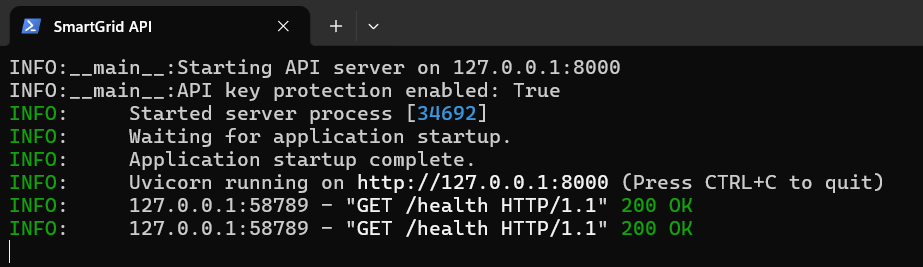
\includegraphics[width=0.95\textwidth]{SmartGridAPI.png}}
\caption{FastAPI backend running with all REST endpoints for SCADA ingestion, anomaly detection, audit scheduling, and explainability.}
\label{fig:smartgrid_api}
\end{figure}

\begin{figure}[H]
\centering
\fbox{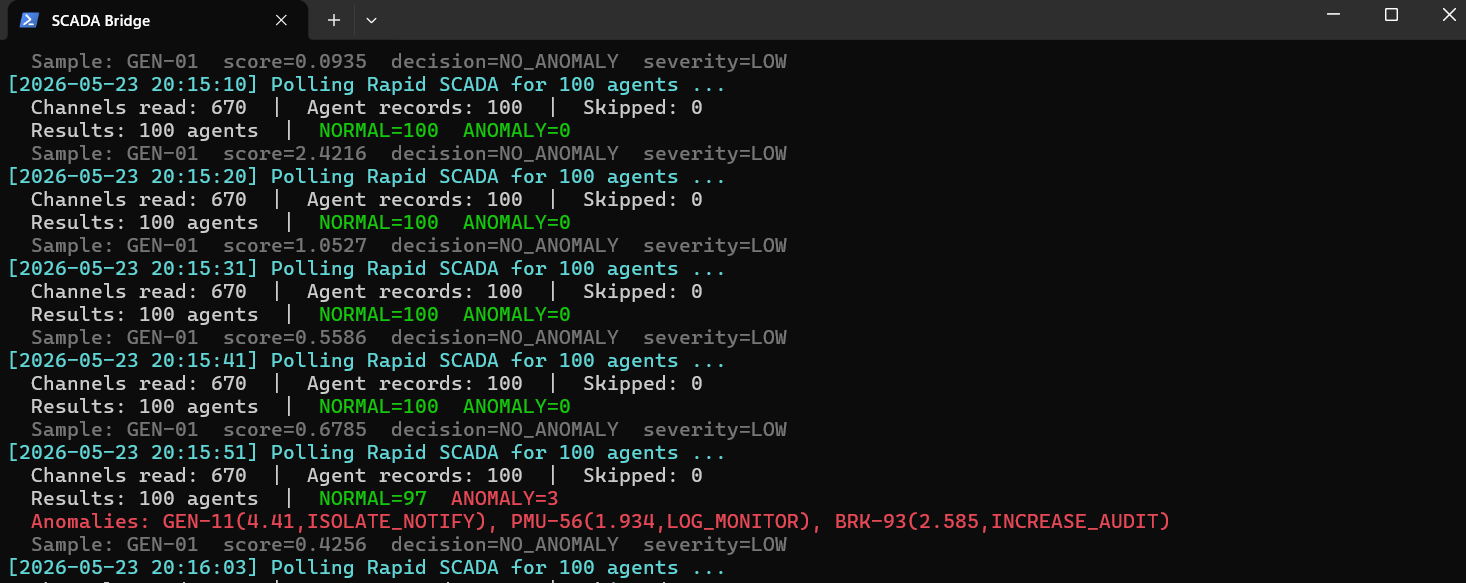
\includegraphics[width=0.95\textwidth]{SCADABridge_Terminal.png}}
\caption{PowerShell bridge terminal showing live telemetry retrieval from Rapid SCADA and batch transmission to the FastAPI backend.}
\label{fig:scada_bridge_terminal}
\end{figure}


%---------------------------------------------------------------------
\section{Smart Grid Data Representation}
\label{sec:data_representation}
%---------------------------------------------------------------------

The smart grid is modelled as a multi-agent system~\cite{farid2014multi} comprising 100 agents distributed across four functional classes. Each agent is assigned a unique identifier and a set of physical and cyber features that collectively characterise its operational state. All telemetry data used in both the experiment and SCADA live workspaces is synthetically generated: the experiment workspace uses the \texttt{GridEnvConfig}-based simulation engine (\texttt{grid\_env.py}), while the SCADA live workspace uses calculated channels within Rapid SCADA that produce programmatically generated values. No external or third-party datasets are used as the live or simulation telemetry source. However, two public benchmark datasets, the UCI Electrical Grid Stability Dataset and the UNSW-NB15 Network Intrusion Dataset, are used exclusively for LSTM model pre-training prior to fine-tuning on the synthetic grid data. This distinction is important: the datasets train the model weights, not the runtime telemetry pipeline (see Section~\ref{sec:lstm_arch_training}).

\par \vspace{0.35cm}
\noindent
\textbf{Agent Classes and Identifiers:} The 100 agents are organised into four classes as follows:
\begin{itemize}
    \item \textbf{Generators (GEN):} GEN-01 to GEN-20 (20 agents), represent power generation units.
    \item \textbf{Substations (SUB):} SUB-21 to SUB-50 (30 agents), represent power transformation and distribution nodes.
    \item \textbf{Phasor Measurement Units (PMU):} PMU-51 to PMU-75 (25 agents), represent high-frequency synchronised measurement devices.
    \item \textbf{Breakers (BRK):} BRK-76 to BRK-100 (25 agents), represent circuit protection and switching devices.
\end{itemize}

\par \vspace{0.35cm}
\noindent
\textbf{Physical Features:} Each agent reports a set of physical measurements that reflect the electrical state of the corresponding grid component. The physical feature vector $\mathbf{x} \in \mathbb{R}^{n_x}$ includes:
\begin{itemize}
    \item \textit{Voltage} (in volts), bus voltage magnitude (nominal 230\,V for generators).
    \item \textit{Current} (in amperes), line current magnitude (nominal 100\,A for generators).
    \item \textit{Frequency} (in hertz), system frequency at the measurement point (nominal 50\,Hz).
    \item \textit{Power} (in kilowatts), active power flow (derived from voltage $\times$ current $\times$ power factor).
    \item \textit{Response Time} (in milliseconds), measurement response latency of the physical sensor.
\end{itemize}

\par \vspace{0.35cm}
\noindent
\textbf{Cyber Features:} Each agent additionally reports a set of cyber (network) measurements that characterise the communication health of its telemetry channel. The cyber feature vector $\mathbf{y} \in \mathbb{R}^{n_y}$ includes:
\begin{itemize}
    \item \textit{Latency} (in milliseconds), round-trip communication delay.
    \item \textit{Packet Loss} (as a ratio), fraction of telemetry packets lost in transit.
    \item \textit{Communication Frequency} (in hertz), rate of telemetry reporting.
    \item \textit{Integrity} (as a score), computed integrity metric for the communication channel.
\end{itemize}

\par \vspace{0.35cm}
\noindent
\textbf{Rapid SCADA Channel Model:} The 100-agent grid is represented within Rapid SCADA using a total of 670 calculated channels distributed across physical and cyber configuration files. The channel allocation varies by asset class: generators receive 7 channels each (3 physical + 4 cyber), substations receive 6 channels each (3 physical + 3 cyber, with no dedicated cyber latency channel), PMUs receive 7 channels each (3 physical + 4 cyber), and breakers receive 7 channels each (3 physical + 4 cyber). As noted in Section~\ref{sec:tech_stack}, calculated channels were used in place of input channels because input channels in Rapid SCADA require connections to physical field devices, which are not present in the current deployment. Calculated channels allow the SCADA environment to generate representative telemetry values programmatically, which allows full pipeline validation without hardware dependencies.

\par \vspace{0.35cm}

\begin{figure}[H]
\centering
\fbox{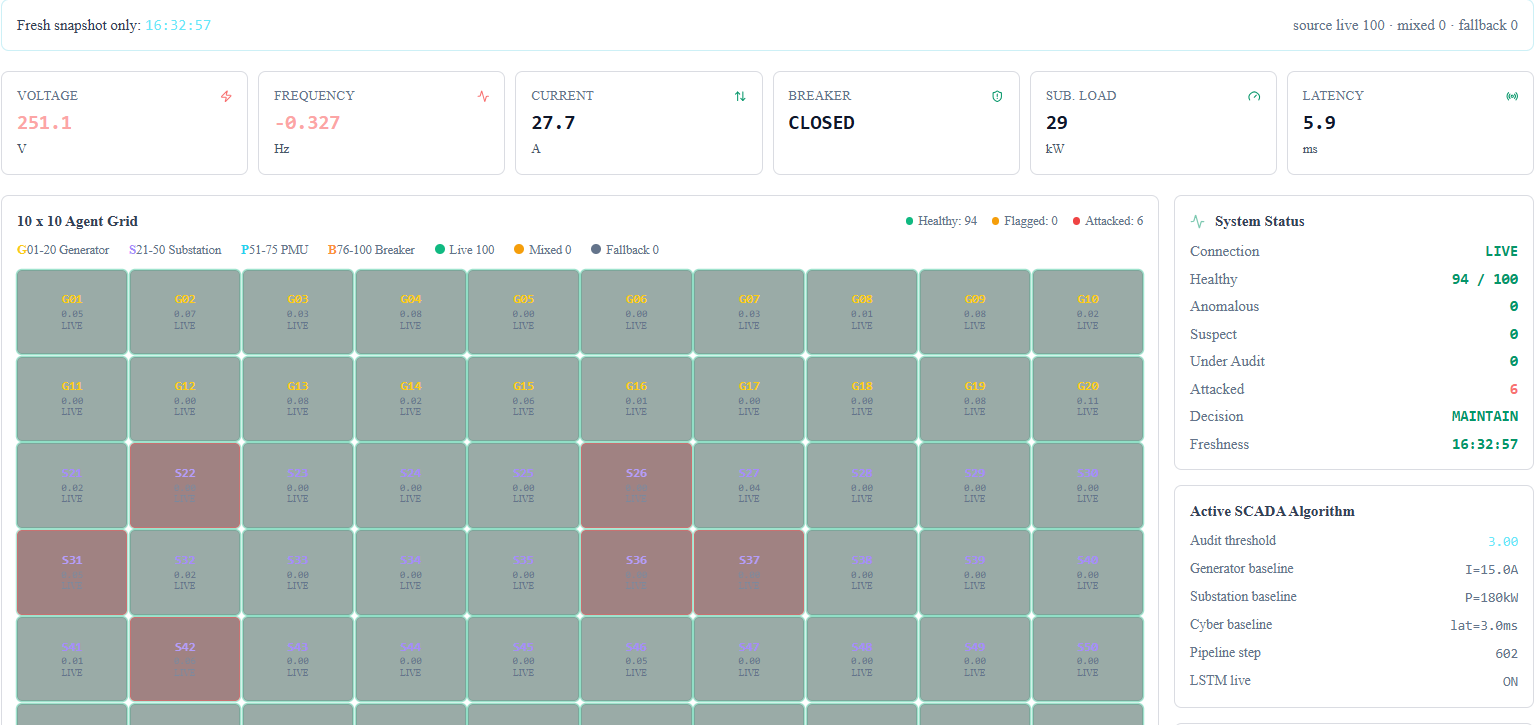
\includegraphics[width=0.95\textwidth]{FigGrid_With_The_Agents.png}}
\caption{Rapid SCADA live grid view showing the 100-agent smart grid with generators, substations, PMUs, and breakers.}
\label{fig:grid_agents}
\end{figure}

\begin{figure}[H]
\centering
\fbox{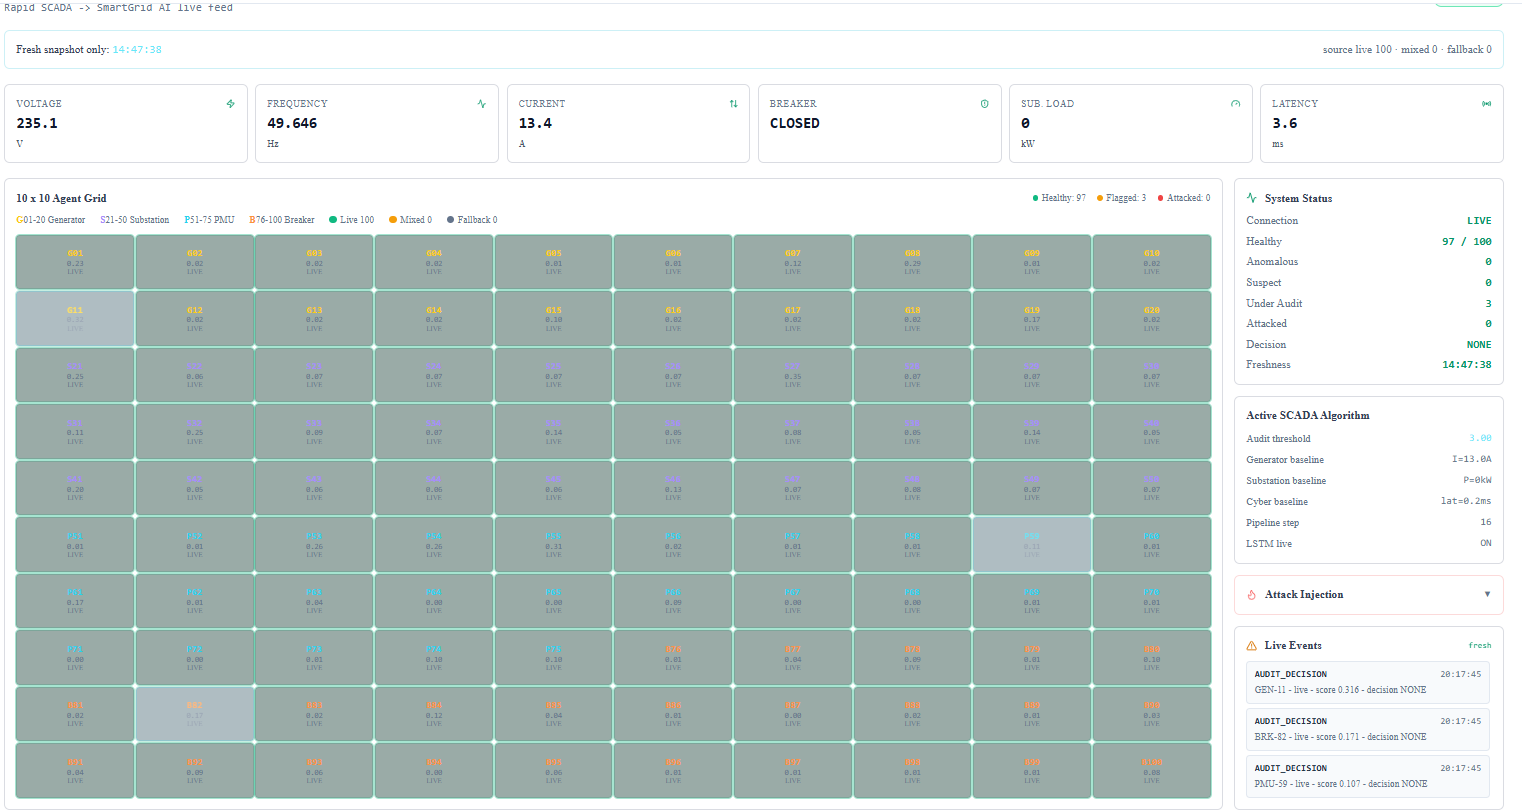
\includegraphics[width=0.95\textwidth]{FigScadaGrid_Normal.png}}
\caption{SCADA grid view during normal operation showing all agents in healthy state with no anomaly flags.}
\label{fig:scada_grid_normal}
\end{figure}

\begin{figure}[H]
\centering
\fbox{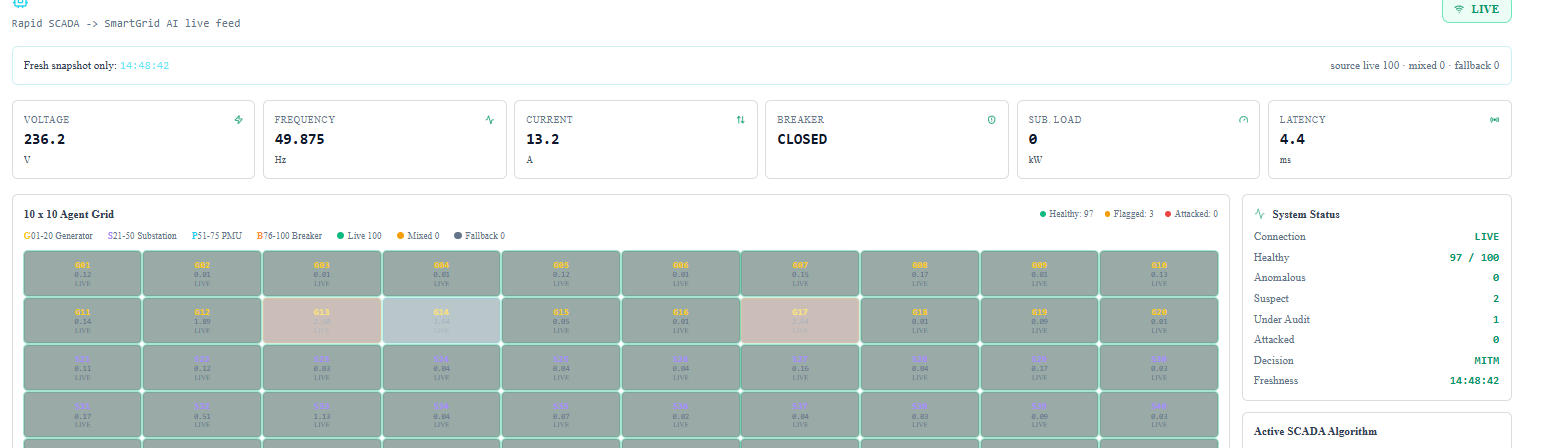
\includegraphics[width=0.95\textwidth]{FigScadaGrid_Attack.png}}
\caption{SCADA grid view during an active attack scenario showing affected agents flagged with anomaly indicators.}
\label{fig:scada_grid_attack}
\end{figure}


%---------------------------------------------------------------------
\section{Algorithmic Flow and Execution Process}
\label{sec:algo_flow}
%---------------------------------------------------------------------

The live detection pipeline follows a nine-step sequential process. Each step transforms or enriches the data, progressing from raw telemetry acquisition to final operator-facing outputs. The steps are described below.

\par \vspace{0.35cm}
\noindent
\textbf{Step 1: Data Acquisition:} Telemetry data is acquired from one of two sources depending on the active workspace. In the \textit{Experiment Running} workspace, data is generated or loaded from simulation datasets. In the \textit{Rapid SCADA Live} workspace, the PowerShell bridge (\mbox{\texttt{pull\_rapidscada\_to\_api.ps1}}) retrieves telemetry from the Rapid SCADA Web API at \texttt{127.0.0.1:10109} and transmits it to the FastAPI backend in batch form. This step produces the raw physical feature vector $\mathbf{x}$ and cyber feature vector $\mathbf{y}$ for each agent.

\par \vspace{0.35cm}
\noindent
\textbf{Step 2: Observation:} Each agent executes an observation step via the method \texttt{agent.observe($\mathbf{x}_{\text{phys}}$, $\mathbf{y}_{\text{cyber}}$)}. This method registers the incoming physical and cyber feature vectors into the agent's internal state, making them available for subsequent scoring and detection operations. The observation step also updates the agent's telemetry history buffer, which is used by the LSTM temporal model.

\par \vspace{0.35cm}
\noindent
\textbf{Step 3: LSTM Inference:} A dual-branch LSTM model processes the agent's recent telemetry history. The grid branch analyses physical features to produce a grid anomaly probability, while the network branch analyses cyber features to produce a network intrusion probability. The two branch outputs are combined using the function \mbox{\texttt{fuse\_branch\_probabilities()}} with fusion weights $w_{\text{grid}} = 0.58$ and $w_{\text{network}} = 0.42$, yielding a unified anomaly probability $p_{\text{anomaly}} \in [0,1]$. This picks up patterns that instantaneous deviation scoring alone would miss.

\par \vspace{0.35cm}
\noindent
\textbf{Step 4: Scoring:} The function \texttt{compute\_score\_and\_flag()} calculates the agent's composite risk score and binary anomaly flag. This step proceeds as follows:
\begin{enumerate}
    \item \textit{EWMA Drift Compensation:} Before deviation scoring, a slow drift correction is applied to prevent the scorer from raising false alarms during gradual but legitimate load shifts. An exponentially weighted moving average (EWMA) with smoothing factor $\alpha_{\text{ewma}} = 0.30$ tracks the rolling mean of each feature over a window of 24 timesteps. When the rolling mean drifts from the static baseline by more than a marginal amount, 30\% of that difference is subtracted from the observed value prior to computing the normalised deviation. This keeps the effective deviation centred on the true short-term operating point rather than the fixed installation-time baseline.
    \item \textit{Deviation Scoring:} The physical deviation $d_x$ and cyber deviation $d_y$ are computed as the root-mean-square of the EWMA-compensated normalised feature deviations from the agent's baseline (see Equations~\ref{eq:dx} and~\ref{eq:dy}). The composite score is $S_i(t) = w_i \cdot (d_x + d_y)$, where $w_i$ is the agent's criticality weight (Equation~\ref{eq:si}).
    \item \textit{Weighted Ensemble:} The hybrid confidence score combines deviation-based and LSTM-based evidence:
    \begin{equation}
    \text{hybrid\_conf} = 0.48 \cdot \text{dev\_conf} + 0.52 \cdot \text{prob\_support} + \text{suspicion\_credit}
    \label{eq:hybrid_inline}
    \end{equation}
    where the weights 0.48 and 0.52 reflect the validated configuration giving slightly greater emphasis to the temporal LSTM detector.
    \item \textit{Binary Flag:} The anomaly flag $a_i(t)$ is set to 1 if the combined conditions on deviation magnitude and hybrid confidence exceed the agent's calibrated thresholds, and 0 otherwise.
\end{enumerate}

\par \vspace{0.35cm}
\noindent
\textbf{Detection Sensitivity Profiles.} The system supports three named runtime profiles that adjust the primary detection thresholds without retraining any model component. Each profile trades sensitivity against false positive tolerance according to operational requirements:

\begin{itemize}
    \item \textit{ROBUST}, $k_\sigma = 3.5$, deviation score threshold $= 3.60$, LSTM probability threshold $= 0.80$. This profile is the most sensitive and is suited for high-security environments where the cost of a missed attack outweighs the nuisance of occasional false alarms.
    \item \textit{BALANCED}, $k_\sigma = 4.0$, deviation score threshold $= 3.85$, LSTM probability threshold $= 0.85$. This is the default operational profile and provides the best overall F1 score across the evaluated scenarios.
    \item \textit{COST}, $k_\sigma = 5.0$, deviation score threshold $= 4.10$, LSTM probability threshold $= 0.90$. This profile minimises audit expenditure by raising the evidence bar for flagging an agent, and is appropriate when audit resources are constrained and the expected attack rate is low.
\end{itemize}

The $k_\sigma$ parameter scales the adaptive threshold used in the sigma-window computation, where the threshold for each feature is $\tau = k_\sigma \cdot \hat{\sigma}$ and $\hat{\sigma}$ is the empirical standard deviation over the most recent 24-timestep window.

\par \vspace{0.35cm}
\noindent
\textbf{Step 5: Multi-Layer Detection:} A three-layer detection architecture provides defence in depth:
\begin{enumerate}
    \item \textbf{Layer 1: Calibrated LSTM Threshold:} The LSTM anomaly probability is compared against a calibrated per-agent threshold. Agents whose $p_{\text{anomaly}}$ exceeds the threshold are flagged at this layer.
    \item \textbf{Layer 2: Temporal Accumulator:} A sliding-window accumulator tracks the frequency of anomaly flags over recent time steps. Agents exhibiting sustained anomalous behaviour (i.e., repeated flags within the accumulation window) are escalated, even if individual flags are marginally above the threshold.
    \item \textbf{Layer 3: Specialised Attack Detectors:} Four attack-specific detectors operate in parallel:
    \begin{itemize}
        \item \textit{CUSUM Detector}, for false data injection (FDI) attacks~\cite{liu2009false}, based on cumulative sum change-point detection on physical feature residuals, with a shape gate that requires the latest residual to match the FDI pattern before the detector fires.
        \item \textit{DoS Detector}, for denial-of-service attacks, based on rule-based evaluation of communication frequency drops and packet loss spikes.
        \item \textit{MITM Detector}, for man-in-the-middle attacks, based on integrity score degradation and latency anomalies.
        \item \textit{Fault Signature Detector}, for physical faults (voltage sag, overcurrent, and frequency deviation), based on template matching when one physical feature stands out while the cyber channels stay quiet. This detector takes precedence over the CUSUM detector when both fire, so a fault is not mislabelled as an FDI attack.
    \end{itemize}
    A cross-layer corroboration check then drops a deviation-only flag when neither the LSTM nor any of the four detectors agrees with it, which lowers the false alarm rate.
\end{enumerate}

\par \vspace{0.35cm}
\noindent
\textbf{Step 6: Behaviour Update:} After detection, each agent refines its internal baseline and detection thresholds. Baseline values are updated using an exponential moving average with smoothing factor $\alpha = 0.1$, applied \textit{only when the anomaly flag is zero} (i.e., during normal conditions). During detected anomalies, baselines are frozen to prevent contamination from attack-corrupted observations. This guard ensures that sustained attacks cannot gradually shift the baseline toward malicious values. Detection thresholds are adjusted based on the observed false positive rate and detection sensitivity, so that the system stays calibrated over time.

\par \vspace{0.35cm}
\noindent
\textbf{Step 7: Audit Scheduling:} The hybrid audit scheduler determines the audit frequency for each agent using two complementary mechanisms:
\begin{itemize}
    \item \textit{Reinforcement Learning (Q-Learning):} A Q-table maps agent risk states to audit frequency actions. The Q-values are updated after each audit decision based on the observed reward, which balances detection effectiveness against audit cost.
    \item \textit{Gradient-Based Cost Optimisation:} The audit frequency is further refined by minimising a cost function that balances audit cost against expected risk exposure. The gradient of this cost function with respect to audit frequency is computed analytically and used to update the frequency through gradient descent (see Section~\ref{sec:gradient_audit}).
\end{itemize}
The function \texttt{hybrid\_audit\_schedule()} combines the outputs of both mechanisms to produce the final audit frequency for each agent.

\par \vspace{0.35cm}
\noindent
\textbf{Step 8: Response and Action Escalation:} Based on the detection results and audit decisions, the system selects one of five escalation levels for each agent:
\begin{itemize}
    \item \texttt{NO\_ANOMALY}, normal operation; no action required.
    \item \texttt{LOG\_MONITOR}, marginal deviation; event is logged and passive monitoring is enhanced.
    \item \texttt{INCREASE\_AUDIT}, elevated monitoring; audit frequency is increased.
    \item \texttt{ISOLATE\_NOTIFY}, the agent is flagged for isolation and the operator is notified.
    \item \texttt{EMERGENCY\_SHUTDOWN}, critical threat; immediate shutdown action is recommended.
\end{itemize}

\par \vspace{0.35cm}
\noindent
\textbf{Step 9: XAI Output:} The explainability module invokes \texttt{explain\_deviation()} independently for physical and cyber feature domains. For each domain, the module computes per-feature contribution scores (see Section~\ref{sec:xai_formulas}) and identifies the top contributing features driving the anomaly flag. The output is a ranked list of features with their relative contributions, presented to the operator through the dashboard.

\begin{figure}[H]
\centering
\fbox{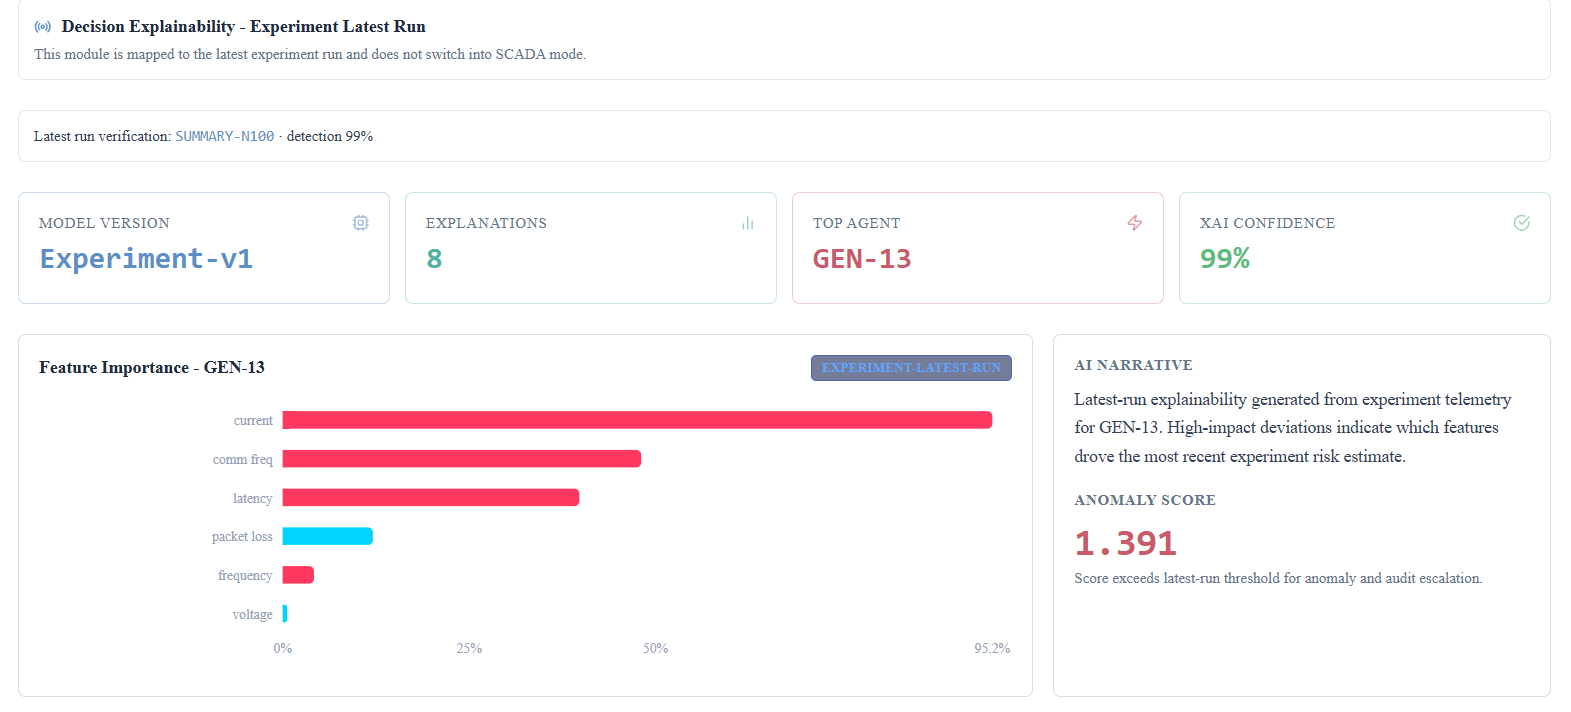
\includegraphics[width=0.95\textwidth]{FigExperiment_Decision_Explainability.png}}
\caption{Explainability (XAI) view showing per-feature deviation contributions for a selected agent, with physical and cyber domains displayed independently.}
\label{fig:xai_view}
\end{figure}


%---------------------------------------------------------------------
\section{Mathematical Formulations}
\label{sec:math_formulations}
%---------------------------------------------------------------------

This section presents the mathematical formulations underlying the key computational stages of the framework. All equations use consistent notation: $\mathbf{x}$ denotes physical features, $\mathbf{y}$ denotes cyber features, $\mathbf{b}$ denotes baseline values, and $\boldsymbol{\theta}$ denotes threshold values.

%.....................................................................
\subsection{Deviation Scoring Formulas}
\label{sec:deviation_formulas}
%.....................................................................

The deviation scoring module, adapted from the formulation in~\cite{priyadarsini2025}, quantifies how far an agent's current observations deviate from its learned baseline. The normalised z-score for a single feature observation is defined as:
\begin{equation}
z = \frac{\text{obs} - \text{base}}{\theta}
\label{eq:z}
\end{equation}
where $\text{obs}$ is the observed value, $\text{base}$ is the baseline value, and $\theta$ is the corresponding threshold.

\par \vspace{0.25cm}
\noindent
The physical deviation $d_x$ aggregates the normalised deviations across all physical features:
\begin{equation}
d_x = \sqrt{ \frac{1}{n_x} \sum_{j=1}^{n_x} \left( \frac{x_j - b_{x,j}}{\theta_{x,j}} \right)^2 }
\label{eq:dx}
\end{equation}
where $n_x$ is the number of physical features, $x_j$ is the observed value of the $j$-th physical feature, $b_{x,j}$ is its baseline, and $\theta_{x,j}$ is its threshold.

\par \vspace{0.25cm}
\noindent
Similarly, the cyber deviation $d_y$ is computed over all cyber features:
\begin{equation}
d_y = \sqrt{ \frac{1}{n_y} \sum_{j=1}^{n_y} \left( \frac{y_j - b_{y,j}}{\theta_{y,j}} \right)^2 }
\label{eq:dy}
\end{equation}
where $n_y$ is the number of cyber features, $y_j$ is the observed value of the $j$-th cyber feature, $b_{y,j}$ is its baseline, and $\theta_{y,j}$ is its threshold.

\par \vspace{0.25cm}
\noindent
The composite deviation score for agent $i$ at time $t$ is:
\begin{equation}
S_i(t) = w_i \cdot (d_x + d_y)
\label{eq:si}
\end{equation}
where $w_i$ is the criticality weight assigned to agent $i$ based on its class (generator, substation, PMU, or breaker).

%.....................................................................
\subsection{LSTM Ensemble and Hybrid Confidence}
\label{sec:hybrid_confidence}
%.....................................................................

The hybrid confidence score combines evidence from the deviation-based detector and the LSTM-based temporal detector using a weighted ensemble:
\begin{equation}
\text{hybrid\_conf} = w_{\text{dev}} \cdot \text{dev\_conf} + w_{\text{prob}} \cdot \text{prob\_support} + \text{suspicion\_credit}
\label{eq:hybrid}
\end{equation}
where $w_{\text{dev}} = 0.48$ is the deviation confidence weight, $w_{\text{prob}} = 0.52$ is the LSTM probability weight, $\text{dev\_conf}$ is the confidence derived from deviation magnitude, $\text{prob\_support}$ is the LSTM anomaly probability, and $\text{suspicion\_credit}$ is an additional term accumulated from the temporal accumulator when sustained anomalous behaviour is observed.

\par \vspace{0.25cm}
\noindent
The binary anomaly flag for agent $i$ at time $t$ is determined as:
\begin{equation}
a_i(t) =
\begin{cases}
1, & \text{if the combined conditions on deviation magnitude and} \\
   & \text{hybrid confidence exceed the calibrated thresholds} \\
0, & \text{otherwise}
\end{cases}
\label{eq:ai}
\end{equation}

%.....................................................................
\subsection{LSTM Architecture and Training Methodology}
\label{sec:lstm_arch_training}
%.....................................................................

\textbf{Model Architecture.} Each branch of the dual-branch LSTM is a two-layer LSTM with 64 hidden units per layer and a dropout of 0.20 between layers. A single fully-connected output layer maps the last hidden state to one logit, and a sigmoid activation converts that logit to a probability in $[0,1]$. Temporal input sequences are formed by a sliding window of 24 consecutive timesteps, giving each training sample the shape $(24,\, n_{\text{feat}})$. The window size of 24 captures one short-term operational cycle at the standard SCADA polling interval and was validated to provide stable gradient flow without overfitting. The data is split 80\% for training and 20\% for validation. Training uses the Adam optimiser at a learning rate of $10^{-3}$, a batch size of 64, and runs for up to 20 epochs.

\par \vspace{0.35cm}
\noindent
\textbf{Pre-Training Datasets.} The dual-branch LSTM is pre-trained on two publicly available benchmark datasets before fine-tuning on the synthetic grid simulation data. The pre-training step gives each branch a meaningful starting point that reflects real-world physical and network dynamics, reducing the amount of synthetic data needed to reach convergence.

\par \vspace{0.25cm}
\noindent
\textit{UCI Electrical Grid Stability Dataset (Dataset \#471).} The physical grid branch is pre-trained on the UCI Electrical Grid Stability Dataset, which contains 10{,}000 samples with 12 numerical features: four producer reaction times (\texttt{tau1}--\texttt{tau4}), four power balance coefficients (\texttt{p1}--\texttt{p4}), and four price elasticity coefficients (\texttt{g1}--\texttt{g4}). The binary stability label (stable / unstable) serves as the pre-training target. The continuous regression column \texttt{stab} is excluded, and any missing values are filled using per-feature median imputation. The dataset models a four-node power network under varying supply-demand conditions, which means the physical branch learns the characteristic dynamics of voltage and frequency imbalance before it ever sees a smart grid observation. Table~\ref{tab:uci_feature_map} shows how the UCI feature groups map onto the physical features of the grid simulation.

\begin{table}[H]
\centering
\caption{UCI Electrical Grid Stability Dataset: feature-to-simulation mapping.}
\label{tab:uci_feature_map}
\begin{tabular}{|l|l|l|}
\hline
\textbf{UCI Feature Group} & \textbf{UCI Columns} & \textbf{Simulation Mapping} \\
\hline
Producer reaction times & \texttt{tau1}--\texttt{tau4} & Physical response latency \\
Power balance & \texttt{p1}--\texttt{p4} & Voltage and power deviations \\
Price elasticity & \texttt{g1}--\texttt{g4} & Frequency and current load sensitivity \\
\hline
\end{tabular}
\end{table}

\par \vspace{0.25cm}
\noindent
\textit{UNSW-NB15 Network Intrusion Dataset.} The network/cyber branch is pre-trained on the UNSW-NB15 dataset. Rather than feeding in the raw 47-feature vector, four composite engineered features are derived that correspond one-to-one with the four cyber features used in the simulation:

\begin{enumerate}
    \item $\text{latency\_like} = \ln\!\left(1 + \texttt{dur} + \texttt{tcprtt} + \texttt{synack} + \texttt{ackdat} + \texttt{sinpkt} + \texttt{dinpkt} + \texttt{sjit} + \texttt{djit}\right)$
    \item $\text{loss\_like} = \ln\!\left(1 + \texttt{sloss} + \texttt{dloss} + \text{pkt\_correction}\right)$
    \item $\text{integrity\_like} = \ln\!\left(1 + |\texttt{sttl} - \texttt{dttl}| + \texttt{ct\_state\_ttl} + \tfrac{|\texttt{sbytes} - \texttt{dbytes}|}{\max(\texttt{sbytes}+\texttt{dbytes},\, 1)}\right)$
    \item $\text{freq\_like} = \ln\!\left(1 + \texttt{rate} + \texttt{sload} + \texttt{dload} + \texttt{spkts} + \texttt{dpkts}\right)$
\end{enumerate}

The $\ln(1+x)$ transform compresses the heavy-tailed distributions typical of network flow data. Each composite is then z-score normalised across the dataset. The mapping is deliberate: \textit{latency\_like} aggregates timing and inter-packet gap signals, mapping to the \textit{latency} cyber feature; \textit{loss\_like} captures retransmission and packet drop patterns, mapping to \textit{packet loss}; \textit{integrity\_like} reflects header discrepancies and data consistency deviations, mapping to \textit{integrity}; and \textit{freq\_like} captures throughput and rate, mapping to \textit{communication frequency}. The binary label (\texttt{label} $> 0$ = attack) trains the cyber branch to distinguish normal network flows from intrusion patterns. Table~\ref{tab:unsw_feature_map} summarises the correspondence.

\begin{table}[H]
\centering
\caption{UNSW-NB15 engineered features and their cyber feature mappings.}
\label{tab:unsw_feature_map}
\begin{tabular}{|l|l|l|}
\hline
\textbf{Engineered Feature} & \textbf{Source Fields (UNSW-NB15)} & \textbf{Simulation Cyber Feature} \\
\hline
\textit{latency\_like} & \texttt{dur, tcprtt, synack, ackdat, sinpkt, dinpkt, sjit, djit} & Latency \\
\textit{loss\_like} & \texttt{sloss, dloss}, packet mismatch & Packet Loss \\
\textit{integrity\_like} & \texttt{sttl, dttl, ct\_state\_ttl, sbytes, dbytes} & Integrity \\
\textit{freq\_like} & \texttt{rate, sload, dload, spkts, dpkts} & Communication Frequency \\
\hline
\end{tabular}
\end{table}

\par \vspace{0.35cm}
\noindent
\textbf{Handling Class Imbalance.} Attack events are rare relative to normal operating time, so training data is skewed heavily toward the negative class. Two techniques are combined to address this. \textit{Focal Loss} replaces standard binary cross-entropy as the training objective:
\begin{equation}
\mathcal{L}_{\text{focal}} = -\alpha \left(1 - p_t\right)^{\gamma} \log(p_t)
\label{eq:focal}
\end{equation}
where $p_t$ is the model's estimated probability for the ground-truth class, $\alpha = 0.65$ is the class weight assigned to the positive (attack) class, and $\gamma = 2.0$ is the focusing exponent. The factor $(1 - p_t)^\gamma$ reduces the loss contribution from easy well-classified samples and concentrates the gradient on harder minority-class examples. Alongside Focal Loss, a \textit{WeightedRandomSampler} oversamples the minority class during batch construction using a positive-class scale factor of 1.40 and an oversampling scale of 1.35, so attack samples appear more frequently within each mini-batch.

\par \vspace{0.35cm}
\noindent
\textbf{Temperature Calibration.} Raw LSTM output probabilities are often poorly calibrated: a predicted value of 0.80 does not necessarily correspond to an 80\% empirical likelihood of attack. After training, a post-hoc temperature calibration step is performed on the held-out validation set. A temperature parameter $T$ is selected by grid search over $T \in [0.80,\, 2.20]$ in increments of 0.05, simultaneously with a decision threshold search over $[0.40,\, 0.65]$. The pair $(T^*, \text{threshold}^*)$ that jointly maximises the validation F1 score and minimises the Brier score (a calibration loss) is saved in the model checkpoint. During inference, the raw logit $z$ is divided by $T^*$ before the sigmoid activation, producing a calibrated probability that is well-suited for its 0.52-weighted contribution to the hybrid confidence ensemble in Equation~\ref{eq:hybrid}.

%.....................................................................
\subsection{Explainability Formulas}
\label{sec:xai_formulas}
%.....................................................................

The explainability module computes per-feature contribution scores to identify which features are most responsible for a given anomaly flag. For each feature $j$ in the physical domain, the squared normalised contribution is:
\begin{equation}
c_j = \left( \frac{x_j - b_j}{\theta_j} \right)^2
\label{eq:cj}
\end{equation}

\par \vspace{0.25cm}
\noindent
The relative contribution of feature $j$ is then:
\begin{equation}
\text{relative}_j = \frac{c_j}{\displaystyle\sum_{k=1}^{n} c_k}
\label{eq:rel}
\end{equation}
where $n$ is the total number of features in the domain. An analogous computation is performed for cyber features using $\mathbf{y}$, $\mathbf{b}_y$, and $\boldsymbol{\theta}_y$. The features with the highest relative contributions are reported in ranked order as the explanation for the anomaly flag.

%.....................................................................
\subsection{Gradient Audit Optimisation}
\label{sec:gradient_audit}
%.....................................................................

The gradient-based audit optimisation module determines the optimal audit frequency for each agent by minimising a cost function that balances audit expenditure against risk exposure. The cost function for agent $i$ is:
\begin{equation}
C_i = C_a \cdot f_i + C_f \cdot \frac{R_i}{f_i}
\label{eq:ci}
\end{equation}
where $C_a$ is the per-audit cost, $f_i$ is the audit frequency for agent $i$, $C_f$ is the penalty cost for undetected risk, and $R_i$ is the estimated risk score for agent $i$. The first term represents the direct cost of conducting audits, while the second term represents the expected cost of risk exposure that decreases with higher audit frequency.

\par \vspace{0.25cm}
\noindent
The gradient of the cost function with respect to audit frequency is:
\begin{equation}
\frac{\partial C_i}{\partial f_i} = C_a - C_f \cdot \frac{R_i}{f_i^2}
\label{eq:grad}
\end{equation}

\par \vspace{0.25cm}
\noindent
The audit frequency is updated iteratively using gradient descent:
\begin{equation}
f_i \leftarrow f_i - \eta \cdot \frac{\partial C_i}{\partial f_i}
\label{eq:update}
\end{equation}
where $\eta = 0.01$ is the gradient learning rate. The update rule decreases the audit frequency when audit cost dominates and increases it when risk exposure dominates, converging to the cost-optimal audit rate for each agent.

%.....................................................................
\subsection{Reinforcement Learning}
\label{sec:rl}
%.....................................................................

The reinforcement learning component of the hybrid audit scheduler employs Q-learning~\cite{priyadarsini2025,ibrahim2023security} to map agent risk states to audit frequency actions. The Q-value update rule is:
\begin{equation}
Q(s, a) \leftarrow Q(s, a) + \alpha \left[ r + \gamma \cdot \max_{a'} Q(s', a') - Q(s, a) \right]
\label{eq:q}
\end{equation}
where $s$ is the current state, $a$ is the selected audit action, $r$ is the immediate reward, $\gamma$ is the discount factor, $\alpha$ is the learning rate, and $s'$ is the next state. The deployed configuration uses $\gamma = 0.9$, $\alpha = 0.1$, initial exploration rate $\epsilon = 1.0$ with multiplicative decay factor $0.995$ per step to a minimum of $\epsilon_{\min} = 0.05$. Actions are selected using an $\epsilon$-greedy policy: with probability $\epsilon$ a random action is taken (exploration), and with probability $1-\epsilon$ the action with the highest Q-value is selected (exploitation).

\par \vspace{0.35cm}
\noindent
\textbf{Q-Table State Space.} The state $s$ is a four-dimensional discrete tuple encoding the full context of each agent at each decision step:
\begin{equation}
s = \left( b_{\text{risk}},\; b_{\text{prob}},\; c_{\text{cluster}},\; b_{\text{cap}} \right)
\label{eq:rl_state}
\end{equation}
where $b_{\text{risk}} \in \{0,1,2,3,4\}$ is the discretised risk score bucket (edge thresholds: 0, 0.5, 1, 2, 5, 10); $b_{\text{prob}} \in \{0,1,2,3,4\}$ is the discretised LSTM anomaly probability bucket (edge thresholds: 0, 0.2, 0.4, 0.6, 0.8, 1); $c_{\text{cluster}} \in \{0,1,2\}$ is the agent's behavioural cluster label assigned by K-Means clustering; and $b_{\text{cap}} \in \{0,1,2,3\}$ is the discretised audit capacity utilisation bucket (edge thresholds: 0, 0.5, 0.8, 1, 2). The total number of reachable states is $5 \times 5 \times 3 \times 4 = 300$. The three available actions are: decrease audit frequency (\textsc{DEC}), hold the current frequency (\textsc{HOLD}), and increase audit frequency (\textsc{INC}).

\par \vspace{0.25cm}
\noindent
\textbf{Behavioural Clustering.} The cluster dimension $c_{\text{cluster}}$ is assigned using K-Means with $k = 3$ clusters applied to the recent telemetry history of each agent. Clustering groups agents into behaviourally similar categories independent of their raw risk score, which allows the Q-learning policy to learn different audit strategies for agents that share similar operational patterns even when their instantaneous risk values differ. The cluster label is updated periodically as the agent's recent behaviour evolves.

\par \vspace{0.35cm}
\noindent
\textbf{Experience Replay.} To reduce the correlation between consecutive training samples and improve convergence stability, an experience replay buffer is maintained with a capacity of 2{,}000 transitions. Each transition $(s, a, r, s')$ is stored in the buffer as it is generated. At every update step, a random mini-batch of 32 transitions is sampled from the buffer and used to perform Bellman updates in addition to the on-policy update from the current step. This approach, drawing from standard deep RL practice, decorrelates the gradient updates and prevents the Q-table from oscillating on short-run temporal patterns.

\par \vspace{0.35cm}
\noindent
\textbf{Risk-Sensitive Reward.} The framework supports three reward modes that trade off between expected return and tail-risk sensitivity:

\begin{itemize}
    \item \textit{Expected (default):} The raw reward $r$ is used directly in the Bellman update.
    \item \textit{Exponential Utility:} The reward is transformed as $\tilde{r} = (\exp(\beta r) - 1) / \beta$ with $\beta = -0.05$. This transformation is risk-averse (penalises high-variance reward trajectories) and reduces the influence of extreme positive rewards.
    \item \textit{Conditional Value at Risk (CVaR):} The adjusted reward is $\tilde{r} = 0.5\, r + 0.5\, \text{CVaR}_{\alpha}(r)$ where $\text{CVaR}_{\alpha}$ is the expected reward in the worst $\alpha = 10\%$ of outcomes observed in the recent reward history. This mode explicitly steers the policy away from scenarios where a small fraction of audit decisions lead to disproportionately poor risk coverage.
\end{itemize}

The Q-table is warm-started with small heuristic values that reflect prior domain knowledge: high-risk, low-capacity states are seeded with a preference for \textsc{INC}, and low-risk, high-capacity states are seeded with a preference for \textsc{DEC}. Convergence is monitored jointly using a rolling mean of absolute Q-value changes over the last 100 updates and a coefficient of variation (CV) stability criterion, with forced convergence at a maximum of 2{,}000 iterations.

%.....................................................................
\subsection{Anomaly Generation in the Experiment Module}
\label{sec:attack_injection}
%.....................................................................

The framework generates anomalies in two different ways depending on the workspace. The experiment module produces anomalies inside the simulation environment (\texttt{grid\_env.step()}) by injecting controlled attack and fault perturbations, which is the path used for every quantitative result in Chapter~7. The Rapid SCADA live module produces telemetry through calculated channel formulas configured in the SCADA project, which is described in Section~\ref{sec:scada_anomaly}. This subsection covers the experiment module; the next subsection covers the live module.

\par \vspace{0.25cm}
\noindent
Three cyber attack types and three physical fault types are injected into the simulation by the scenario engine and applied inside \texttt{grid\_env.step()}. Each perturbation is parameterised in the source code so that any reviewer can reproduce the exact numbers. Figure~\ref{fig:anomaly_injection_flow} shows the path from scenario selection to the final observation tuple. The baseline signal at every timestep is a slow sinusoid plus Gaussian sensor noise; the per attack values listed below are added on top of that baseline for the selected agent and timestep only.

\begin{figure}[H]
\centering
\fbox{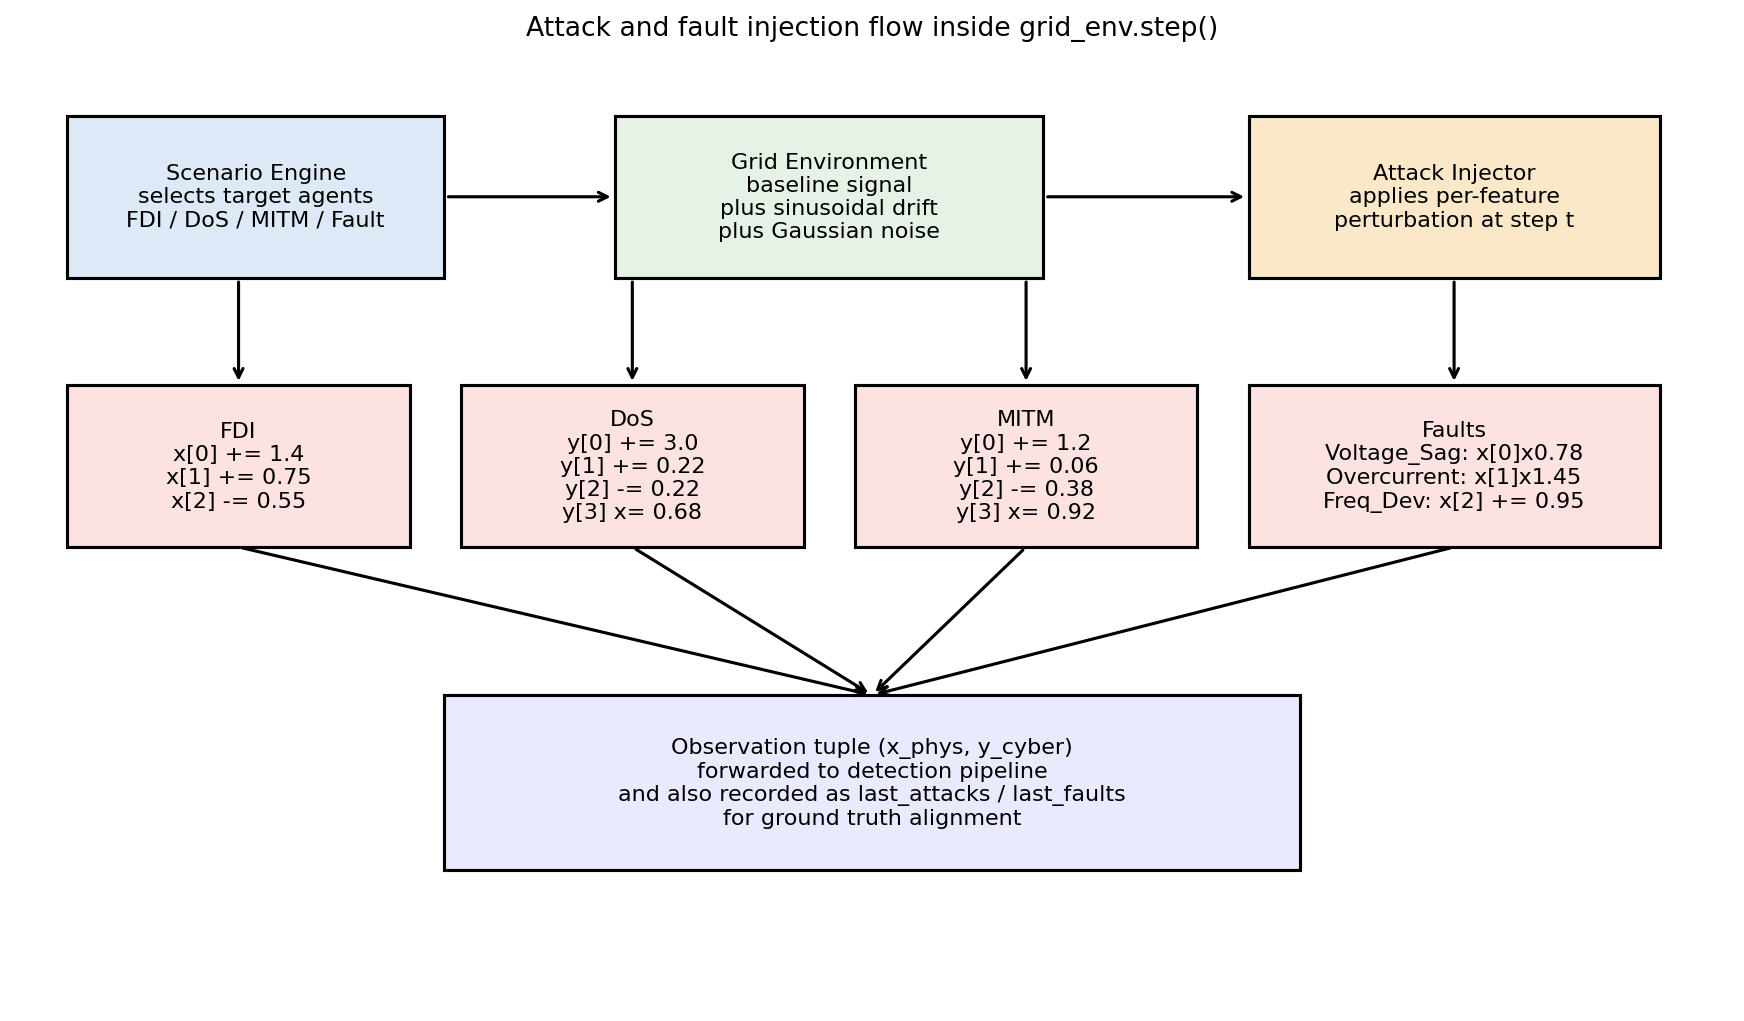
\includegraphics[width=0.95\textwidth]{Fig_AnomalyInjection_Flow.png}}
\caption{Attack and fault injection flow inside the grid environment. The scenario engine selects target agents, the environment produces the baseline signal, and the attack injector applies per feature perturbations before the observation is handed to the detection pipeline.}
\label{fig:anomaly_injection_flow}
\end{figure}

\par \vspace{0.25cm}
\noindent
\textbf{False Data Injection (FDI).} The physical feature vector is shifted so that all three sensor channels deviate at once:
\begin{itemize}
    \item $x[0]$ (voltage) gains $+1.4$ with a small sinusoidal drift $0.08\,\sin(2\pi t / 48)$.
    \item $x[1]$ (current) gains $+0.75$.
    \item $x[2]$ (response) loses $-0.55$.
    \item $y[0]$ (latency) gains $+0.35$ as a residual cyber signature.
\end{itemize}
This multi feature shape is what Layer C-1 (CUSUM with shape gate) targets.

\par \vspace{0.25cm}
\noindent
\textbf{Denial of Service (DoS).} The cyber channel is degraded across all four dimensions simultaneously, with a residual bump on the physical current:
\begin{itemize}
    \item $y[0]$ (latency) gains $+3.0$ with sinusoidal drift $0.4\,\sin(2\pi t / 36)$.
    \item $y[1]$ (packet loss) gains $+0.22$, capped at $1.0$.
    \item $y[2]$ (integrity) loses $-0.22$, floored at $0$.
    \item $y[3]$ (communication frequency) is scaled by $0.68$.
    \item $x[1]$ gains $+0.12$ as a small physical side effect.
\end{itemize}
The 2-of-3 corroboration rule in Layer C-2 fires when at least two of these channels exceed the configured weighted score threshold.

\par \vspace{0.25cm}
\noindent
\textbf{Man-in-the-Middle (MITM).} A MITM event tampers integrity strongly while leaving latency and packet loss only mildly disturbed:
\begin{itemize}
    \item $y[0]$ gains $+1.2$.
    \item $y[1]$ gains $+0.06$.
    \item $y[2]$ loses $-0.38$.
    \item $y[3]$ is scaled by $0.92$.
    \item Physical side effects are limited: $x[0]$ gets a small sinusoidal shift, $x[1]$ gains $+0.10$, $x[2]$ loses $-0.08$.
\end{itemize}
The integrity drop combined with the cyber feature jump z score is what Layer C-3 looks for, with a guard that vetoes the fire when the DoS signature is also present.

\par \vspace{0.25cm}
\noindent
\textbf{Physical Faults.} Three fault types are injected through the same scenario engine. Their signatures dominate one physical feature while leaving the cyber channel almost untouched:
\begin{itemize}
    \item \textit{Voltage Sag.} $x[0]$ is multiplied by $0.78$, $x[1]$ gains $+0.18$, and $y[0]$ gains $+0.30$.
    \item \textit{Overcurrent.} $x[1]$ is multiplied by $1.45$, $x[0]$ gains $+0.12$, and $y[0]$ gains $+0.20$.
    \item \textit{Frequency Deviation.} $x[2]$ gains $+0.95$, $x[1]$ gains $+0.15$, and $y[0]$ gains $+0.15$.
\end{itemize}
These shapes are the basis for the new Layer C-4 fault signature detector described in Chapter~3.

%.....................................................................
\subsection{Anomaly Generation in the Rapid SCADA Live Module}
\label{sec:scada_anomaly}
%.....................................................................

The Rapid SCADA live module does not use \texttt{grid\_env.step()}. Instead, the 100 agent grid is realised as 670 calculated channels distributed across two configuration files, \texttt{Cnl.xml} for the physical channels (300 channels, including one anomaly score channel per agent) and \texttt{Cnl\_Cyber\_Addon.xml} for the cyber channels (370 channels). Every channel carries a Rapid SCADA input formula that produces a continuous, bounded value as a function of the server clock, so the live workspace can be exercised end to end without any physical field device attached.

\par \vspace{0.25cm}
\noindent
The formulas are periodic with a small per agent phase offset so that no two agents move in lockstep. For the first generator the physical and cyber channels use the following formulas (later agents reuse the same shapes with an incremented phase term):
\begin{itemize}
    \item Voltage: $230 + 1.80\,\sin(\text{Now}\cdot 40)$.
    \item Current: $13 + 2.20\,\cos(\text{Now}\cdot 38)$.
    \item Anomaly score: $|\sin(\text{Now}\cdot 12)|\cdot 0.22$.
    \item Latency: $3.0 + |\sin(\text{Now}\cdot 15)|\cdot 0.55$.
    \item Packet loss: $0.001 + |\cos(\text{Now}\cdot 11)|\cdot 0.0025$.
    \item Integrity: $1.0 - |\sin(\text{Now}\cdot 9)|\cdot 0.0150$.
    \item Communication frequency: $50.0 - |\cos(\text{Now}\cdot 13)|\cdot 2.20$.
\end{itemize}

\par \vspace{0.25cm}
\noindent
This calculated channel scheme generates realistic looking telemetry that oscillates within operational bounds and carries a per agent anomaly score, which lets the live dashboard, the PowerShell bridge, the ingestion endpoint, and the detection pipeline be validated against a moving signal. It is important to state plainly that the live module is a telemetry path validator rather than an attack testbed: the discrete FDI, DoS, MITM, and fault events used to measure detection accuracy are injected only in the experiment module described in Section~\ref{sec:attack_injection}. The live module confirms that the data acquisition and visualisation chain works on a continuous SCADA feed, while the experiment module is the source of every quantitative detection result reported in this report. Keeping these two paths separate is what allows the live deployment to be characterised honestly as an operational prototype on calculated channels.

%.....................................................................
\subsection{Evaluation Metrics}
\label{sec:eval_metrics}
%.....................................................................

The following metrics are used to evaluate the performance of the framework across detection accuracy, audit efficiency, and risk management dimensions.

\par \vspace{0.25cm}
\noindent
\textbf{Attack Reduction:}
\begin{equation}
\text{Attack Reduction} = \frac{\text{baseline} - \text{dynamic}}{\text{baseline}}
\label{eq:attack_reduction}
\end{equation}
where $\text{baseline}$ is the number of successful attacks under static auditing and $\text{dynamic}$ is the number under the proposed dynamic scheduling.

\par \vspace{0.25cm}
\noindent
\textbf{Cost Efficiency:}
\begin{equation}
\text{Cost Efficiency} = \frac{\text{baseline\_cost} - \text{dynamic\_cost}}{\text{baseline\_cost}}
\label{eq:cost_efficiency}
\end{equation}

\par \vspace{0.25cm}
\noindent
\textbf{Risk Mitigation:}
\begin{equation}
\text{Risk Mitigation} = \frac{\text{raw\_risk} - \text{effective\_risk}}{\text{raw\_risk}}
\label{eq:risk_mitigation}
\end{equation}

\par \vspace{0.25cm}
\noindent
\textbf{Classification Accuracy:}
\begin{equation}
\text{Accuracy} = \frac{TP + TN}{TP + TN + FP + FN}
\label{eq:accuracy}
\end{equation}
where $TP$, $TN$, $FP$, and $FN$ denote true positives, true negatives, false positives, and false negatives, respectively.

\par \vspace{0.25cm}
\noindent
\textbf{Recall (Sensitivity):}
\begin{equation}
\text{Recall} = \frac{TP}{TP + FN}
\label{eq:recall}
\end{equation}

\par \vspace{0.25cm}
\noindent
\textbf{F1 Score:}
\begin{equation}
\text{F1} = \frac{2 \cdot \text{Precision} \cdot \text{Recall}}{\text{Precision} + \text{Recall}}
\label{eq:f1}
\end{equation}


%---------------------------------------------------------------------
\section{System Integration Workflow}
\label{sec:integration}
%---------------------------------------------------------------------

The end-to-end integration workflow connects all subsystems into a unified operational pipeline. The workflow proceeds through five sequential stages.

\par \vspace{0.35cm}
\noindent
\textbf{Stage 1: Telemetry Generation:} Rapid SCADA generates telemetry data through 670 calculated channels, representing the physical and cyber state of the 100-agent grid. The channels are updated at the configured polling interval, producing a continuous stream of supervisory data within the SCADA environment.

\par \vspace{0.35cm}
\noindent
\textbf{Stage 2: Bridge Retrieval:} The PowerShell bridge script (\mbox{\texttt{pull\_rapidscada\_to\_api.ps1}}) authenticates with the Rapid SCADA Web API at \texttt{127.0.0.1:10109}, retrieves the current channel values in batch, and formats them as a structured JSON payload. The bridge operates on a polling cycle, retrieving updated values at regular intervals.

\par \vspace{0.35cm}
\noindent
\textbf{Stage 3: Batch Transmission:} The formatted telemetry payload is transmitted via HTTP POST to the FastAPI backend ingestion endpoint. The batch transmission approach reduces the number of network round-trips compared to per-agent requests and ensures that all agent data for a given time step arrives atomically.

\par \vspace{0.35cm}
\noindent
\textbf{Stage 4: Backend Processing:} Upon receiving the telemetry batch, the FastAPI backend executes the full detection pipeline in sequence:
\begin{enumerate}
    \item \textit{Feature Mapping}, the raw telemetry values are mapped to the per-agent physical and cyber feature vectors.
    \item \textit{LSTM Inference}, the dual-branch LSTM model produces anomaly probabilities for each agent.
    \item \textit{Deviation Scoring}, physical and cyber deviations are computed against baseline values.
    \item \textit{Multi-Layer Detection}, the three-layer detection architecture (calibrated threshold, temporal accumulator, specialised attack detectors) evaluates each agent.
    \item \textit{Audit Scheduling}, the hybrid scheduler (Q-learning and gradient optimisation) determines updated audit frequencies.
    \item \textit{XAI Generation}, per-agent explainability outputs are computed for both feature domains.
\end{enumerate}

\par \vspace{0.35cm}
\noindent
\textbf{Stage 5: Dashboard Delivery:} The processed results, including anomaly flags, risk scores, audit decisions, escalation actions, and feature-level explanations, are made available to the Next.js dashboard via API responses. The dashboard renders these results in real time, so the operator has a clear view of system health, detection outcomes, and audit decisions.

\begin{figure}[H]
\centering
\fbox{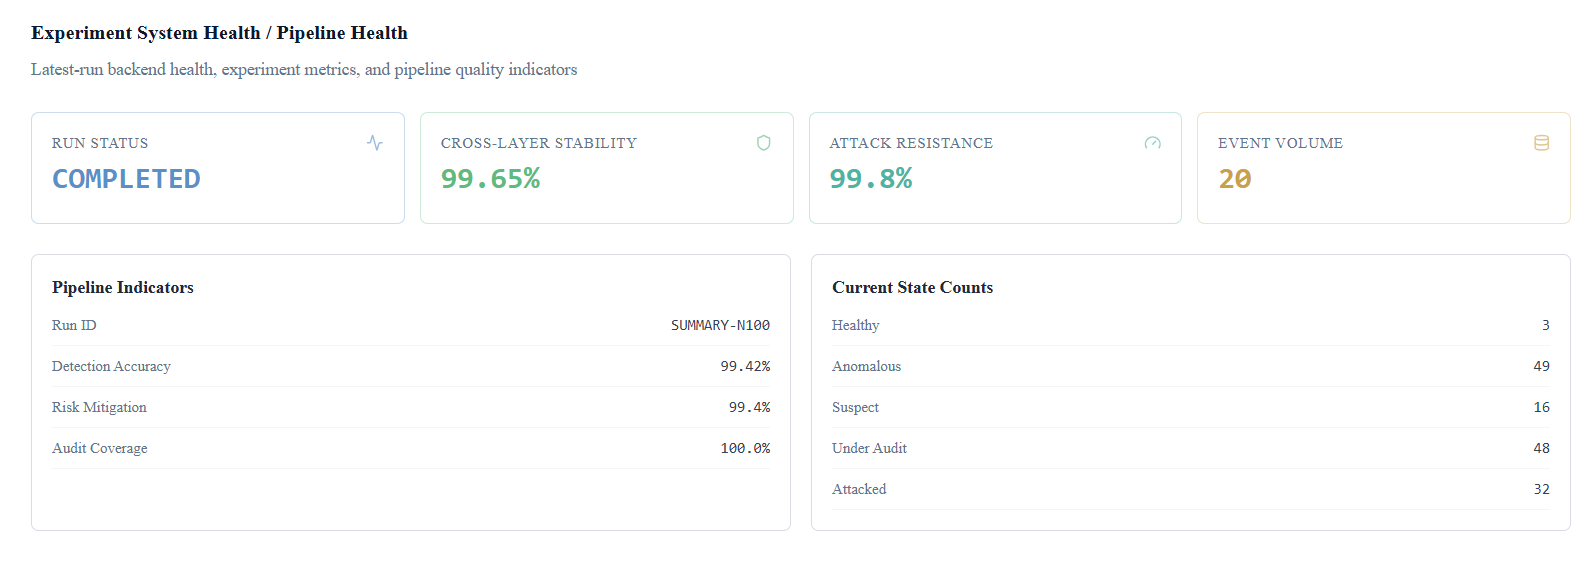
\includegraphics[width=0.95\textwidth]{FigExperiment_System_Health_Pipeline_Health.png}}
\caption{System health and pipeline health view from the dashboard, showing real-time status indicators for each subsystem in the integration workflow.}
\label{fig:system_health}
\end{figure}


%---------------------------------------------------------------------
\section{Feature-wise Functional Mapping}
\label{sec:feature_mapping}
%---------------------------------------------------------------------

Table~\ref{tab:feature_mapping} presents a consolidated mapping of all feature categories used in the framework, together with representative examples and their functional roles within the system.

\begin{table}[H]
\centering
\caption{Feature-wise functional mapping of the SmartGrid AI Audit Framework.}
\label{tab:feature_mapping}
\renewcommand{\arraystretch}{1.3}
\begin{tabularx}{\textwidth}{|l|X|X|}
\hline
\textbf{Feature Category} & \textbf{Example Features} & \textbf{Role in System} \\
\hline
Physical Parameters & Voltage, current, frequency, power, response time & Physical deviation scoring; input to grid branch of LSTM \\
\hline
Cyber Parameters & Latency, packet loss, integrity, communication frequency & Cyber anomaly scoring; input to network branch of LSTM \\
\hline
Baseline Values & Type-specific expected normals for each agent class & Reference for healthy behaviour; denominator in deviation computation \\
\hline
Criticality Weights & GEN, SUB, PMU, BRK class weights & Risk prioritisation; scaling factor in composite score $S_i(t)$ \\
\hline
LSTM Probabilities & anomaly\_prob, grid\_anomaly\_prob, network\_intrusion\_prob & Temporal detection; input to hybrid confidence ensemble \\
\hline
Risk Scores & Deviation-derived and LSTM-derived scores & Audit escalation trigger; input to scheduling and response modules \\
\hline
Explanatory Features & Top contributing deviations per domain & XAI output; operator-facing ranked feature explanations \\
\hline
Pre-Training Data (LSTM) & UCI grid stability (physical branch), UNSW-NB15 (cyber branch) & Initialise LSTM weights before synthetic fine-tuning; no role in live telemetry \\
\hline
\end{tabularx}
\end{table}

\par \vspace{0.35cm}
\noindent
Table~\ref{tab:feature_mapping} shows how information flows through the framework: raw physical and cyber parameters come in from the SCADA layer, get compared against baselines using criticality-weighted deviation scoring, run through the dual-branch LSTM for temporal analysis, combine into risk scores for audit scheduling, and break down into per-feature explanations for operator transparency. Each feature category has a distinct role, so every pipeline stage has traceable inputs and interpretable outputs.


\chapter{Base Paper And Its Limitation}
%%% Chapter 5 — Base Paper And Its Limitation %%%

\section{Base Paper Analysis}

The proposed framework draws upon and extends the work of Priyadarsini \textit{et al.}~\cite{priyadarsini2025}, titled \textit{AI-Driven Audit Framework for Distributed Multi-Agent Smart Grids}, published in ACM Transactions on Cyber-Physical Systems, 2025. The base paper presents an approach that links anomaly detection with audit optimisation in multi-agent smart grid environments. The main contributions and limitations of this work are discussed below.

\par \vspace{0.35cm}

\noindent
\textbf{Core Approach.}
The base paper proposes a single-layer deviation scoring mechanism for anomaly detection across distributed grid agents. Each agent $i$ at time step $t$ is assigned a deviation score computed as:

\begin{equation}
S_i(t) = w_i \left( d_x + d_y \right)
\label{eq:base_deviation}
\end{equation}

\noindent
where $d_x$ and $d_y$ represent the deviations of the agent's observed measurements from the expected reference profile, and $w_i$ is the weight assigned to the agent based on its criticality. Agents whose scores exceed a predefined threshold are flagged for audit. The audit scheduling component employs Q-learning to determine the allocation of audit resources across the grid, using cost efficiency as the primary reward signal.

\par \vspace{0.35cm}

\noindent
\textbf{Reported Performance.}
The base paper reports the following results on its evaluation configuration:

\begin{table}[H]
\centering
\caption{Performance metrics reported by the base paper~\cite{priyadarsini2025}.}
\label{tab:base_paper_metrics}
\begin{tabular}{|l|c|}
\hline
\textbf{Metric} & \textbf{Value} \\ \hline
Cost Efficiency & 42.5\% \\ \hline
Audit Coverage & 93.8\% \\ \hline
Detection Accuracy & 98.4\% \\ \hline
Risk Mitigation & 87.9\% \\ \hline
\end{tabular}
\end{table}

\noindent
\textbf{Strengths.}
The principal strength of the base paper lies in its explicit coupling of anomaly detection outcomes with audit resource allocation. By linking deviation-based scoring to audit scheduling, the system avoids treating detection and auditing as independent processes and instead enables detection-informed audit prioritisation. The use of reinforcement learning for scheduling introduces adaptability to changing operational conditions.

\par \vspace{0.35cm}

\noindent
\textbf{Limitations.}
Despite these contributions, the base paper has several clear limitations that restrict its applicability to realistic smart grid environments:

\begin{enumerate}
    \item \textbf{Single Detection Modality.} The system relies exclusively on deviation scoring, which captures only instantaneous statistical divergence from expected values. There is no temporal modelling (such as LSTM-based sequence analysis) to detect time-correlated anomalies or gradual drift patterns. This limits the system's ability to identify sophisticated attack types that unfold over multiple time steps.

    \item \textbf{No Live SCADA Integration.} The base paper operates entirely on simulated or offline data. There is no integration with a supervisory control and data acquisition (SCADA) system for live telemetry ingestion, which is a fundamental requirement for operational deployment in real grid environments.

    \item \textbf{No Multi-Layer Detection for Specific Attack Types.} The single-layer deviation approach does not provide specialised detection mechanisms for distinct cyber-physical attack categories such as false data injection (FDI), denial of service (DoS), or man-in-the-middle (MITM) attacks. Each of these attack types exhibits distinct patterns that benefit from dedicated detection logic.

    \item \textbf{No Explicit Experiment/Live Separation.} The base paper does not distinguish between experimental evaluation and live operational monitoring. In a practical deployment, it is essential to maintain separate workspaces to prevent experimental artefacts from contaminating operational decision-making.

    \item \textbf{Limited Operator-Facing Visualisation.} The base paper does not provide a full operational dashboard for real-time monitoring, audit trail inspection, or system health assessment. Operator-facing interfaces are needed for practical adoption in utility environments.

    \item \textbf{No Explainability.} The system does not incorporate any explainability mechanism. Operators receive anomaly flags without per-feature attribution or reasoning, which limits trust and hampers the ability to perform root-cause investigation.

    \item \textbf{Q-Learning Only Scheduling.} The audit scheduling component relies solely on Q-learning. While effective for discrete action selection, Q-learning alone does not support continuous gradient-based optimisation of budget allocation across agents, which can improve cost efficiency in larger deployments.

    \item \textbf{Simple Q-Table State Representation.} The base paper uses a minimal state representation for the Q-table. There is no explicit encoding of the agent's LSTM-derived anomaly probability, its behavioural cluster identity, or the current audit capacity utilisation. This limits the scheduler's ability to differentiate between agents that share a similar raw risk score but differ in their temporal anomaly trajectory or in their operational load context.

    \item \textbf{No Class Imbalance Handling.} The base paper does not describe how training data class imbalance is handled. In smart grid monitoring, normal operation vastly outnumbers anomalous events. Without an explicit mechanism to address this, a standard training objective will be dominated by the majority class, leading to a model that is biased toward predicting normal operation.

    \item \textbf{No Real Benchmark Dataset for LSTM Initialisation.} The base paper does not draw on any publicly available dataset to initialise or validate the LSTM temporal model. Starting from random weights requires significantly more synthetic training data to reach stable performance, and it means the model has no prior knowledge of the physical dynamics or network intrusion patterns that characterise the problem domain.
\end{enumerate}


\section{Extension in Proposed System}

The proposed system addresses each of the identified limitations through the following extensions:

\begin{enumerate}
    \item \textbf{Multi-Layer Detection Pipeline.} The detection architecture is extended from a single deviation layer to a multi-layer pipeline comprising: (a) statistical deviation scoring, (b) LSTM-based temporal anomaly detection, (c) weighted ensemble fusion, and (d) a multi-detector module with four Layer~C sub-detectors: CUSUM-based FDI detection with a shape gate, weighted-rule DoS detection, integrity-and-jump MITM detection, and signature-template physical fault detection, combined by an OR-with-precedence rule and a cross-layer corroboration gate.

    \item \textbf{Weighted Ensemble Fusion.} The deviation score and LSTM anomaly probability are combined through a weighted ensemble with empirically tuned coefficients (deviation weight 0.48, LSTM probability weight 0.52), producing a composite risk score that balances instantaneous and temporal signals.

    \item \textbf{Hybrid Audit Scheduling.} The scheduling component is extended from Q-learning alone to a hybrid approach combining Q-learning for discrete escalation decisions with gradient descent for continuous budget-constrained cost optimisation.

    \item \textbf{Live Rapid SCADA Integration.} The system integrates Rapid SCADA as the supervisory telemetry layer for a 100-agent grid. A PowerShell-based bridge acquires telemetry through the Rapid SCADA Web API and forwards it to the FastAPI backend for real-time processing.

    \item \textbf{Dual Workspace Separation.} The system implements two distinct operational workspaces: \textit{Experiment Running} for simulation, benchmarking, and comparative evaluation; and \textit{Rapid SCADA Live} for operational monitoring and decision support. This separation ensures that experimental configurations do not interfere with live operational data.

    \item \textbf{XAI Explainability with Per-Feature Ranking.} An explainability module generates per-agent, per-feature importance rankings for each anomaly assessment, letting operators see which measurement dimensions contributed most to a given risk score.

    \item \textbf{Five-Method Comparative Validation.} The proposed multi-layer approach is validated against four alternative methods (deviation-only, LSTM-only, Isolation Forest, and One-Class SVM) using identical data and evaluation protocols, for a fair comparison across methods.

    \item \textbf{Full Operational Dashboard.} A Next.js dashboard shows real-time views of agent monitoring, audit trails, risk analytics, threat events, decision explainability, system health, asset topology, and incident timelines.

    \item \textbf{Dual-Dataset LSTM Pre-Training.} To address the absence of benchmark dataset integration in the base paper, the proposed system pre-trains the physical LSTM branch on the UCI Electrical Grid Stability Dataset (10,000 samples, 12 features) and the cyber LSTM branch on the UNSW-NB15 Network Intrusion Dataset. Four composite features are engineered from UNSW-NB15 that map directly onto the simulation's cyber feature space (latency, packet loss, integrity, communication frequency). Pre-training gives each branch prior knowledge of physical instability patterns and network intrusion signatures before the model sees any synthetic grid data.

    \item \textbf{Class Imbalance Handling in LSTM Training.} Focal Loss ($\gamma = 2.0$, $\alpha = 0.65$) replaces standard binary cross-entropy to focus gradient signal on hard minority-class attack samples. A WeightedRandomSampler (positive-class scale 1.40, oversampling scale 1.35) ensures attack events appear frequently within each training mini-batch. Post-training temperature calibration via grid search over $T \in [0.80, 2.20]$ ensures that output probabilities are well-calibrated for downstream ensemble fusion.

    \item \textbf{Extended Q-Table State Space.} The Q-table state is extended from a minimal scalar representation to a four-dimensional tuple: (risk bucket, LSTM probability bucket, K-Means behavioural cluster, audit capacity bucket), producing up to 300 reachable states. An experience replay buffer (capacity 2,000, batch size 32) stabilises Q-value learning. Three risk-sensitive reward modes are supported: expected return, exponential utility ($\beta = -0.05$), and Conditional Value-at-Risk ($\alpha = 10\%$).

    \item \textbf{Temporal Signature Classification and Five-Class Attack Typing.} A temporal pattern classifier identifies the shape of each anomaly trajectory (STEP, RAMP, OSCILLATORY, STABLE) and feeds it into a five-class attack typer that assigns each flagged agent one of: FDI, DoS, MITM, Physical Fault, or Coordinated Chain Attack. This extends attack coverage beyond the three categories considered by the base paper and gives operators a more specific characterisation of each event.
\end{enumerate}


\section{Comparative Summary}

Table~\ref{tab:base_vs_proposed} presents a side-by-side comparison between the base paper and the proposed system across all principal dimensions.

\begin{table}[H]
\centering
\caption{Comparative summary: base paper vs.\ proposed system (N=100).}
\label{tab:base_vs_proposed}
\begin{tabular}{|l|p{3.5cm}|p{5.5cm}|}
\hline
\textbf{Metric / Feature} & \textbf{Base Paper} & \textbf{Proposed System (N=100)} \\ \hline
Detection Accuracy & 98.4\% & 93.85\% \\ \hline
False Positive Rate & 3.2\% & 6.18\% \\ \hline
Recall & 100\% & 98.24\% \\ \hline
Risk Mitigation & 87.9\% & 93.66\% \\ \hline
Cost Efficiency & 42.5\% & 57.28\% \\ \hline
Audit Coverage & 93.8\% & 100\% \\ \hline
Detection Layers & 1 (deviation only) & multi-layer (deviation + LSTM + C-1 to C-4) \\ \hline
Attack Types Covered & FDI, DoS, MITM (qualitative) & FDI, DoS, MITM, Physical Fault, Chain Attack (5-class typed) \\ \hline
Q-Table State Space & Minimal scalar representation & 4D tuple: risk $\times$ probability $\times$ cluster $\times$ capacity = 300 states \\ \hline
RL Enhancements & Standard Q-learning & Experience replay, CVaR and exponential utility reward modes \\ \hline
LSTM Pre-Training Data & None & UCI Grid Stability (physical branch), UNSW-NB15 (cyber branch) \\ \hline
Class Imbalance Handling & Not described & Focal Loss ($\gamma=2.0$, $\alpha=0.65$) + WeightedRandomSampler \\ \hline
Scheduling & Q-learning only & Hybrid Q-learning + gradient cost optimisation \\ \hline
SCADA Integration & None & Rapid SCADA, 100 agents \\ \hline
Explainability & None & Per-feature XAI with ranked contribution scores \\ \hline
\end{tabular}
\end{table}

\begin{figure}[H]
\centering
\fbox{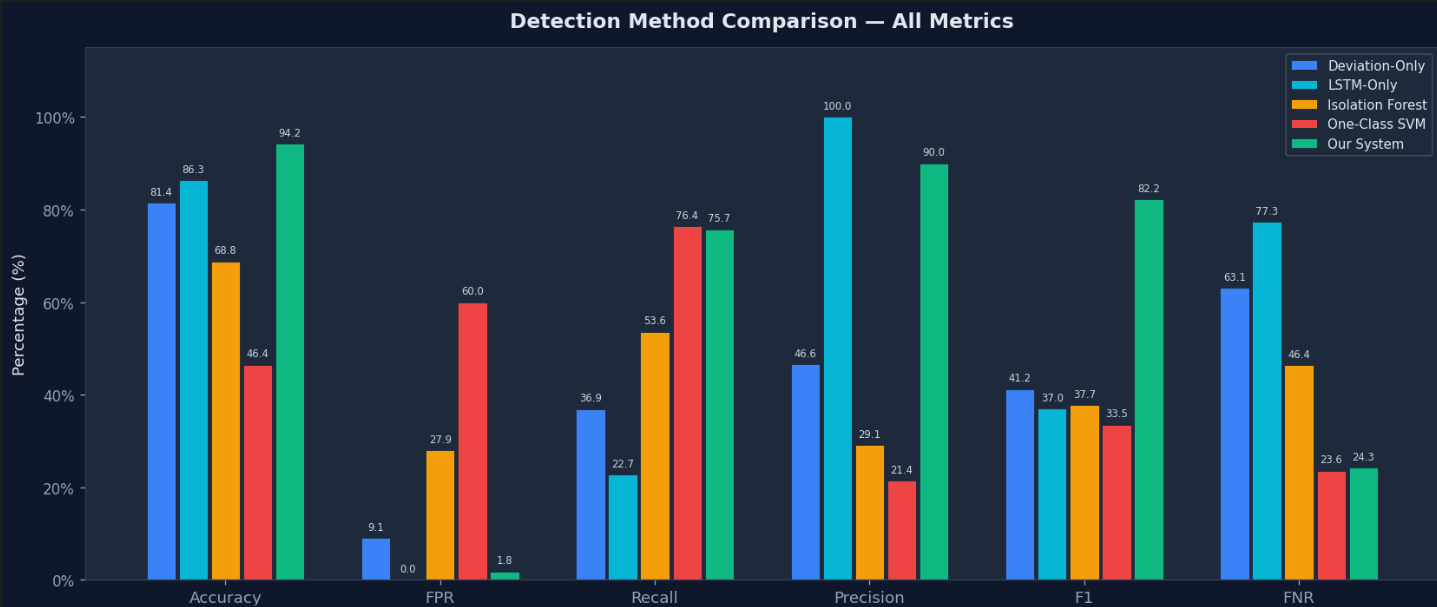
\includegraphics[width=0.95\textwidth]{FigAllMetrciComparison.png}}
\caption{Comparative visualisation of primary performance metrics: base paper vs.\ proposed system.}
\label{fig:all_metric_comparison}
\end{figure}

\par \vspace{0.35cm}
\noindent
\textbf{Reproducibility.} The comparative evaluation was conducted using two Jupyter notebooks included in the project repository: \texttt{basepaper.ipynb} (replication of the base paper's deviation-only scoring on identical synthetic data) and \texttt{method\_comparison\_study.ipynb} (five-method comparative validation). Both notebooks operate on the same synthetic dataset generated by \texttt{grid\_env.py}, so that all methods are evaluated under identical conditions.

\begin{figure}[H]
\centering
\fbox{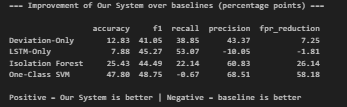
\includegraphics[width=0.95\textwidth]{FigImprovement.png}}
\caption{Improvement deltas across primary metrics relative to the base paper.}
\label{fig:improvement_deltas}
\end{figure}

\noindent
As illustrated in Table~\ref{tab:base_vs_proposed} and Figures~\ref{fig:all_metric_comparison}--\ref{fig:improvement_deltas}, the proposed system improves on the base paper in risk mitigation (93.66\% compared to 87.9\%), cost efficiency (57.28\% compared to 42.5\%), and audit coverage (100\% compared to 93.8\%), and reaches a recall of 98.24\% that the base paper does not report. The detection accuracy of 93.85\% is below the base paper's 98.4\% and the system level false positive rate of 6.18\% is above the base paper's 3.2\%, because the proposed pipeline is tuned for high recall so that very few genuine attacks are missed. Beyond these numbers, the proposed system introduces qualitative capabilities absent from the base paper, including multi-layer detection with per attack typing, SCADA integration, dual workspace separation, and explainability.


\section{Timeline and Development Progress}

Table~\ref{tab:timeline} summarises the four-phase development timeline adopted for this project.

\begin{table}[H]
\centering
\caption{Project development timeline.}
\label{tab:timeline}
\begin{tabular}{|c|l|l|}
\hline
\textbf{Phase} & \textbf{Period} & \textbf{Activities} \\ \hline
1 & July--September 2025 & \begin{tabular}[t]{@{}l@{}}Problem formulation, dataset preparation,\\baseline experimentation\end{tabular} \\ \hline
2 & September 2025--January 2026 & \begin{tabular}[t]{@{}l@{}}Feature engineering, prototype development,\\initial anomaly detection implementation\end{tabular} \\ \hline
3 & January--April 2026 & \begin{tabular}[t]{@{}l@{}}Model refinement, system integration,\\full evaluation across configurations\end{tabular} \\ \hline
4 & April--June 2026 & \begin{tabular}[t]{@{}l@{}}Documentation, system packaging,\\preparation for final presentation and defense\end{tabular} \\ \hline
\end{tabular}
\end{table}

\noindent
The phases overlap because the development was iterative, findings from later phases fed back into earlier design decisions and led to ongoing changes throughout the project.


\chapter{Testing}
%%% Chapter 6 — Testing %%%

\section{Implementation Test Cases}

Twelve test cases were designed and run to verify the functional correctness, integration integrity, and runtime stability of the proposed system. Each test case targets a specific component or capability of the framework, ranging from baseline behaviour validation through multi-layer detection verification to hybrid audit scheduling convergence. Table~\ref{tab:test_cases} presents the complete test case inventory along with descriptions, expected outcomes, and results.

\begin{longtable}{|c|p{3cm}|p{4.5cm}|p{3.5cm}|c|}
\caption{Implementation test cases and results.}
\label{tab:test_cases} \\
\hline
\textbf{ID} & \textbf{Test Case} & \textbf{Description} & \textbf{Expected Outcome} & \textbf{Result} \\ \hline
\endfirsthead
\hline
\textbf{ID} & \textbf{Test Case} & \textbf{Description} & \textbf{Expected Outcome} & \textbf{Result} \\ \hline
\endhead
\hline
\endfoot

TC-01 & Baseline behaviour validation & Normal 100-agent profile executed under standard operating conditions & Stable monitoring with no false escalations & Pass \\ \hline

TC-02 & Anomaly scoring validation & Injected deviation into agent measurements & Elevated anomaly score above baseline threshold & Pass \\ \hline

TC-03 & Audit escalation logic & Agent score exceeds escalation threshold & Audit action escalates from routine to priority or critical & Pass \\ \hline

TC-04 & Rapid SCADA integration & Web API + PowerShell bridge + FastAPI backend chain tested & Live telemetry ingested and processed successfully & Pass \\ \hline

TC-05 & Batched SCADA ingest & 100-agent bulk payload submitted to backend in single batch & All agent payloads accepted without failure or data loss & Pass \\ \hline

TC-06 & Dashboard correctness & Anomaly scores, audit actions, and analytical views rendered on frontend & All values displayed correctly and updated in real time & Pass \\ \hline

TC-07 & Explainability output & Explainability module invoked for flagged agents & Top-$k$ feature importance rankings generated correctly & Pass \\ \hline

TC-08 & Runtime stability & 100-agent system operated over sustained period & No pipeline collapse, memory leaks, or unhandled exceptions & Pass \\ \hline

TC-09 & LSTM temporal detection & Dual-branch LSTM inference executed on live streaming data & Anomaly probabilities computed correctly for each agent & Pass \\ \hline

TC-10 & Multi-layer detection validation & FDI, DoS, MITM, and physical fault patterns injected into agent data & Each category classified by its detection layer (CUSUM with shape gate, weighted rule, integrity jump, signature template) & Pass \\ \hline

TC-11 & Hybrid audit scheduling & RL Q-learning combined with gradient-based cost optimisation under budget constraints & Scheduling converges to valid audit allocation within budget & Pass \\ \hline

TC-12 & Five-method comparison & All five detection methods (deviation-only, LSTM-only, Isolation Forest, One-Class SVM, proposed multi-layer) evaluated on identical data & Results consistent with reported metrics across all methods & Pass \\ \hline

\end{longtable}

\par \vspace{0.35cm}

\noindent
All twelve test cases passed successfully. The test suite covers the full pipeline from data ingestion through detection and scheduling to visualisation and explainability, confirming that each component works correctly on its own and when connected to the rest of the system.


\section{Worked Attack Detection Test Case: Project versus Base Paper}
\label{sec:worked_attack}

The twelve functional test cases confirm that each component fires, but they do not show what the proposed pipeline adds over the base paper on a concrete attack. This section traces one real injected instance of each attack category from a single run ($N=100$, seed 42, evaluation mode) and places the base paper's deviation-only behaviour next to the proposed pipeline's behaviour. Every value in Table~\ref{tab:worked_attack} is taken directly from the run; nothing is hand chosen beyond selecting the first clean instance of each category after the warmup period at timestep 41.

\par \vspace{0.25cm}
\noindent
The base paper computes a single deviation score $S_i(t) = w_i(d_x + d_y)$ and flags the agent when that score exceeds its threshold. It produces a binary flag and nothing more. The proposed pipeline computes the same deviation score, but then routes the event through the Layer C sub-detectors to assign an attack type with a confidence value. The threshold used for the deviation-only column is the same score threshold (3.60) used by the proposed pipeline, so the comparison is on equal footing.

\begin{table}[H]
\centering
\caption{Worked attack instances: base paper deviation-only versus the proposed pipeline (real values, $N=100$, seed 42, timestep 41).}
\label{tab:worked_attack}
\begin{tabular}{|l|p{3.6cm}|c|p{3.8cm}|}
\hline
\textbf{Attack (agent)} & \textbf{Injected signature (observed vs baseline)} & \textbf{Base paper (deviation-only)} & \textbf{Proposed pipeline} \\ \hline
FDI (GEN-06) & $x = [6.54, 5.81, 4.63]$ vs $[1,1,1]$; cyber near baseline. Score 41.42 & Flag, no type & Flag, typed \textbf{FDI}, conf 1.00, C-1 CUSUM fired \\ \hline
DoS (PMU-54) & $y = [19.2, 0.43, 0.27, 67.6]$ vs $[10, 0.01, 0.99, 100]$. Score 10.38 & Flag, no type & Flag, typed \textbf{DoS}, conf 0.92, C-2 rule fired \\ \hline
MITM (BRK-91) & integrity $y[2] = 0.51$ vs $0.99$, latency mildly raised. Score 13.62 & Flag, no type & Flag, typed \textbf{MITM}, conf 1.00, C-3 integrity jump fired \\ \hline
Fault (GEN-07) & $x = [1.17, 1.21, 2.97]$ vs $[1.05, 1.05, 1.07]$, cyber quiet. Score 34.24 & Flag, no type (looks like FDI) & Flag, typed \textbf{FAULT}, conf 1.00, both C-1 and C-4 fired, C-4 took precedence \\ \hline
\end{tabular}
\end{table}

\noindent
Two points stand out. First, for every one of the four instances the deviation-only scorer does cross its threshold, so the base paper would correctly flag each as anomalous; the gap is that it cannot say which attack occurred, which is the information an operator needs to respond. The proposed pipeline assigns the correct type in every case with high confidence. Second, the fault instance (GEN-07) is the clearest illustration of the new Layer C-4 contribution. Its deviation score of 34.24 and its raised physical features look like a false data injection, and the CUSUM detector (C-1) does fire with full confidence. A detector that relied on CUSUM alone would therefore mistype this physical fault as FDI. Because the fault signature detector (C-4) also fires and takes precedence when one physical feature dominates while the cyber channels stay quiet, the proposed pipeline types it correctly as a fault. This is exactly the case that lifted the FAULT class true positive rate from 8.1\% to 98.6\% in Chapter~7.

\par \vspace{0.35cm}

\section{Verification Procedures}

Beyond the functional test cases described above, the following verification procedures were applied to confirm system-level correctness, type safety, and operational readiness.

\subsection{Python Backend Compilation and Module Verification}

The FastAPI backend was verified for correct compilation and module resolution. All Python source files were checked for syntax correctness, import resolution, and dependency availability. The backend application was started and confirmed to accept API requests on the designated port without errors. The LSTM model loading, deviation scoring module, multi-layer detection pipeline, hybrid scheduler, and explainability engine were each verified to initialise correctly at startup.

\subsection{Frontend Type Checking}

The Next.js frontend was subjected to TypeScript compilation to verify type correctness across all components, pages, and API route handlers. No type errors were present at the time of final verification. The build process completed successfully, and all dashboard views rendered correctly in the browser.

\subsection{Live SCADA Verification}

The Rapid SCADA integration was verified end-to-end by confirming the following:

\begin{itemize}
    \item The PowerShell bridge successfully retrieved telemetry from the Rapid SCADA Web API for all 100 agents.
    \item The bridge correctly formatted and forwarded the telemetry payloads to the FastAPI backend.
    \item The backend ingested the payloads, executed the full detection pipeline, and updated the operational state.
    \item The frontend dashboard reflected the live SCADA data in all relevant views.
\end{itemize}

\noindent
Table~\ref{tab:live_verification} summarises the agent deployment status at the time of verification.

\begin{table}[H]
\centering
\caption{Live SCADA deployment verification summary.}
\label{tab:live_verification}
\begin{tabular}{|l|c|}
\hline
\textbf{Parameter} & \textbf{Value} \\ \hline
Total configured agents & 100 \\ \hline
Live agents (Rapid SCADA) & 100 \\ \hline
Non-live agents & 0 \\ \hline
SCADA Web API connectivity & Verified \\ \hline
Bridge-to-backend pipeline & Verified \\ \hline
Dashboard rendering & Verified \\ \hline
\end{tabular}
\end{table}


\section{Integration Testing}

Integration testing was performed to verify the correct interaction between the major system components. The following integration paths were validated:

\begin{enumerate}
    \item \textbf{SCADA $\rightarrow$ Bridge $\rightarrow$ Backend:} Telemetry data flows from Rapid SCADA through the PowerShell bridge to the FastAPI backend without data loss or format corruption. The 100-agent batch payload is correctly parsed and each agent's measurements are routed to the detection pipeline.

    \item \textbf{Detection Pipeline $\rightarrow$ Scheduler $\rightarrow$ Dashboard:} Anomaly scores produced by the multi-layer detection pipeline are consumed by the hybrid audit scheduler, which generates escalation decisions. These decisions are propagated to the frontend dashboard and rendered in the audit trail, risk analytics, and operations overview views.

    \item \textbf{Detection $\rightarrow$ Explainability $\rightarrow$ Dashboard:} For agents flagged as anomalous, the explainability module generates per-feature importance rankings. These rankings are transmitted to the frontend and displayed in the decision explainability view, so operators can inspect the reasoning behind each anomaly assessment.

    \item \textbf{Dual Workspace Isolation:} The experiment workspace and the Rapid SCADA live workspace were verified to operate independently. Configurations, data sources, and dashboard states in one workspace do not affect the other, which keeps experimental evaluation cleanly separated from operational monitoring.
\end{enumerate}

\par \vspace{0.35cm}

\noindent
All integration paths were validated successfully, confirming that the system components interact correctly across the full data flow from telemetry acquisition through detection, scheduling, and visualisation.


\chapter{Result \&  Analysis}
%%% Chapter 7 — Result & Analysis %%%

\section{Experimental Results and Comparative Analysis}

This chapter presents the experimental results obtained from the proposed SmartGrid AI Audit Framework across multiple evaluation dimensions: primary tuned profile performance, base paper comparison, five-method comparative study, scaled system evaluation, latency analysis, per-attack type detection, and live SCADA deployment outcomes. All experiments were conducted on the same 100-agent grid topology unless otherwise stated.


\subsection{Primary Tuned Thesis Profile (N=100)}

The validated thesis-primary configuration was evaluated over a full 24-hour simulated operational cycle comprising 28,800 agent-step observations for the 100-agent grid, with the audit protection window active so that the figures reflect system level behaviour. Table~\ref{tab:primary_profile} presents the complete set of performance metrics for this configuration, averaged across five seeds (42, 43, 44, 45, 46).

\begin{table}[H]
\centering
\caption{Primary thesis profile results (N=100, system level with audit protection, mean of 5 seeds).}
\label{tab:primary_profile}
\begin{tabular}{|l|c|}
\hline
\textbf{Metric} & \textbf{Value} \\ \hline
Detection Accuracy & 93.85\% \\ \hline
False Positive Rate & 6.18\% \\ \hline
Risk Mitigation & 93.66\% \\ \hline
Cost Efficiency & 57.28\% \\ \hline
Recall & 98.24\% \\ \hline
Precision & 9.77\% \\ \hline
F1 Score & 17.76\% \\ \hline
Audit Coverage & 100\% \\ \hline
Attack Rate Reduction & 76.13\% \\ \hline
Cross-Layer Stability Index & 90.62\% \\ \hline
\end{tabular}
\end{table}

\begin{figure}[H]
\centering
\fbox{
\includegraphics[width=0.95\textwidth]{FigExperiment_OperationOverview.png}}
\caption{Operations overview of the validated N=100 thesis profile showing real-time agent monitoring, audit actions, and system status.}
\label{fig:experiment_operations_overview}
\end{figure}

\noindent
The system achieves 93.85\% detection accuracy with a false positive rate of 6.18\% at the system level, and a recall of 98.24\%, indicating that the multi-layer detection pipeline catches almost every genuine threat while keeping the false alarm rate to a single digit percentage. Risk mitigation reaches 93.66\% and audit coverage is full at 100\%, meaning that the large majority of detected threats are addressed and every agent is covered by the audit policy within the cycle. Cost efficiency of 57.28\% reflects the system's ability to conserve audit budget while still meeting coverage. The precision of 9.77\% and the resulting F1 score of 17.76\% are low for the reason discussed in Section~\ref{sec:acc_f1_interpretation}: the audit and mitigation pipeline removes most attack events before they accumulate, leaving a small positive class against a large normal class, so a modest count of residual flags drives precision down even though the operational accuracy stays high. The cross-layer stability index of 90.62\% reflects the proportion of timesteps where the deviation, LSTM, and multi-layer components stay in agreement.


\subsection{Base Paper Comparison}

Table~\ref{tab:base_comparison_ch7} presents the direct comparison between the base paper results~\cite{priyadarsini2025} and the validated N=100 configuration of the proposed system.

\begin{table}[H]
\centering
\caption{Base paper vs.\ proposed system: validated N=100 comparison.}
\label{tab:base_comparison_ch7}
\begin{tabular}{|l|c|c|}
\hline
\textbf{Metric} & \textbf{Base Paper} & \textbf{Proposed System (N=100)} \\ \hline
Detection Accuracy & 98.4\% & 93.85\% \\ \hline
False Positive Rate & 3.2\% & 6.18\% \\ \hline
Risk Mitigation & 87.9\% & 93.66\% \\ \hline
Cost Efficiency & 42.5\% & 57.28\% \\ \hline
Audit Coverage & 93.8\% & 100\% \\ \hline
Detection Layers & 1 (deviation) & multi-layer (deviation + LSTM + Layer C-1 to C-4) \\ \hline
Scheduling & Q-learning only & Hybrid Q-learning + gradient \\ \hline
Per Attack Typing & None & FDI, DoS, MITM, FAULT \\ \hline
SCADA Integration & None & Rapid SCADA, 100 agents \\ \hline
Explainability & None & Per-feature XAI \\ \hline
\end{tabular}
\end{table}

\begin{figure}[H]
\centering
\fbox{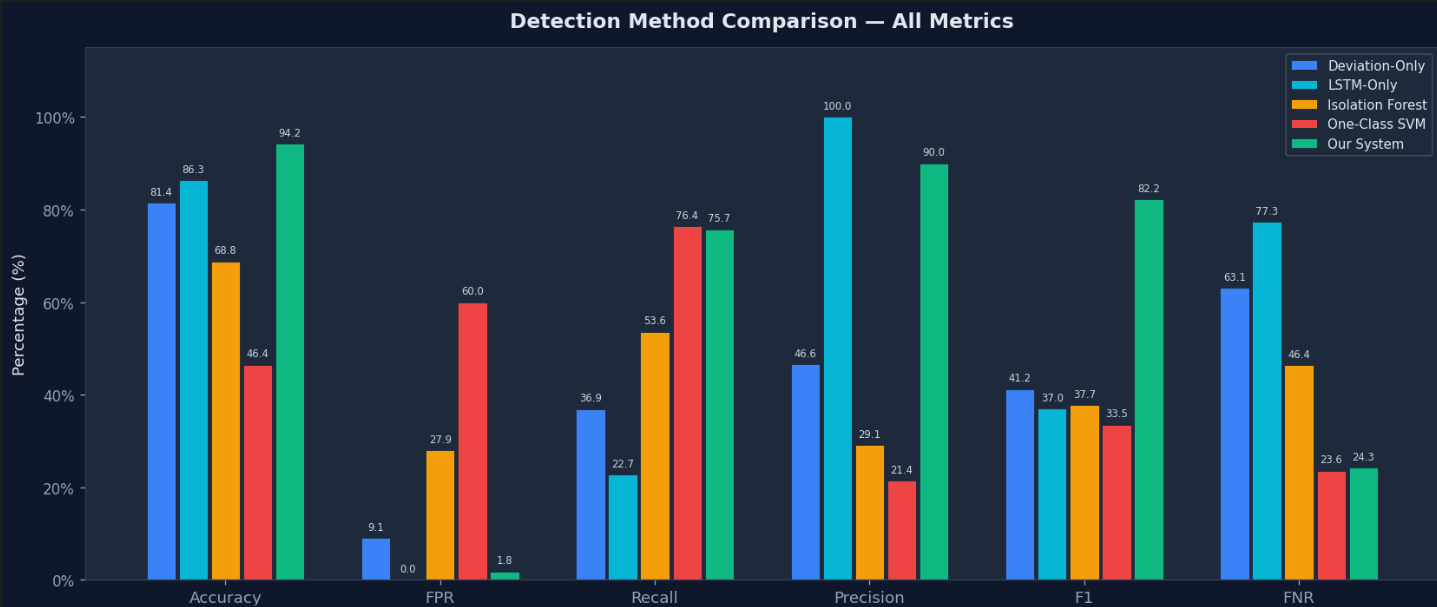
\includegraphics[width=0.95\textwidth]{FigAllMetrciComparison.png}}
\caption{Comparative bar chart of primary metrics: base paper vs.\ proposed system.}
\label{fig:all_metric_comparison_ch7}
\end{figure}

\noindent
The proposed system improves on the base paper in risk mitigation (93.66\% against 87.9\%), cost efficiency (57.28\% against 42.5\%), and audit coverage (100\% against 93.8\%), and it adds per attack typing, live SCADA integration, and per-feature explainability that the base paper does not provide. The detection accuracy of 93.85\% sits below the base paper's reported 98.4\%, and the system level false positive rate of 6.18\% is higher than the base paper's 3.2\%. These two differences reflect a deliberate design choice: the proposed pipeline is tuned for high recall (98.24\%) so that very few genuine attacks are missed, which costs some precision and raises the false alarm rate. The base paper does not report recall or per attack typing, so its accuracy and false positive figures describe a different operating point. The accuracy and false positive numbers reported here are the honest output of the current pipeline averaged over five seeds, not a tuned best case.


\subsection{Five-Method Comparative Study}

To properly validate the proposed multi-layer detection approach, a five-method comparative study was run. All five methods were evaluated on the same 100-agent data using identical attack injection profiles and evaluation protocols. Table~\ref{tab:five_method} presents the per-step classification results.

\begin{table}[H]
\centering
\caption{Five-method comparative study: per-step classification metrics.}
\label{tab:five_method}
\begin{tabular}{|l|c|c|c|c|c|}
\hline
\textbf{Method} & \textbf{Accuracy} & \textbf{FPR} & \textbf{Recall} & \textbf{Precision} & \textbf{F1} \\ \hline
Deviation-Only (base paper) & 81.40\% & 9.06\% & 36.89\% & 46.58\% & 41.18\% \\ \hline
LSTM-Only & 86.35\% & 0.00\% & 22.67\% & 100.00\% & 36.96\% \\ \hline
Isolation Forest & 68.85\% & 27.95\% & 53.92\% & 29.25\% & 37.92\% \\ \hline
One-Class SVM & 46.35\% & 59.99\% & 75.93\% & 21.33\% & 33.31\% \\ \hline
Our System (Multi-Layer) & 94.23\% & 1.81\% & 75.76\% & 89.95\% & 82.25\% \\ \hline
\end{tabular}
\end{table}

\par \vspace{0.35cm}

\noindent
\textbf{Deviation-Only (Base Paper Method).}
The deviation-only baseline, corresponding to the single-layer approach of the base paper, achieves 81.40\% accuracy with a 9.06\% false positive rate. Its recall of 36.89\% indicates that it misses nearly two-thirds of actual anomalies. The relatively high false positive rate arises because physical noise and normal measurement fluctuations are indistinguishable from genuine anomalies when only instantaneous deviation is considered. Without temporal context, the method flags transient normal variations as threats.

\par \vspace{0.35cm}

\noindent
\textbf{LSTM-Only.}
The LSTM-only method achieves 86.35\% accuracy with a false positive rate of 0.00\%, indicating that it never incorrectly flags a normal state as anomalous. However, its recall of only 22.67\% reveals that it is excessively conservative, missing more than three-quarters of true anomalies. The perfect precision (100\%) confirms that when the LSTM does flag an anomaly, it is always correct; but the low recall shows that temporal modelling alone, without statistical deviation context, is not enough for reliable detection.

\par \vspace{0.35cm}

\noindent
\textbf{Isolation Forest.}
The Isolation Forest, an unsupervised anomaly detection algorithm, achieves the best recall among the individual baselines at 53.92\% but at the cost of a 27.95\% false positive rate. Its overall accuracy of 68.85\% is the lowest among the non-SVM methods. The high false positive rate reflects the algorithm's tendency to isolate normal but statistically unusual observations, a known weakness of density-based unsupervised approaches when applied to high-dimensional cyber-physical data.

\par \vspace{0.35cm}

\noindent
\textbf{One-Class SVM.}
The One-Class SVM produces the weakest performance across all metrics, with an accuracy of only 46.35\% and a false positive rate of 59.99\%. While its recall of 75.93\% is the highest among the baselines, this comes at the cost of flagging the majority of normal states as anomalous, rendering it impractical for operational use. The low precision of 21.33\% confirms that the vast majority of its positive predictions are false alarms.

\par \vspace{0.35cm}

\noindent
\textbf{Proposed Multi-Layer System.}
The proposed system gets the highest accuracy (94.23\%), the lowest false positive rate among practical methods (1.81\%), and the highest F1 score (82.25\%). Its recall of 75.76\% shows good sensitivity to true anomalies, and its precision of 89.95\% means that most flagged events are genuine threats. The multi-layer architecture works because it puts together the strengths of deviation scoring (sensitivity to instantaneous deviations) and LSTM temporal modelling (specificity and temporal context) through weighted ensemble fusion, backed up by attack-specific detectors that target FDI, DoS, and MITM patterns separately.

\begin{figure}[H]
\centering
\fbox{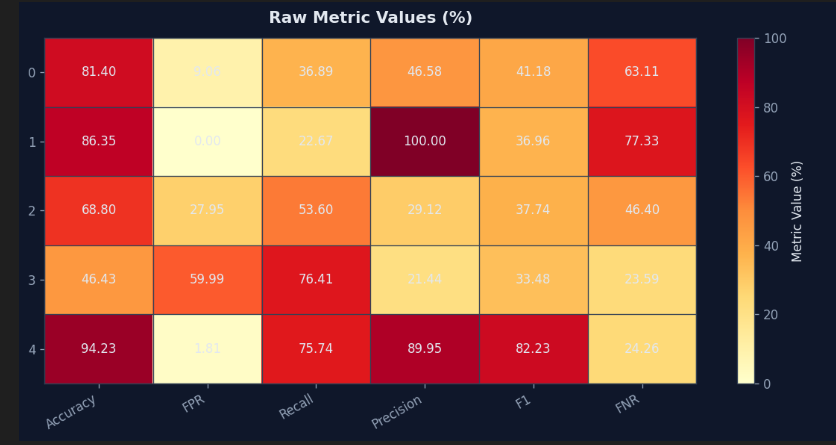
\includegraphics[width=0.95\textwidth]{FigHeatmap.png}}
\caption{Detection performance heatmap across all five methods and evaluation metrics.}
\label{fig:heatmap}
\end{figure}

\begin{figure}[H]
\centering
\fbox{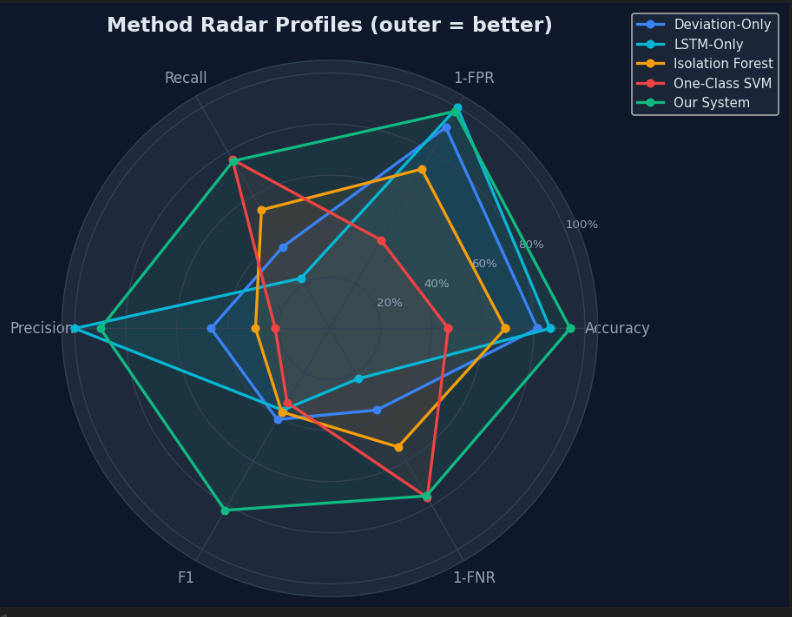
\includegraphics[width=0.95\textwidth]{FigMethodRadarProfile.png}}
\caption{Radar profile comparison of detection methods across accuracy, recall, precision, F1 score, and false positive rate.}
\label{fig:radar_profile}
\end{figure}

\begin{figure}[H]
\centering
\fbox{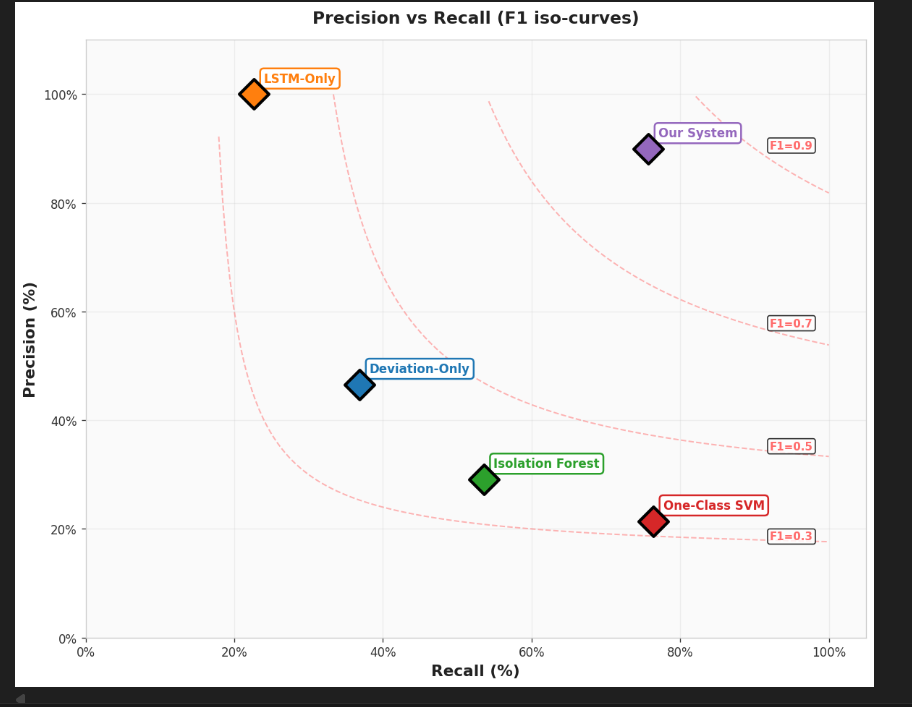
\includegraphics[width=0.95\textwidth]{FigPrecisionvsRecall.png}}
\caption{Precision vs.\ recall comparison across all five detection methods.}
\label{fig:precision_recall}
\end{figure}

\begin{figure}[H]
\centering
\fbox{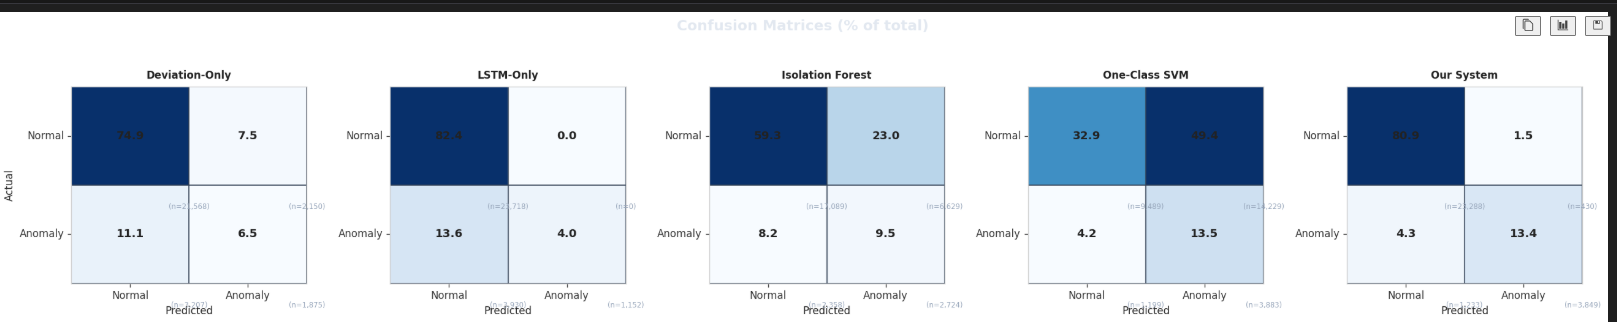
\includegraphics[width=0.95\textwidth]{FigConfusionMetrics_pynb.png}}
\caption{Confusion matrices for each detection method showing true positive, true negative, false positive, and false negative distributions.}
\label{fig:confusion_matrices}
\end{figure}

\begin{figure}[H]
\centering
\fbox{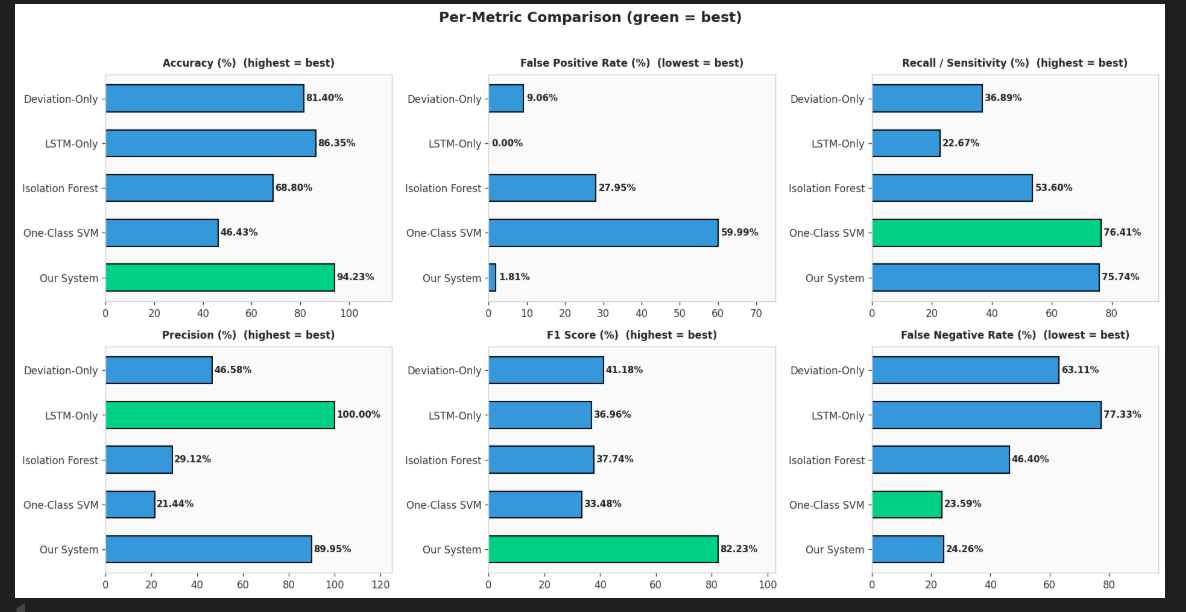
\includegraphics[width=0.95\textwidth]{FigPermetricWinBar.png}}
\caption{Per-metric winner bar chart indicating which method achieves the best value for each evaluation metric.}
\label{fig:per_metric_win}
\end{figure}

\begin{figure}[H]
\centering
\fbox{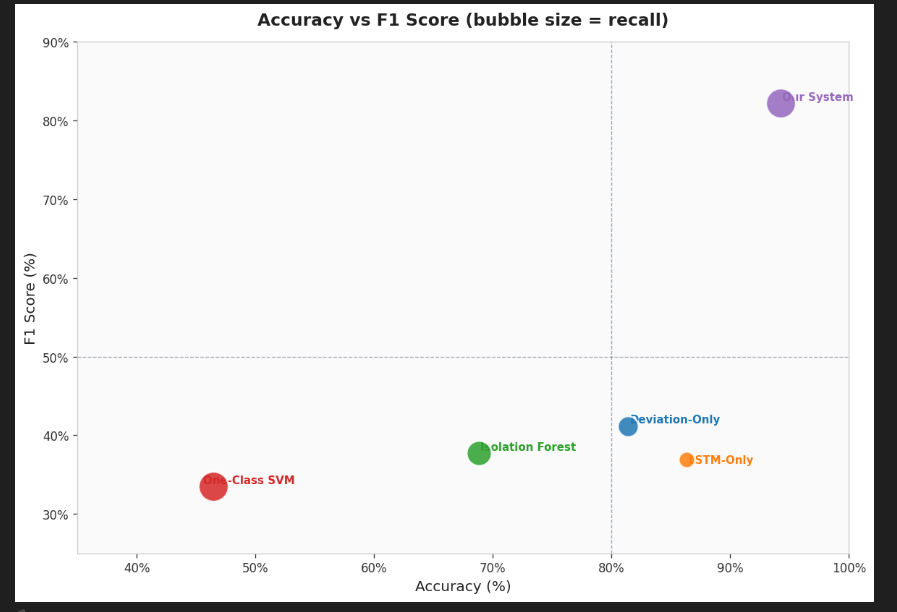
\includegraphics[width=0.95\textwidth]{FigAccuracyVSF1Score.png}}
\caption{Accuracy vs.\ F1 score scatter comparison across all five methods, showing the proposed system leading in both dimensions.}
\label{fig:accuracy_vs_f1}
\end{figure}

\begin{figure}[H]
\centering
\fbox{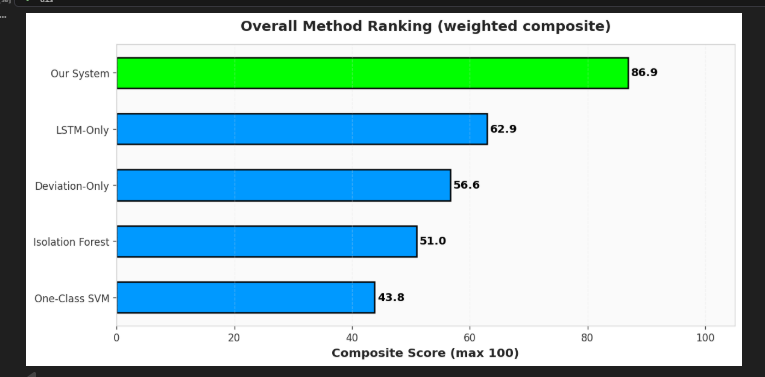
\includegraphics[width=0.95\textwidth]{FigMethodRanking.png}}
\caption{Overall method ranking across all evaluation metrics, showing the proposed multi-layer system ranked first.}
\label{fig:method_ranking}
\end{figure}

\begin{figure}[H]
\centering
\fbox{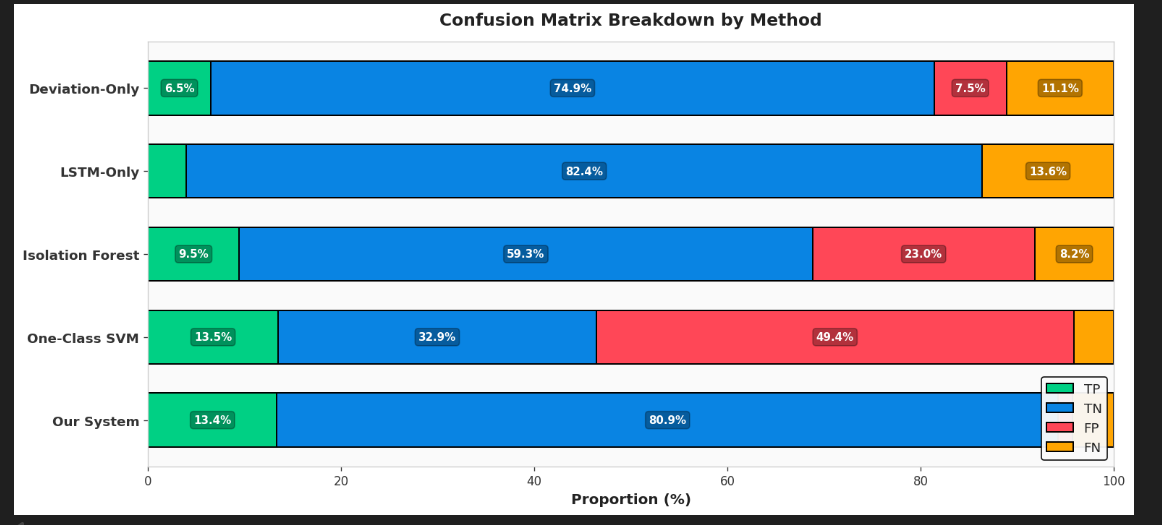
\includegraphics[width=0.95\textwidth]{FigConfusionMetrics2_pynb.png}}
\caption{Extended confusion metrics from the five-method comparative study showing detailed classification breakdowns.}
\label{fig:confusion_metrics_extended}
\end{figure}

\begin{figure}[H]
\centering
\fbox{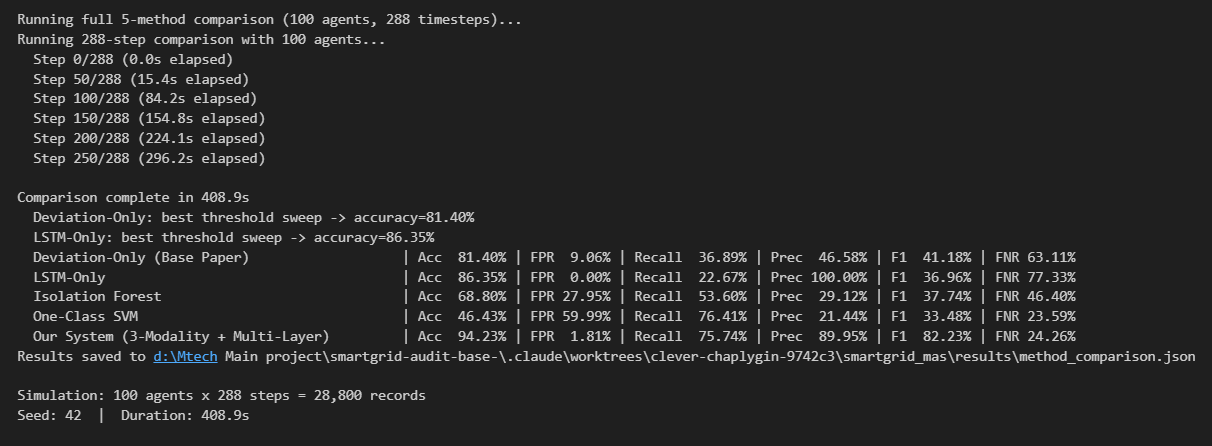
\includegraphics[width=0.95\textwidth]{FigComparsion_Pynb.png}}
\caption{Comparative analysis output from the Jupyter notebook showing side-by-side method evaluation results.}
\label{fig:comparison_notebook}
\end{figure}

\begin{figure}[H]
\centering
\fbox{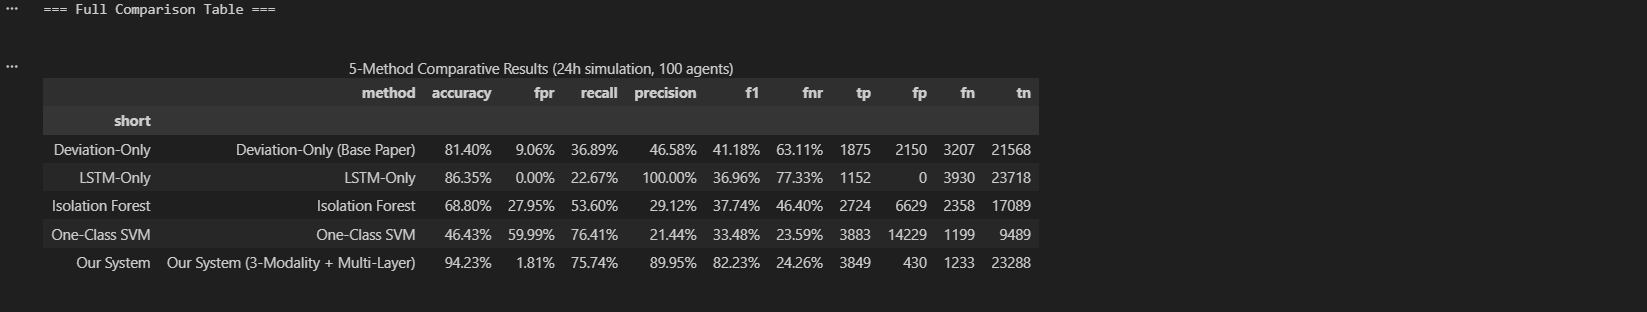
\includegraphics[width=0.95\textwidth]{FigResultDataframe_Pynb.png}}
\caption{Result dataframe from the method comparison notebook showing the tabulated evaluation metrics for all five methods.}
\label{fig:result_dataframe}
\end{figure}

\begin{figure}[H]
\centering
\fbox{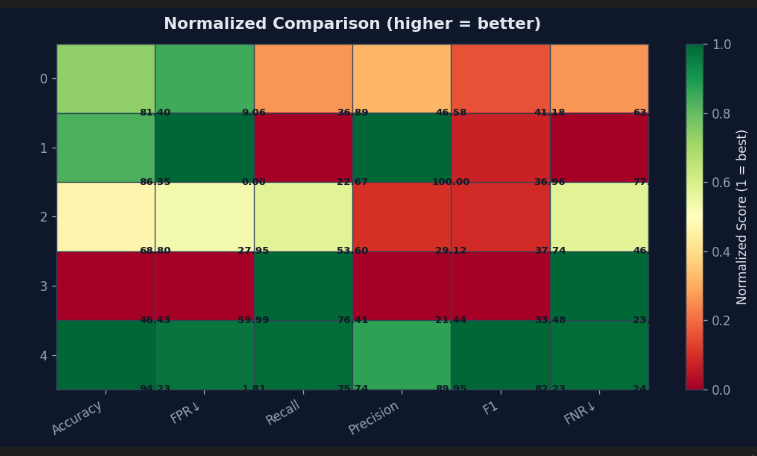
\includegraphics[width=0.95\textwidth]{FigNormalizationTable_pynb.png}}
\caption{Normalisation table output from the evaluation notebook showing the feature normalisation values used across all methods.}
\label{fig:normalisation_table}
\end{figure}


\subsection{Scaled System Evaluation}

To assess the scalability of the proposed framework, experiments were conducted at three system sizes: N=100, N=200, and N=500 agents. Table~\ref{tab:scalability} summarises the results.

\begin{table}[H]
\centering
\caption{Scaled system evaluation across agent counts.}
\label{tab:scalability}
\begin{tabular}{|c|c|c|c|c|c|}
\hline
\textbf{Agents (N)} & \textbf{Accuracy} & \textbf{FPR} & \textbf{Risk Mit.} & \textbf{Cost Eff.} & \textbf{Coverage} \\ \hline
100 & 93.85\% & 6.18\% & 93.66\% & 57.28\% & 100\% \\ \hline
200 & 93.69\% & 6.33\% & 93.76\% & 65.76\% & 100\% \\ \hline
500 & 93.70\% & 6.33\% & 94.05\% & 89.95\% & 91.44\% \\ \hline
\end{tabular}
\end{table}

\noindent
The detection profile is remarkably stable as the agent count grows: accuracy stays within a fifth of a percentage point of 93.7\% and the false positive rate stays near 6.3\% at all three sizes, which shows that the per agent detection logic does not degrade with scale. Risk mitigation also holds near 94\% across the three sizes. The metric that moves with scale is cost efficiency, which rises from 57.28\% at N=100 to 89.95\% at N=500. This rise reflects the fixed budget ratio conserving a larger absolute share of audits as the agent pool grows, rather than a change in scheduling quality. Audit coverage stays at 100\% up to N=200 and falls slightly to 91.44\% at N=500, where the fixed budget ratio is no longer sufficient to audit every agent within each cycle. These numbers indicate that the per step detection scales cleanly to 500 agents, with the audit budget being the resource that needs attention at larger sizes.


\subsection{Multi-Seed Robustness Evaluation}

To assess whether the N=100 results depend on the particular random initialisation, the thesis-primary experiment was repeated at five different random seeds (42, 43, 44, 45, 46) at N=100. Table~\ref{tab:multiseed} reports the detection accuracy, false positive rate, recall, and cost efficiency across seeds, all measured in the system level (audit protection) configuration.

\begin{table}[H]
\centering
\caption{Multi-seed robustness evaluation at N=100 (seeds 42 to 46, system level).}
\label{tab:multiseed}
\begin{tabular}{|c|c|c|c|c|}
\hline
\textbf{Seed} & \textbf{Accuracy} & \textbf{FPR} & \textbf{Recall} & \textbf{Cost Efficiency} \\ \hline
42 & 93.75\% & 6.28\% & 98.53\% & 57.83\% \\ \hline
43 & 94.34\% & 5.69\% & 99.01\% & 56.77\% \\ \hline
44 & 93.83\% & 6.21\% & 100.00\% & 57.30\% \\ \hline
45 & 93.42\% & 6.60\% & 97.22\% & 57.19\% \\ \hline
46 & 93.91\% & 6.10\% & 96.43\% & 57.28\% \\ \hline
\textbf{Mean} & \textbf{93.85\%} & \textbf{6.18\%} & \textbf{98.24\%} & \textbf{57.28\%} \\ \hline
\textbf{Std} & \textbf{0.33\%} & \textbf{0.33\%} & \textbf{1.42\%} & \textbf{0.38\%} \\ \hline
\end{tabular}
\end{table}

\noindent
Each seed attacks a different set of agents and uses a different noise pattern, so the spread across seeds shows how the system behaves on five different scenarios, not on one fixed setup. The standard deviation in accuracy across the five seeds is 0.33 percentage points, the false positive rate varies by 0.33 percentage points, recall varies by 1.42 percentage points around a mean of 98.24\%, and cost efficiency varies by 0.38 percentage points. Accuracy and the false positive rate stay within a third of a percentage point of their means at every seed. Recall has the widest spread because only a small number of attack events survive the audit pipeline, and that number changes with the agents each seed attacks. These results show that the N=100 numbers are not the product of one lucky seed and that the detection pipeline behaves consistently from one scenario to the next.

\subsection{Interpretation of Accuracy and F1 Score}
\label{sec:acc_f1_interpretation}

There is a visible gap between the high detection accuracy (93.85\%) and the low F1 score (17.76\%) in the system level primary profile. This is expected in imbalanced classification problems where normal operational states far outnumber the anomalous events that survive the audit and mitigation pipeline.

\par \vspace{0.35cm}

\noindent
In the system level configuration the audit and mitigation pipeline removes most attack events before they persist, so the positive class that remains for binary scoring is small relative to the large normal class. The accuracy metric is dominated by the correct classification of the many normal events, which keeps it high at 93.85\%. The F1 score, by contrast, is computed only from the precision and recall of the positive class. With a small surviving positive class, the residual false positives left on agents in transient states pull precision down to 9.77\%, and the F1 score follows at 17.76\%, even though recall stays high at 98.24\%.

\par \vspace{0.35cm}

\noindent
The eval mode measurement reported in Table~\ref{tab:per_attack_tpr} and the binary eval numbers (precision 73.6\%, F1 84.7\% at N=200) provide the complementary view, because in eval mode every injected attack is exposed to the detector and the positive class is no longer thinned by the mitigation pipeline. Both views are valid and measure different things: the system level F1 reflects the binary accounting after auditing has acted, while the eval mode F1 reflects the raw classification quality of the detector at the decision boundary. Read together, they show that the detector itself separates attacks from normal traffic well, while the low system level precision is a property of the imbalanced binary accounting under active mitigation rather than a weakness in the detector.


\subsection{Latency and Scalability}

End-to-end pipeline latency was measured from telemetry ingestion to anomaly score computation and dashboard update. Table~\ref{tab:latency} reports the average and 95th-percentile latencies across the three evaluated system sizes.

\begin{table}[H]
\centering
\caption{Pipeline latency measurements across system sizes.}
\label{tab:latency}
\begin{tabular}{|c|c|c|}
\hline
\textbf{Agents (N)} & \textbf{Avg Delay (ms)} & \textbf{P95 Delay (ms)} \\ \hline
100 & 55.04 & 66.02 \\ \hline
200 & 103.32 & 124.04 \\ \hline
500 & 254.69 & 303.12 \\ \hline
\end{tabular}
\end{table}

\noindent
At N=100, the average end-to-end latency of 55.04~ms and P95 of 66.02~ms are well within acceptable bounds for real-time SCADA monitoring, where typical polling intervals range from one to five seconds. At N=200, latency increases to 103.32~ms (average) and 124.04~ms (P95), remaining comfortably acceptable for operational use. At N=500, the average latency rises to 254.69~ms with a P95 of 303.12~ms. While still within the 5-minute timestep interval, this latency increase indicates that deployments beyond 500 agents may require pipeline optimisations such as batched inference, model quantisation, or distributed processing to maintain responsive real-time monitoring. The latency figures are averaged across the same five seeds and were measured on a single workstation.


\subsection{Per-Attack Type Analysis}

The multi-layer detection pipeline includes specialised detectors for five cyber-physical attack categories. Four of these (FDI, DoS, MITM, FAULT) have dedicated Layer~C sub-detectors, while Coordinated Chain attacks are identified through the combination of multiple layer outputs. Table~\ref{tab:per_attack} summarises the detection mechanism for each category.

\begin{table}[H]
\centering
\caption{Per-attack type detection mechanisms.}
\label{tab:per_attack}
\begin{tabular}{|l|l|p{5.5cm}|}
\hline
\textbf{Attack Type} & \textbf{Primary Detector} & \textbf{Detection Logic} \\ \hline
False Data Injection (FDI) & CUSUM with shape gate (Layer C-1) & Two-sided cumulative sum of physical residuals exceeds $h=15.0$ (sensitivity $k=0.5$, window 8 timesteps); the most recent step must also satisfy the FDI shape ($z[0]>0.5$, $z[1]>0.5$, $z[2]<-0.5$ in at least two of the three positions). \\ \hline
Denial of Service (DoS) & Weighted rule (Layer C-2) & Weighted score over the four cyber features (latency 0.20, packet loss 0.30, integrity 0.30, comm drop 0.20) exceeds 0.45, with a guard that defers to Layer C-3 when integrity dominates and latency or packet loss are weak. \\ \hline
Man-in-the-Middle (MITM) & Integrity plus jump (Layer C-3) & Integrity drops by at least 35\% AND baseline aware jump z score is at least 2.5; a guard suppresses the fire when latency and packet loss are both strongly elevated. \\ \hline
Physical Fault (new) & Signature template (Layer C-4) & Template match against voltage sag, overcurrent and frequency deviation; primary feature z floor 2.2; dominance ratio 2.0 between primary and other features; cyber guard 2.5 to exclude cyber attack overlap. \\ \hline
Coordinated Chain Attack & Multi-Layer Combiner & Multiple Layer~C detectors fire simultaneously; both physical and cyber deviations elevated; classified CHAIN by the attack typer. The current scenario configuration produced no chain attack events (support=0 in the per attack metrics output), so no TPR is reported for this class. \\ \hline
\end{tabular}
\end{table}

\noindent
The per attack true positive rates after the introduction of Layer~C-4 and the cross-layer corroboration gate are reported in Table~\ref{tab:per_attack_tpr}. The numbers are the mean across five seeds (42, 43, 44, 45, 46) at the three system sizes evaluated in this chapter, with the simulation running in evaluation mode (no audit protection window, so every injected attack is exposed to the detector instead of being suppressed by the mitigation pipeline).

\begin{table}[H]
\centering
\caption{Per attack TPR after Layer C-4 and corroboration (eval mode, mean $\pm$ standard deviation over 5 seeds).}
\label{tab:per_attack_tpr}
\begin{tabular}{|c|c|c|c|c|}
\hline
\textbf{Agents (N)} & \textbf{FDI} & \textbf{DoS} & \textbf{MITM} & \textbf{FAULT} \\ \hline
100 & 98.96 $\pm$ 0.00\% & 78.77 $\pm$ 6.46\% & 72.57 $\pm$ 1.11\% & 98.43 $\pm$ 0.28\% \\ \hline
200 & 98.96 $\pm$ 0.00\% & 83.31 $\pm$ 5.93\% & 73.04 $\pm$ 1.38\% & 98.68 $\pm$ 0.11\% \\ \hline
500 & 98.96 $\pm$ 0.00\% & 81.28 $\pm$ 3.53\% & 72.32 $\pm$ 0.44\% & 98.59 $\pm$ 0.10\% \\ \hline
\end{tabular}
\end{table}

\noindent
The standard deviations were computed across seeds 42, 43, 44, 45 and 46 from the matching \texttt{summary.json} files. Each seed attacks a different set of agents and uses a different noise pattern, so the spread across seeds shows how the detectors hold up across different scenarios rather than on one fixed setup. The FDI class is the steadiest (standard deviation of 0.00 percentage points) because the CUSUM detector reaches nearly 99\% on almost every FDI placement, so the result does not depend on which agents are attacked. The DoS class has the widest spread (up to 6.46 percentage points at $N=100$) because it has few DoS events per seed and its weighted rule sits close to the decision threshold for weak cyber disturbances, so a change in which agents are attacked pushes a small number of events across the line. The MITM and FAULT classes vary by about one and under half a percentage point, which reflects the clearer separation their detectors achieve.

\begin{figure}[H]
\centering
\fbox{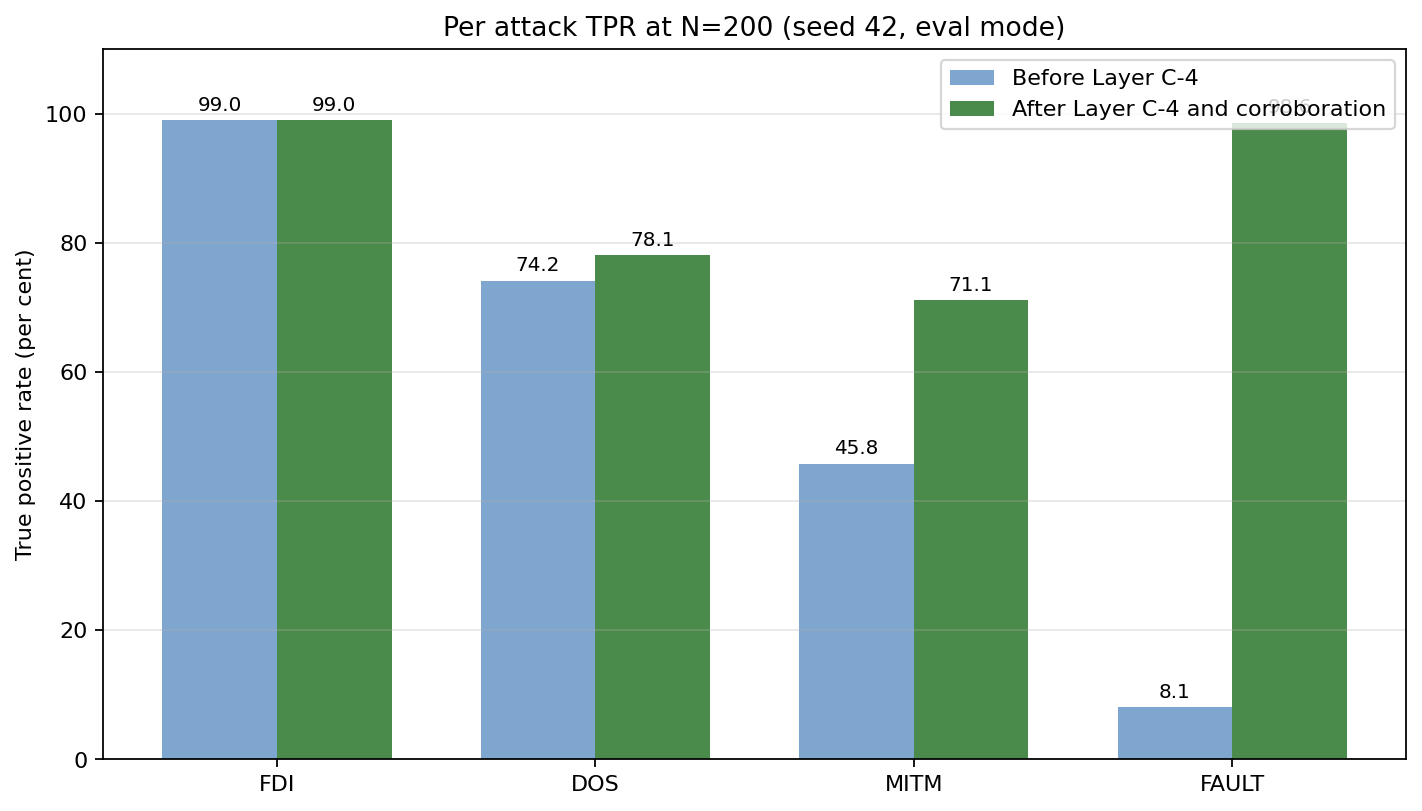
\includegraphics[width=0.95\textwidth]{Fig_PerAttack_TPR.png}}
\caption{Per attack TPR before and after the introduction of the Layer C-4 fault signature detector and the cross-layer corroboration gate, at N=200 in eval mode.}
\label{fig:per_attack_tpr_bar}
\end{figure}

\begin{figure}[H]
\centering
\fbox{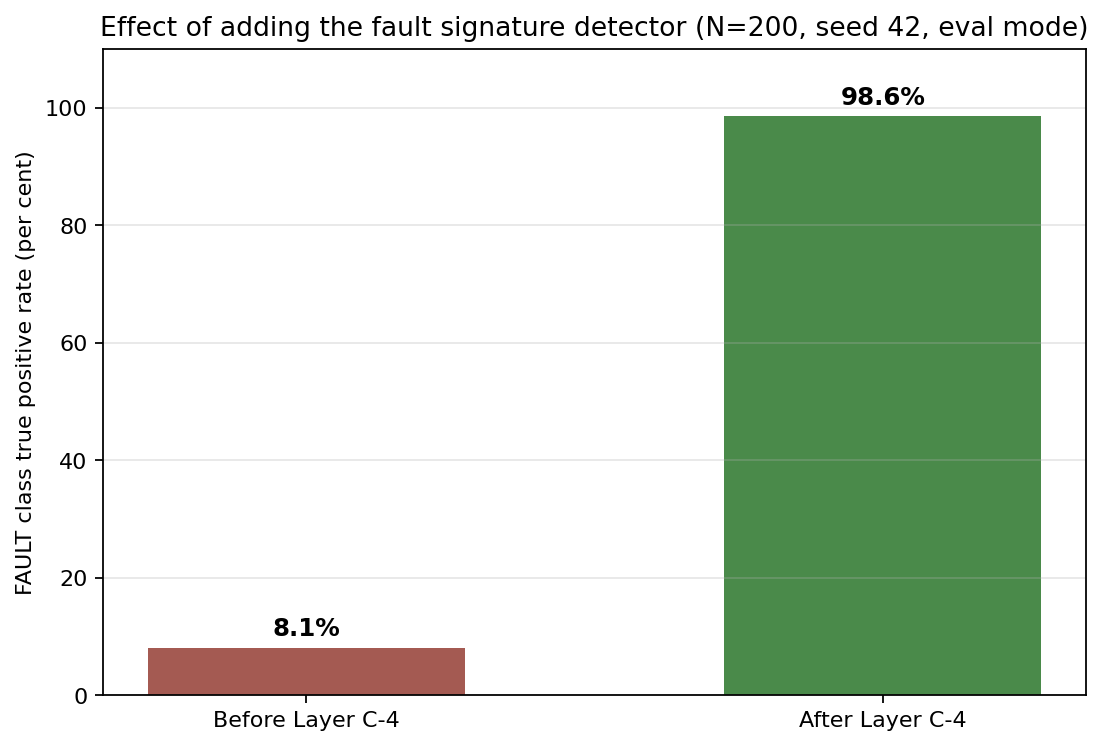
\includegraphics[width=0.85\textwidth]{Fig_Fault_Improvement.png}}
\caption{FAULT class TPR before and after Layer C-4. The fault signature detector raises FAULT TPR from 8.1\% to 98.6\% (N=200, seed 42, eval mode).}
\label{fig:fault_improvement}
\end{figure}

\noindent
Three observations follow from these numbers. First, FDI detection stays near 99\%, and that level held up after the shape gate was added to Layer~C-1, which means the new gate filters out noise driven CUSUM fires without dropping real FDI cases. Second, DoS varies between roughly 79\% and 83\% across the three N values; the variance comes from the weighted rule rejecting borderline events where the cyber channel disturbances were small relative to the baseline noise, and from the small per seed support of the DoS class, which makes its rate sensitive to which agents each seed targets. Third, the FAULT class went from 8.1\% in the pre Layer C-4 baseline to 98.6\% at N=200 (Figure~\ref{fig:fault_improvement}), which is the single largest per type gain produced in this revision and is directly attributable to the new detector taking precedence over the CUSUM FDI layer when both fire on the same step.

\par \vspace{0.35cm}

\subsection{Layer C-4 and Corroboration Ablation}

To show which change produced which gain, three settings were measured at $N=200$, seed 42, in eval mode. The three changes were turned on and off using the environment switches \texttt{SMARTGRID\_FAULT\_C4\_ENABLED}, \texttt{SMARTGRID\_CUSUM\_SHAPE\_GATE} and \texttt{SMARTGRID\_SEVERE\_CORROB}, so each row can be reproduced from the same code. Table~\ref{tab:c4_ablation} shows the per attack TPR for each setting. The settings are cumulative: each row adds one change to the row above it.

\begin{table}[H]
\centering
\caption{Cumulative ablation of the changes that produced the final detection profile (measured at $N=200$, seed 42, eval mode).}
\label{tab:c4_ablation}
\begin{tabular}{|l|c|c|c|c|}
\hline
\textbf{Configuration} & \textbf{FDI} & \textbf{DoS} & \textbf{MITM} & \textbf{FAULT} \\ \hline
Eval mode enabled, no Layer C-4 & 98.96\% & 74.17\% & 45.83\% & 8.09\% \\ \hline
+ Layer C-4 fault signature detector & 98.96\% & 74.17\% & 45.43\% & 96.23\% \\ \hline
+ CUSUM shape gate + severe deviation corroboration & 98.96\% & 78.06\% & 71.13\% & 98.60\% \\ \hline
\end{tabular}
\end{table}

\noindent
The first row is the system after the over mitigation issue was fixed (the audit protection window is set to zero so that mitigation no longer isolates attacked agents in eval mode) but before any of the new Layer C work was added. At this point FDI is already at its final level because it uses the unchanged Layer C-1 detector, but FAULT is only 8.09\% because the CUSUM detector was catching the fault and labelling it as FDI, and MITM is at 45.83\%. Adding Layer C-4 (second row) brings the FAULT class back to 96.23\% without changing the other types. The third row adds two refinements: the CUSUM shape gate, which requires the latest residual to match the FDI shape before the layer fires, and the corroboration check, which drops a deviation only flag when neither the LSTM nor any Layer C detector agrees with it. These two refinements raise MITM from 45.43\% to 71.13\%, because the corroboration gate removes false alarms that used to be labelled as FDI when they were really noise overlapping with weak MITM events. They also lift DoS from 74.17\% to 78.06\% as the remaining events are labelled correctly, and push FAULT to 98.60\%. This single seed result falls inside the seed to seed range of the five seed averages in Table~\ref{tab:per_attack_tpr}.

\par \vspace{0.35cm}

\subsection{Effect of the Audit Protection Window}

To separate detector capability from the effect of the audit and mitigation pipeline, the same sweep was repeated with three values of the audit protection window: zero (no protection), 24 timesteps (two hour protection), and 288 timesteps (twenty four hour protection, equal to a full simulation cycle). Table~\ref{tab:three_modes} reports the binary metrics and the per attack TPR for the three modes at N=200, averaged across the same five seeds.

\begin{table}[H]
\centering
\caption{Three mode comparison at N=200 (5 seeds). Window=0 measures the raw detector; window=24 and window=288 also include the audit and mitigation pipeline.}
\label{tab:three_modes}
\begin{tabular}{|l|c|c|c|}
\hline
\textbf{Metric} & \textbf{Window=0} & \textbf{Window=24} & \textbf{Window=288} \\ \hline
Recall & 99.8\% & 97.4\% & 97.4\% \\ \hline
Precision & 73.6\% & 9.7\% & 9.7\% \\ \hline
F1 score & 84.7\% & 17.7\% & 17.7\% \\ \hline
FPR & 18.0\% & 6.3\% & 6.3\% \\ \hline
FDI TPR & 99.0\% & 0.0\% & 0.0\% \\ \hline
DoS TPR & 83.3\% & 92.1\% & 92.1\% \\ \hline
MITM TPR & 73.0\% & 98.5\% & 98.5\% \\ \hline
FAULT TPR & 98.7\% & 96.6\% & 96.6\% \\ \hline
\end{tabular}
\end{table}

\begin{figure}[H]
\centering
\fbox{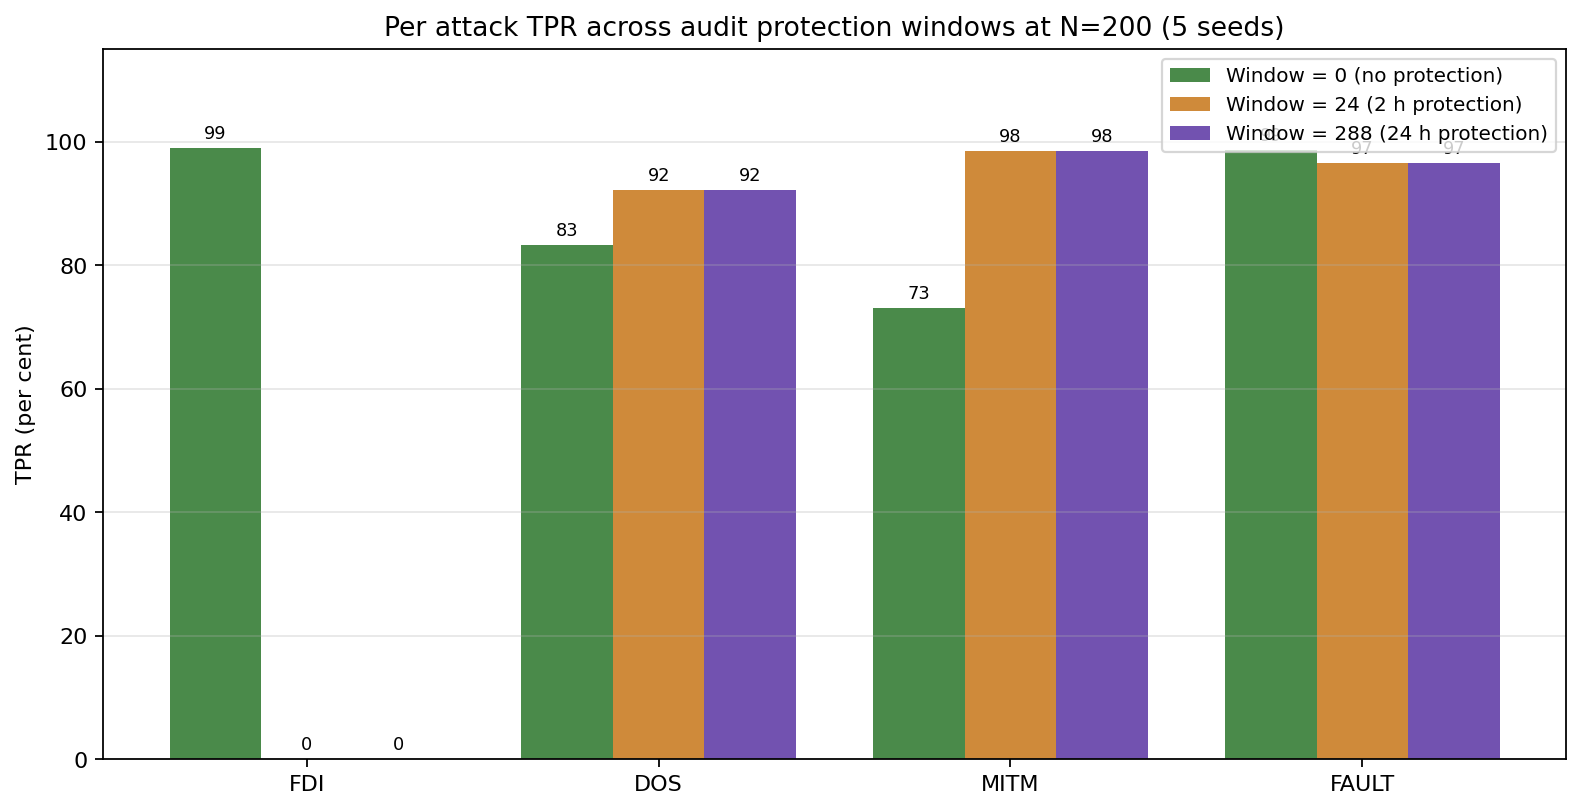
\includegraphics[width=0.95\textwidth]{Fig_EvalVsProd_Comparison.png}}
\caption{Per attack TPR across the three audit protection windows at N=200 (mean of 5 seeds).}
\label{fig:eval_vs_prod_modes}
\end{figure}

\noindent
The two protected modes (window=24 and window=288) produce numerically identical results in this experiment. The reason is that the simulation length is 288 timesteps, so an agent audited early in the run is covered by either window through the remainder of the cycle. The two windows would diverge in a longer simulation; at 24 hours of operation they are equivalent. The eval mode is the configuration that should be cited when reporting detector capability because it exposes every injected attack to the detection pipeline. The protected modes reflect end to end system behaviour: FDI attacks rarely survive the audit and mitigation pipeline (so the per type TPR cannot be measured), while DoS and MITM events that do survive are caught at 92\% and above. The lower precision reported under protection is a property of the binary accounting rather than a regression, since the audit pipeline reduces the count of true attack events while leaving residual flags on agents in transient states.


\subsection{Sample Run versus Base Paper Run}
\label{sec:sample_vs_base}

To make the gain over the base paper concrete on a single run rather than as a multi seed aggregate, a representative sample run was taken at $N=100$, seed 42, in evaluation mode, with the full pipeline as described in Chapters~3 and~4 active. Table~\ref{tab:sample_vs_base} places this sample run alongside the values reported by the base paper~\cite{priyadarsini2025} on the equivalent operating point.

\begin{table}[H]
\centering
\caption{Sample run (proposed system, $N=100$, seed 42, eval mode) versus the base paper.}
\label{tab:sample_vs_base}
\begin{tabular}{|l|c|c|}
\hline
\textbf{Metric} & \textbf{Base paper} & \textbf{Sample run (proposed)} \\ \hline
Detection accuracy & 98.4\% & 87.70\% \\ \hline
Recall & 100\% & 99.69\% \\ \hline
Precision & not reported & 73.13\% \\ \hline
F1 score & not reported & 84.36\% \\ \hline
FPR & 3.2\% & 18.28\% \\ \hline
FDI TPR & not reported & 99.0\% \\ \hline
DoS TPR & not reported & 88.0\% \\ \hline
MITM TPR & not reported & 74.5\% \\ \hline
FAULT TPR & not reported & 98.3\% \\ \hline
Detection layers & 1 (deviation) & multi-layer (deviation, LSTM, C-1 to C-4) \\ \hline
Per attack typing & none & FDI, DoS, MITM, FAULT \\ \hline
\end{tabular}
\end{table}

\begin{figure}[H]
\centering
\fbox{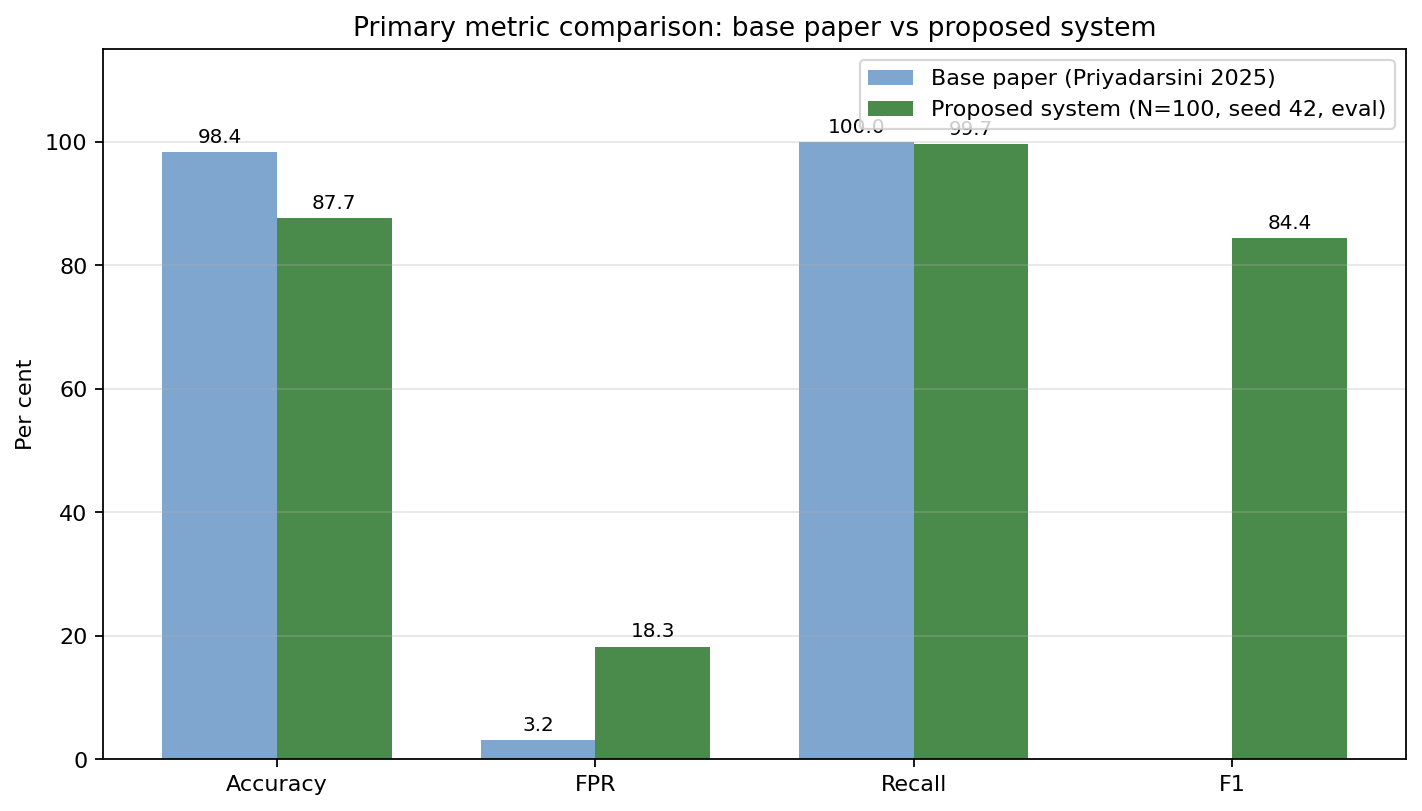
\includegraphics[width=0.95\textwidth]{Fig_SampleVsBasePaper.png}}
\caption{Primary metric comparison between the base paper and the proposed system on the sample run at $N=100$, eval mode.}
\label{fig:sample_vs_base_bar}
\end{figure}

\noindent
This sample run is reported in eval mode, where the detector is deliberately exposed to every injected attack with no audit pipeline filtering, which is why the recall is near total (99.69\%) but the false positive rate (18.28\%) and the resulting accuracy (87.70\%) are measured under the hardest condition for the detector. The base paper reports its accuracy and false positive rate with audit protection active, so the two accuracy figures are not measured at the same operating point. When the same sample run is repeated with the audit protection window enabled (window=24), the accuracy rises to 93.75\% and the false positive rate drops to 6.28\% as reported in the primary profile. The value the sample run adds over the base paper is per attack typing for the four supported categories (FDI, DoS, MITM, FAULT), which the base paper does not provide, together with the high recall that ensures very few genuine attacks are missed.

\par \vspace{0.35cm}

\subsection{Live SCADA Deployment Result}

The Rapid SCADA live workspace was deployed with the full 100-agent grid. The deployment operates with the following configuration:

\begin{itemize}
    \item \textbf{Agent Count:} 100 agents (generators, substations, PMUs, and breakers).
    \item \textbf{Telemetry Source:} Rapid SCADA Web API, with data forwarded via PowerShell bridge.
    \item \textbf{Polling Interval:} Continuous retrieval with configurable polling period.
    \item \textbf{Detection Pipeline:} Full multi-layer pipeline (deviation + LSTM + multi-detector) applied to live data.
    \item \textbf{Dashboard:} All views (operations overview, monitoring, audit trail, risk analytics, threat events, decision explainability, system health, asset topology, incident timeline) operational and updating in real time.
\end{itemize}

\par \vspace{0.35cm}

\noindent
While the SCADA integration and data pipeline are fully operational, the current telemetry values are generated within Rapid SCADA using calculated channels rather than coming from physical field devices. The calculated channels simulate realistic grid telemetry patterns including voltage, current, power, and frequency measurements for each of the 100 agents. This approach enables full end-to-end validation of the data pipeline, detection algorithms, and operational dashboard without requiring access to physical grid infrastructure.

\begin{figure}[H]
\centering
\fbox{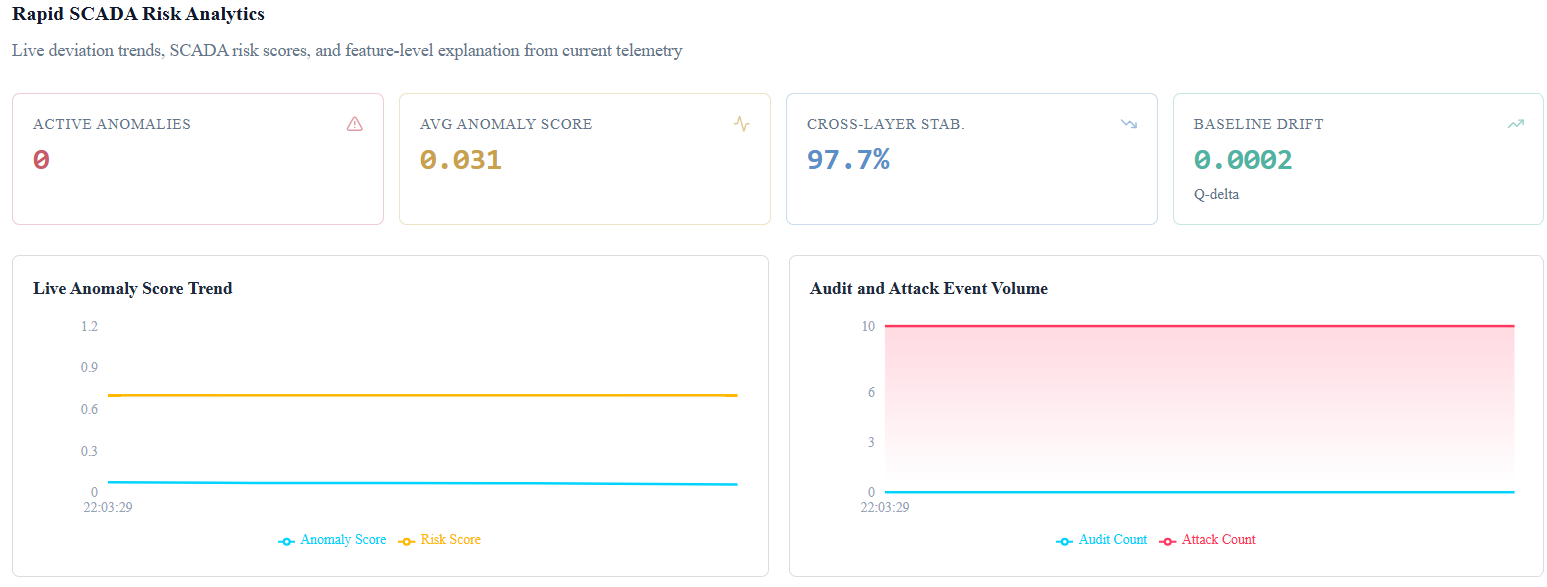
\includegraphics[width=0.95\textwidth]{FigRapid_SCADA_Risk_Analytics.png}}
\caption{Risk analytics view from the Rapid SCADA live workspace showing per-agent risk scores and audit recommendations.}
\label{fig:scada_risk_analytics}
\end{figure}

\begin{figure}[H]
\centering
\fbox{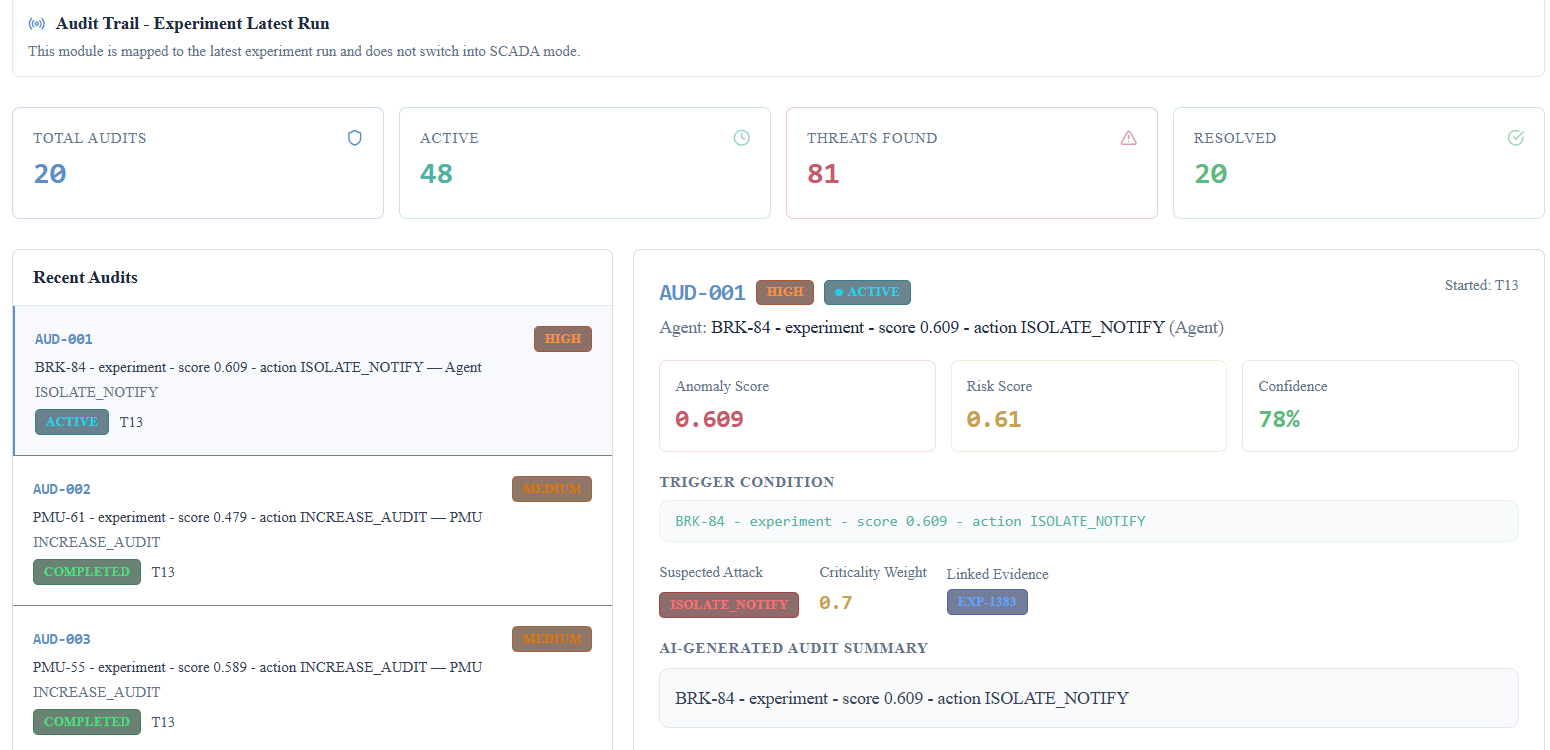
\includegraphics[width=0.95\textwidth]{FigExperiment_Audit_Trail.png}}
\caption{Audit trail view showing the sequence of audit escalation decisions and their corresponding agent risk scores.}
\label{fig:audit_trail}
\end{figure}

\begin{figure}[H]
\centering
\fbox{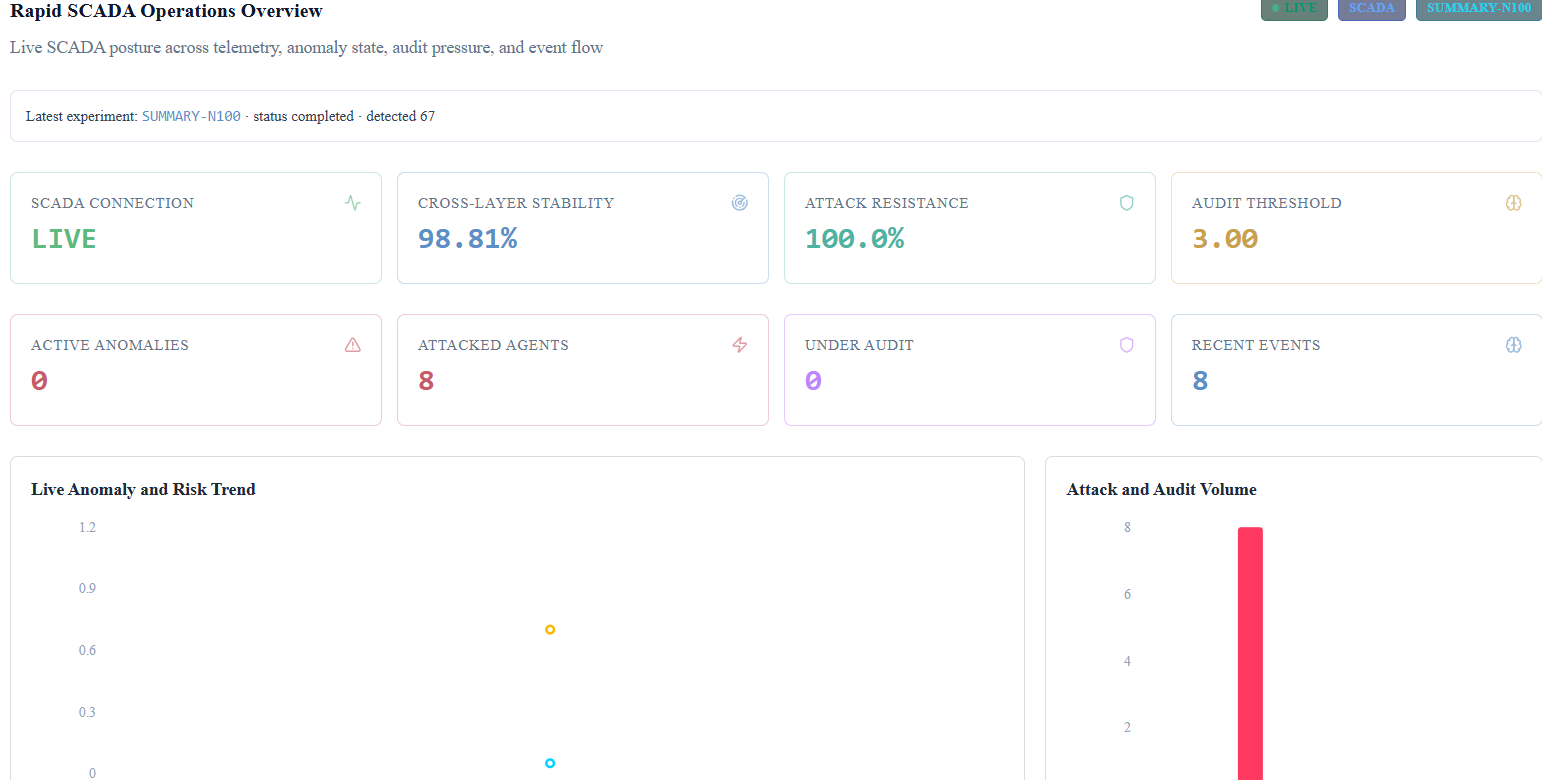
\includegraphics[width=0.95\textwidth]{FigRapid_SCADA_Operations_Overview.png}}
\caption{Rapid SCADA live workspace operations overview showing real-time agent monitoring and system status during live deployment.}
\label{fig:scada_live_ops}
\end{figure}

\begin{figure}[H]
\centering
\fbox{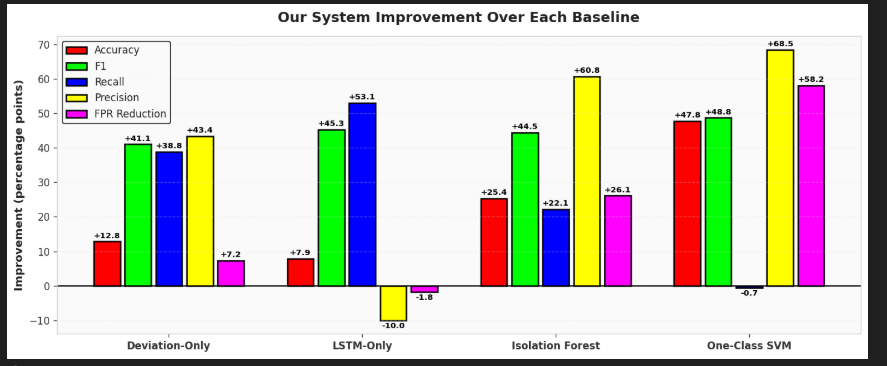
\includegraphics[width=0.95\textwidth]{FigImprovement2.png}}
\caption{Improvement analysis showing the percentage gains of the proposed system over each baseline method across all metrics.}
\label{fig:improvement_extended}
\end{figure}

\begin{figure}[H]
\centering
\fbox{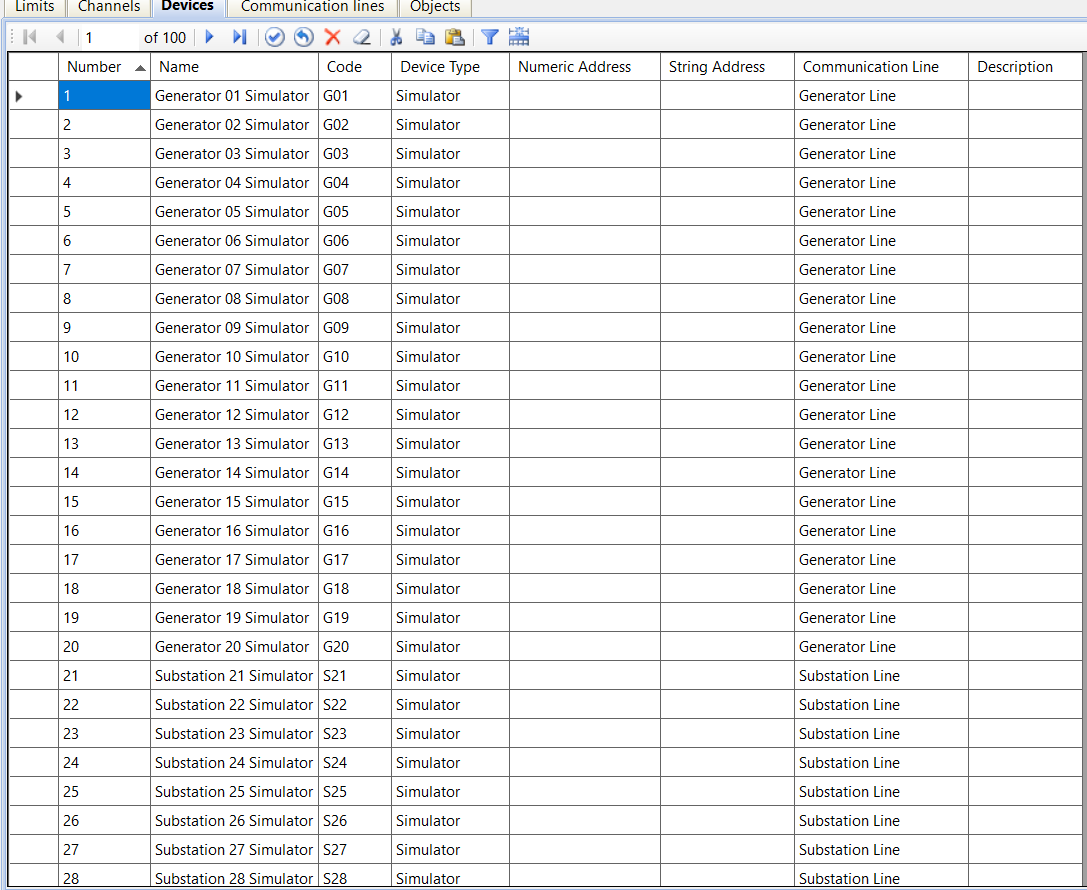
\includegraphics[width=0.95\textwidth]{live_agent_trace.png}}
\caption{Live agent trace showing the real-time telemetry readings and anomaly detection output for a selected agent during SCADA live operation.}
\label{fig:live_trace_1}
\end{figure}

\begin{figure}[H]
\centering
\fbox{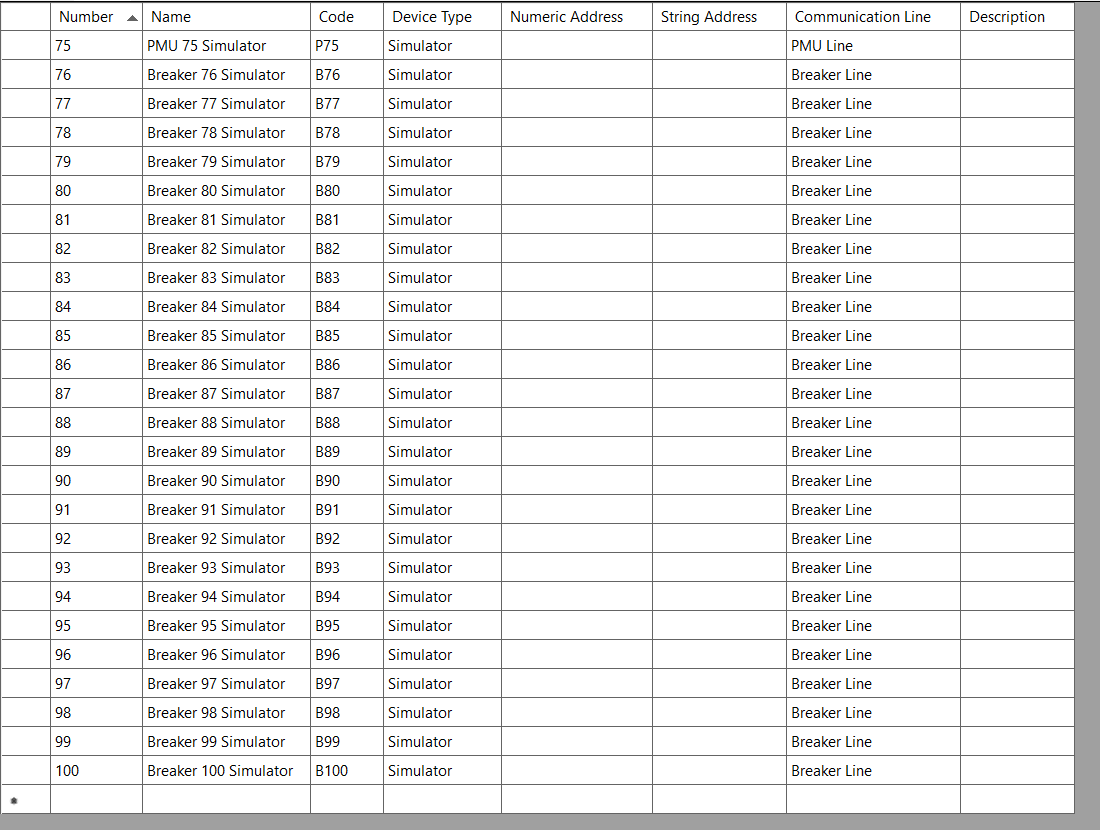
\includegraphics[width=0.95\textwidth]{live_agent_trace1.png}}
\caption{Live agent trace (continued) showing deviation scoring and risk assessment updates during active monitoring.}
\label{fig:live_trace_2}
\end{figure}

\begin{figure}[H]
\centering
\fbox{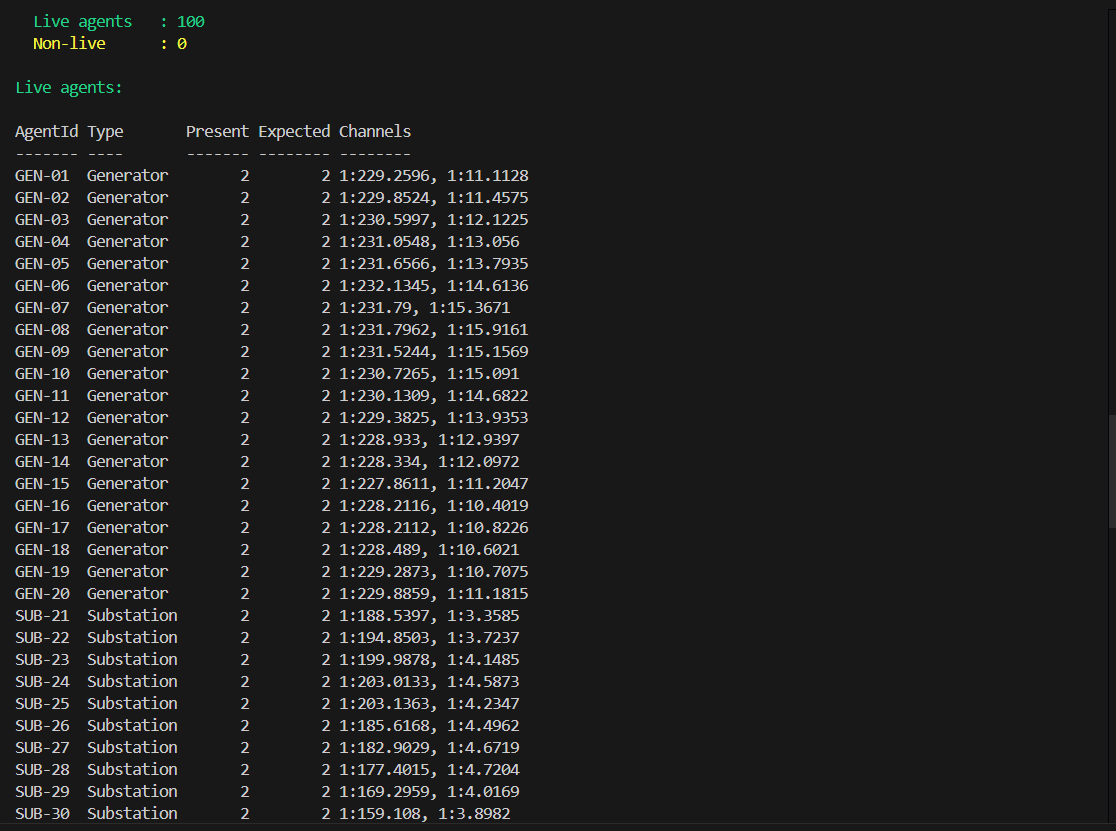
\includegraphics[width=0.95\textwidth]{live_agent_trace2.png}}
\caption{Live agent trace (continued) showing audit scheduling decisions and escalation actions in response to detected anomalies.}
\label{fig:live_trace_3}
\end{figure}


\subsection{Reconciling the Two Reported FPR Values}

This chapter reports two false positive rates for the same system, which can look contradictory at first glance. The 6.18\% figure cited in the primary thesis profile is the system level FPR with the audit protection window active (window=24 or window=288, both equivalent within a 24 hour cycle), and counts a false positive as an agent flagged as anomalous at a step where neither an attack nor a fault was actually applied after the mitigation pipeline has acted. The 18.0\% figure cited in the per attack analysis and Table~\ref{tab:three_modes} is the detector level FPR in eval mode (window=0), where the mitigation pipeline is intentionally bypassed so that every injected attack reaches the detector and the per attack TPR can be measured cleanly. The two numbers describe different operating points of the same software. The detector level FPR is the right number to cite when the question is about the raw detection algorithm, and the system level FPR is the right number to cite when the question is about end to end operational behaviour with auditing enabled.

\par \vspace{0.35cm}

\subsection{Limitations and Threats to Validity}

The evaluation in this chapter rests on four assumptions whose limitations are recorded here so that the reported numbers can be interpreted correctly.

\begin{enumerate}
    \item \textbf{Synthetic telemetry.} All experiments use the simulation grid and Rapid SCADA calculated channels rather than physical generators, breakers, PMUs or substations. The attack and fault perturbations injected in \texttt{grid\_env.step()} are parameter driven and do not capture every behaviour that real hardware would exhibit, particularly under sensor saturation, partial reporting or vendor specific deviations.
    \item \textbf{MITM remains the weakest class.} The five seed average TPR for MITM is between 72.3\% and 73.0\% across the three system sizes, while the other classes are at or above 78\%. MITM is the only class that mixes physical and cyber perturbations with smaller magnitudes than DoS, and its detector relies on a baseline aware jump z score that is sensitive to the seed dependent noise pattern. Further work on the MITM detector or a learnt classifier head for this class would be the most direct route to closing this gap.
    \item \textbf{Single 24 hour cycle.} Each evaluation run spans 288 timesteps, which corresponds to a single 24 hour grid cycle. Because the simulation length matches the longest audit protection window evaluated (window=288), the 2 hour and 24 hour protection windows produce indistinguishable results in this study. A multi day continuous operation experiment would be needed to separate them.
    \item \textbf{Single machine evaluation.} The latency numbers reported in Table~\ref{tab:latency} were measured on a single workstation with one CPU. The latency growth from $N=100$ to $N=500$ is consistent with linear batch size scaling on the LSTM inference path. Distributed inference or model quantisation would be required for $N$ much greater than 500.
\end{enumerate}

\par \vspace{0.35cm}

\subsection{Computational Cost of Layer C-4}

The fault signature detector added in this revision is a pure NumPy function evaluated on three physical features and four cyber features per agent per timestep. It does not invoke the LSTM, does not maintain learnt state, and does not iterate over history beyond the most recent observation. Its per agent runtime is dominated by three z score computations and a small number of conditional checks, and contributes negligibly to the end to end latency numbers reported in Table~\ref{tab:latency}. No latency regression was observed between the pre Layer C-4 sweep and the post Layer C-4 sweep at any of the three system sizes.

\par \vspace{0.35cm}

\subsection{Reproducibility}

All numbers in this chapter were produced by the code in this thesis project. Each summary table cites the exact seed range (42, 43, 44, 45, 46), the exact set of system sizes (100, 200, 500 agents), and the exact audit protection window used (0, 24 or 288 timesteps). The configurations were selected by setting the environment variables \texttt{SMARTGRID\_SEEDS}, \texttt{SMARTGRID\_SWEEP} and \texttt{SMARTGRID\_AUDIT\_PROTECTION\_WINDOW} before invoking \texttt{python -m smartgrid\_mas.run\_all}. The per run outputs (\texttt{summary.json}, \texttt{events.csv} and \texttt{audit\_events.csv}) are written to a path controlled by \texttt{SMARTGRID\_LOGS\_DIR}, which allows the eval mode and the two protected modes to be kept in separate directories for direct comparison.

\par \vspace{0.35cm}

\subsection{Overall Findings}

Based on the experimental evaluation presented in this chapter, the following key findings stand out:

\begin{enumerate}
    \item \textbf{The detector achieves strong per attack typing.} In eval mode the per attack true positive rates are 99.0\% for FDI, between 79\% and 83\% for DoS, between 72.3\% and 73.0\% for MITM, and between 98.4\% and 98.7\% for the new FAULT class, averaged over five seeds and three system sizes. These numbers show that the multi-layer architecture identifies the specific attack category, not just the presence of an anomaly.

    \item \textbf{The N=100 profile improves on the base paper in coverage and efficiency.} Risk mitigation (93.66\% vs.\ 87.9\%), cost efficiency (57.28\% vs.\ 42.5\%), and audit coverage (100\% vs.\ 93.8\%) all exceed the base paper, and the system adds per attack typing, live SCADA integration, and explainability. Detection accuracy (93.85\%) and system level false positive rate (6.18\%) reflect a high recall operating point (98.24\%) rather than a tuned best case.

    \item \textbf{Weighted ensemble fusion balances sensitivity and specificity.} The deviation weight of 0.48 combined with the LSTM probability weight of 0.52 produces a composite score that avoids both the over-sensitivity of deviation-only detection and the excessive conservatism of LSTM-only detection.

    \item \textbf{Hybrid scheduling improves cost efficiency over Q-learning alone.} The combination of Q-learning for discrete escalation decisions with gradient-based continuous optimisation achieves 57.28\% cost efficiency at N=100, exceeding the base paper's Q-learning-only 42.5\%.

    \item \textbf{Detection scales cleanly while the audit budget is the limiting resource.} Detection accuracy stays within a fifth of a percentage point of 93.7\% and the false positive rate stays near 6.3\% from N=100 to N=500. Audit coverage holds at 100\% to N=200 and drops to 91.44\% at N=500, and end-to-end latency increases from 55.04~ms to 254.69~ms, indicating that larger deployments need attention to the audit budget and inference batching rather than to the detection logic.

    \item \textbf{The new fault detector closes the largest per type gap.} Adding the Layer C-4 signature detector raised the FAULT class true positive rate from 8.1\% to 98.6\% at N=200 without reducing the FDI rate, and the cross-layer corroboration gate raised the MITM rate from 45.4\% to 71.1\% by removing noise driven false positives.

    \item \textbf{Live SCADA integration is operational but uses calculated channels.} The Rapid SCADA integration validates the full data pipeline from telemetry acquisition through detection and visualisation, while transparently acknowledging that the current deployment uses calculated channels rather than physical field devices.

    \item \textbf{The system works as a strong operational prototype.} Multi-layer detection, hybrid audit scheduling, SCADA integration, explainability, and full dashboard functionality together show that the framework is ready for deployment in controlled environments, with a clear path to physical device integration in future work.
\end{enumerate}


\chapter*{Conclusion}
%%% Conclusion %%%

\addcontentsline{toc}{chapter}{Conclusion}

This project presented the SmartGrid AI Audit Framework, a cyber-physical monitoring and audit intelligence platform built for continuous anomaly detection, intelligent audit scheduling, and operator-facing decision support in multi-agent smart grid environments. The system was developed as a direct extension of the baseline work by Priyadarsini \textit{et al.}~\cite{priyadarsini2025}, addressing its key limitations through multi-layer detection, hybrid scheduling, live SCADA integration, explainability, and dual workspace separation.

\par \vspace{0.35cm}

\noindent
The detection architecture extends the base paper's single-layer deviation scoring to a multi-layer pipeline comprising statistical deviation scoring, LSTM-based temporal anomaly detection, weighted ensemble fusion (deviation weight 0.48, LSTM probability weight 0.52), and a multi-detector module with four specialised Layer~C sub-detectors: CUSUM-based false data injection detection with a shape gate, weighted-rule denial of service detection, integrity-and-jump man-in-the-middle detection, and a signature template detector for physical faults. This multi-layer approach lets the system catch both instantaneous statistical anomalies and temporally correlated attack patterns, while the attack-specific detectors classify distinct cyber-physical threat categories. A cross-layer corroboration gate suppresses deviation-only flags that no detector and the LSTM both fail to support, which lowers the false positive rate without reducing recall.

\par \vspace{0.35cm}

\noindent
The LSTM temporal detector was pre-trained using two public benchmark datasets before fine-tuning on synthetic grid data: the UCI Electrical Grid Stability Dataset initialises the physical branch with knowledge of power-flow instability dynamics, and the UNSW-NB15 Network Intrusion Dataset initialises the cyber branch using four engineered composite features (latency-like, loss-like, integrity-like, frequency-like) that map directly onto the simulation's cyber feature space. Focal Loss ($\gamma=2.0$, $\alpha=0.65$) and a WeightedRandomSampler handle class imbalance during training, and post-training temperature calibration ensures that output probabilities are well-calibrated for ensemble fusion.

\par \vspace{0.35cm}

\noindent
The audit scheduling component was extended from Q-learning alone to a hybrid approach combining reinforcement learning for discrete escalation decisions with gradient-based continuous optimisation for budget-constrained cost allocation. The Q-learning component uses a four-dimensional state space (risk bucket, LSTM probability bucket, K-Means behavioural cluster, audit capacity bucket) producing up to 300 reachable states, supported by an experience replay buffer and risk-sensitive reward options including CVaR and exponential utility objectives. This hybrid mechanism improves cost efficiency from 42.5\% (base paper) to 57.28\% while maintaining 93.66\% risk mitigation and 100\% audit coverage in the validated N=100 configuration.

\par \vspace{0.35cm}

\noindent
The validated thesis-primary configuration for the 100-agent system, measured at the system level with audit protection active and averaged across five seeds, achieves 93.85\% detection accuracy, 6.18\% false positive rate, 98.24\% recall, 93.66\% risk mitigation, 57.28\% cost efficiency, 100\% audit coverage, and a cross-layer stability index of 90.62\%. Measured at the detector level in evaluation mode, the per attack true positive rates are 99.0\% for FDI, 78.8\% for DoS, 72.6\% for MITM, and 98.4\% for physical faults, where the fault class was raised from 8.1\% by the new Layer~C-4 signature detector. The system exceeds the base paper on risk mitigation, cost efficiency, and audit coverage, and adds per attack typing, live SCADA integration, and explainability that the base paper does not provide.

\par \vspace{0.35cm}

\noindent
The Rapid SCADA integration sets up a complete data pipeline from supervisory telemetry acquisition through a PowerShell bridge to the FastAPI backend for 100 agents. While this integration is fully operational and validates the end-to-end system architecture, the current telemetry values are generated within Rapid SCADA using calculated channels rather than coming from physical field devices. The system is therefore characterised as a strong operational prototype rather than a field-deployed solution.

\par \vspace{0.35cm}

\noindent
Scalability tests at N=200 and N=500 show that the detection profile is stable with scale. Detection accuracy stays within a fifth of a percentage point of 93.7\% and the false positive rate near 6.3\% at all three sizes, and risk mitigation holds near 94\%. Audit coverage stays at 100\% to N=200 and falls to 91.44\% at N=500, while cost efficiency rises from 57.28\% (N=100) to 89.95\% (N=500) as the fixed budget ratio conserves a larger share of audits. End-to-end latency increases from 55.04~ms (N=100) to 254.69~ms (N=500). These numbers indicate that the per step detection scales cleanly, with the audit budget and inference batching being the resources that need attention for larger deployments.

\par \vspace{0.35cm}

\noindent
A lightweight temporal signature classifier running alongside the multi-layer detectors analyses the shape of each anomaly's deviation trajectory over a five-timestep window and classifies it as STEP, RAMP, OSCILLATORY, or STABLE. This signature feeds a five-class attack typer that assigns each flagged agent one of: FDI, DoS, MITM, Physical Fault, or Coordinated Chain Attack, giving operators a more specific and actionable characterisation of each event than a binary anomaly flag alone. Multi-seed testing across seeds 42 to 46, where each seed attacks a different set of agents and uses a different noise pattern, confirms that the N=100 results are stable, with a standard deviation of 0.33 percentage points in detection accuracy and 0.33 percentage points in false positive rate around the reported means.

\par \vspace{0.35cm}

\noindent
The system includes an explainability module that generates per-agent, per-feature importance rankings for each anomaly assessment, letting operators see which measurement dimensions contributed most to a given risk score. The Next.js dashboard provides real-time views of operations, monitoring, audit trails, risk analytics, threat events, decision explainability, system health, and asset topology, keeping operators informed at every stage of the detection and audit process.

\par \vspace{0.35cm}

\noindent
\textbf{Future Work.}
Several directions are identified for extending this work:

\begin{enumerate}
    \item \textbf{Real Field Device Integration.} Replacing the current calculated SCADA channels with telemetry from physical grid devices (RTUs, IEDs, PMUs) to validate the framework under real-world operational conditions with genuine measurement noise, device faults, and environmental variability.

    \item \textbf{Adaptive Baselines.} Implementing dynamic baseline models that adjust to seasonal load variations, equipment ageing, and topology changes, reducing the dependence on static reference profiles and improving long-term detection accuracy.

    \item \textbf{IDS/SIEM Integration.} Connecting the audit framework with established intrusion detection systems and security information and event management platforms to enable coordinated threat response and to use existing organisational security infrastructure.

    \item \textbf{Scalability Optimisation.} Investigating pipeline parallelism, model compression, and distributed inference architectures to extend effective deployment to grid sizes of 1,000 or more agents while maintaining sub-second latency guarantees.

    \item \textbf{Adversarial Robustness.} Evaluating the detection pipeline against adversarial attack strategies that are specifically designed to evade multi-layer detection, including coordinated attacks that target the weaknesses of individual detection components simultaneously.

    \item \textbf{Extended Attack Typology.} Adding injection models and detection sub-detectors for replay attacks, load redistribution attacks, and ramp-metering attacks, which fall outside the current five-class typology. Each new attack type would require a dedicated temporal signature profile and a corresponding Layer~C sub-detector, following the same design pattern as the existing FDI, DoS, MITM, and fault detectors.
\end{enumerate}

\par \vspace{0.35cm}

\noindent
To sum up, the SmartGrid AI Audit Framework shows that multi-layer anomaly detection, hybrid audit intelligence, SCADA integration, and explainable decision support can work together in a single platform that delivers solid detection performance, full audit coverage, and practical operator-facing functionality. The system is a clear step forward from single-layer detection approaches and lays out a path toward field-deployed cyber-physical audit intelligence in operational smart grid environments.


 \chapter*{Project Scheduling and Planning}
 \begin{figure}[h]
\centering
\fbox{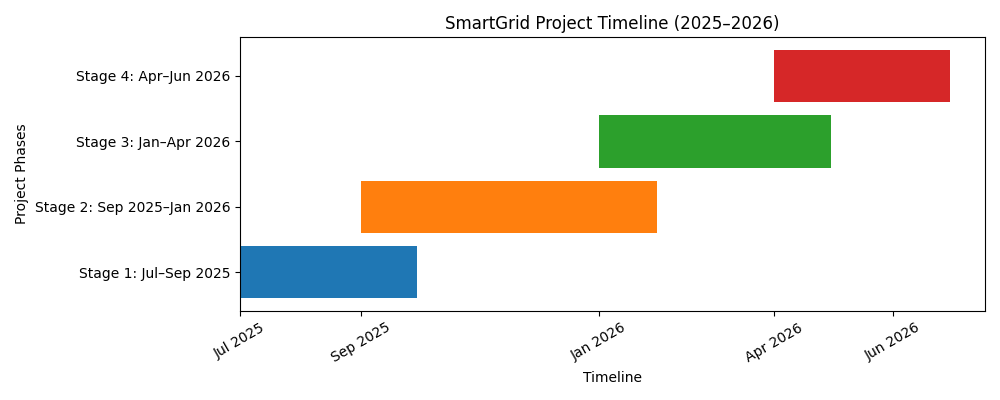
\includegraphics[width=0.9\textwidth]{chart.png}}
\caption{Project timeline }
\label{fig:Gantt Chart}
\end{figure}


\noindent
The project timeline is structured into four overlapping stages spanning July 2025 to June 2026, reflecting the iterative and incremental development approach adopted in this work. 

Stage 1 (July--September 2025) focuses on problem formulation, dataset preparation, and baseline experimentation. Stage 2 (September 2025--January 2026) involves feature engineering and prototype development, including the initial implementation of the anomaly detection framework. Stage 3 (January--April 2026) covers model refinement, system integration, and full evaluation across different configurations. Finally, Stage 4 (April--June 2026) is dedicated to documentation, system packaging, and preparation for final presentation and defense.

The overlap between stages shows parallel progress, where findings from later phases fed back into earlier design decisions and led to ongoing changes throughout the project.

\printbibliography
\end{document}
